\documentclass[11pt]{report}
\usepackage[a4paper, left=2cm, right=2cm, top=2.5cm, bottom=2.5cm]{geometry}
\usepackage{theme}
\usepackage{shortcuts}

\usepackage{graphicx}
\usepackage{amsmath,amssymb}
\usepackage{booktabs}
\usepackage{multirow}
\usepackage{float}
\usepackage{tikz}
\usetikzlibrary{positioning}

\usepackage{algorithm}
\usepackage{algorithmicx}
\usepackage{algpseudocode}

\usepackage{titlesec}
\titlespacing*{\paragraph}
  {0pt}     % left indent
  {5pt}     % space BEFORE
  {5pt}     % space AFTER

\usepackage[style=numeric]{biblatex}
\addbibresource{bibliography.bib}

% Document parameters
% Document title
\title{
      \LARGE{CentraleSupélec - Mathematics and Data Science}
      \\ \Large{Research Project Report - 2025/2026}
      \\ \large{Probabilistic Detection of Market Manipulation}
      }

\author{
      Adonis JAMAL \quad Jean-Vincent MARTINI
      \\ Supervisor: Damien CHALLET
}

\date{April 2026}

% ==============================================================================
% ================================== DOCUMENT ==================================  
% ==============================================================================
\begin{document}


% ==============================================================================
% SECTION: TITLE PAGE 
% ==============================================================================
\begin{titlepage}
\centering

{\Large CentraleSup\'elec\par}
\vspace{0.2cm}
{\large Mathematics and Data Science\par}

\vspace{1.2cm}
{\Large\bfseries Research Project Report\par}
\vspace{0.2cm}
{\large Academic Year 2025-2026\par}

\vspace{1.2cm}
{\huge\bfseries Probabilistic Detection of Market Manipulation\par}

\vspace{2.0cm}

{\large
Adonis JAMAL \quad Jean-Vincent MARTINI\par
}
\vspace{0.5cm}
{\large Supervisor: Damien CHALLET\par}
\vspace{0.2cm}
{\large Academic Tutor: Lionel GABET\par}

\vfill

{\large April 2026\par}
\vspace{1.0cm}

\begin{minipage}[c]{0.42\textwidth}
\centering

\includegraphics[height=1.8cm]{img/logoMICS.png}
\end{minipage}
\hfill
\begin{minipage}[c]{0.42\textwidth}
\centering

\includegraphics[height=1.8cm]{img/logo_cs.png}
\end{minipage}

\end{titlepage}


% ==============================================================================
% ABSTRACT
% ==============================================================================
\chapter*{Abstract}
Detecting market manipulation such as spoofing, layering, and quote stuffing in limit order books presents a significant challenge due to the lack of labelled data. This research introduces a multi-model unsupervised detection pipeline evaluated on equity limit order book data. The methodology integrates three complementary models: a Transformer bottleneck autoencoder coupled with a One-Class SVM, a Probabilistic Neural Network, and a Probabilistic Robust Autoencoder. These models process 89 engineered features, including Hawkes-inspired and microstructural indicators. To generate actionable alerts from continuous anomaly scores, the system deploys adaptive Extreme Value Theory thresholds alongside interpretability methods. The results detail anomaly rates across various time periods, establish cross-year model stability, map the cluster structure of flagged events, and quantify economic spoofing gain estimates. This work demonstrates a multi-model unsupervised pipeline, successfully combining probabilistic density estimation, robust autoencoders, and economic gain quantification on a single limit order book dataset. The codebase for this project is available at \url{https://github.com/adonis107/MDS-PDMM}.


% ==============================================================================
% ACKNOWLEDGEMENTS
% ==============================================================================
\chapter*{Acknowledgements}
We would like to express our sincere gratitude to our supervisor, Damien Challet, for his continuous guidance, keen interest, the attention he dedicated to our project, and the weekly meetings that kept this project on track. We are also grateful to him for providing access to the necessary data for our research.

We extend our thanks to our academic tutor, Lionel Gabet, for his valuable feedback, academic guidance, and for closely following the project's progression throughout the year. His engagement and constructive critiques during our presentations were highly appreciated.

Finally, we acknowledge the Ruche HPC cluster at Université Paris-Saclay for providing the GPU compute resources essential for training our models.


% ==============================================================================
% TABLE OF CONTENTS
% ==============================================================================
\newpage
\tableofcontents


% ==============================================================================
% CHAPTER 1: INTRODUCTION
% ==============================================================================
\chapter{Introduction}\label{chap:intro}

\section{Context and Motivation}\label{sec:intro:context}

Modern securities exchanges organise trading through electronic limit order books. A limit order book (LOB) records all outstanding buy and sell orders at each price level, providing a real-time, public summary of supply and demand. The instantaneous state of the book, defined by the distribution of volume across price levels on both sides, and the recent flow of incoming orders jointly determine short-term price dynamics. Tao et al.~\cite{tao_2020} model this dependence through a multi-level volume imbalance that aggregates supply and demand across several price levels, showing on TMX data that imbalance shifts are directly linked to the probability distribution of subsequent price moves. Fabre and Challet~\cite{fabre_2025} extend this line of work by introducing Hawkes-inspired order flow features that capture both the size and the distance of placement of new limit orders, demonstrating on cryptocurrency data that these features predict the conditional distribution of mid-price movements.

Market manipulation exploits this dependence. By artificially altering either the instantaneous book state or the order flow, a manipulator can induce a predictable price response and profit from it. Spoofing, the primary focus of this project, consists of placing large visible limit orders with no intention of execution. These orders shift the perceived supply-demand balance, move the mid-price in the desired direction, and are cancelled once the manipulator's genuine order on the opposite side has been filled. Layering extends spoofing by stacking multiple non-bona-fide orders across several price levels, amplifying the perceived depth on one side of the book~\cite{fabre_2025}. Both strategies distort the volume imbalance: Tao et al.~\cite{tao_2020} show that the optimal spoofing action shifts the multi-level imbalance away from its equilibrium value, and that comparing the observed imbalance before a market order to its long-run distribution provides a basis for detection.

The regulatory treatment of these strategies differs sharply between asset classes. In regulated equity and derivatives markets, spoofing and layering are explicitly prohibited under the European Market Abuse Regulation (EU MAR) and the US Dodd-Frank Act. In cryptocurrency markets, the absence of equivalent regulation opens the door to manipulative behaviour on a larger scale~\cite{fabre_2025}. Fabre and Challet, working on Level-3 crypto order book data, find that 31\% of large orders on the BTC-USD and ETH-USD pairs could profitably spoof the market over a four-day period. This asymmetry suggests that crypto order book data should contain a substantially higher base rate of manipulative patterns than equity data.
The present work focuses on the more challenging equity setting, where manipulation is rarer and must be detected without labels.

\paragraph{Why unsupervised, score-based detection.}\label{sec:intro:problem}
A binary classifier that labels each event as ``manipulative'' or ``not'' is poorly suited to this detection problem for three reasons. First, no ground-truth labels exist: in equity markets, confirmed manipulation cases are rare and not publicly annotated at the order level. Second, manipulation is not a discrete category but a spectrum of intent, from aggressive but legitimate liquidity provision to unambiguous spoofing. Third, a probabilistic score is more actionable than a binary flag: it allows a surveillance system to rank events by severity and calibrate alert thresholds to a desired false discovery rate. Fabre and Challet~\cite{fabre_2025} address these requirements with a probabilistic neural network that outputs a full predictive distribution over future price moves, from which both an anomaly score (the negative log-likelihood) and an economic spoofing gain estimate (formalised in Section~\ref{sec:methodology:spoofing}) can be derived.


\section{Research Questions}\label{sec:intro:questions}

This project investigates the following questions:

\begin{enumerate}
    \item Can unsupervised probabilistic models trained on order book features detect anomalous order flow in the absence of ground-truth labels?
    \item Which order book features carry the most information about anomalous events, and do different detection models agree on the same discriminative features?
    \item How should anomaly thresholds be calibrated in a non-stationary, streaming setting when no labelled data are available?
    \item Can the economic profitability of a spoofing strategy be estimated directly from model predictions, providing an interpretable measure of manipulation opportunity?
    \item Do detection patterns remain stable across different time periods, when models trained on one year are applied to data from other years?
\end{enumerate}

These questions are addressed on the TOTF.PA (TotalEnergies, Euronext Paris) limit order book dataset, covering trading days from 2010, 2015, and 2017.


\section{Contributions}\label{sec:intro:contributions}

The main contributions of this report are:

\begin{enumerate}
    \item A modular detection pipeline that combines three complementary unsupervised models on the same equity LOB dataset (TOTF.PA, Euronext Paris): a Transformer bottleneck autoencoder inspired by Poutr\'e et al.~\cite{poutre_2024}, coupled with a Nystr\"om-approximated One-Class SVM in latent space; a Probabilistic Neural Network (PNN) that predicts skew-normal price move distributions following the framework of Fabre and Challet~\cite{fabre_2025}; and a Probabilistic Robust Autoencoder (PRAE) with learnable per-sample gates~\cite{lindenbaum2022prae}. Each model produces a scalar anomaly score per time step; their agreement identifies the highest-confidence anomalies.

    \item A feature engineering library of 89 features synthesising contributions from multiple sources: Hawkes-inspired memory features with spatial and temporal decay~\cite{fabre_2025}, weighted multi-level volume imbalance~\cite{tao_2020}, event flow and cancellation rapidity~\cite{poutre_2024}, multi-level order flow imbalance, and standard microstructural indicators (spread, volatility, elasticity).
      This represents an input space roughly seven times larger than that of Poutr\'e et~al.~\cite{poutre_2024}, who use approximately 13~Level-1 features.

    \item Application of the spoofing gain framework of Fabre and Challet~\cite{fabre_2025} to equity LOB data.  The PNN-predicted skew-normal parameters feed an expected cost model that quantifies the profitability of a hypothetical spoofing strategy at each time step, producing an interpretable economic measure of manipulation opportunity.

    \item A systematic comparison of four threshold methods for converting continuous anomaly scores into binary alerts without labels: Peak Over Threshold (POT), Streaming POT (SPOT), Drift-aware Streaming POT (DSPOT)~\cite{siffer:hal-01640325}, and a rolling Benjamini-Hochberg False Discovery Rate controller (RFDR).

    \item Interpretability analysis via Integrated Gradients~\cite{sundararajan2017axiomaticattributiondeepnetworks} for the PNN and PRAE, and Grouped Occlusion for the Transformer+OC-SVM, identifying which feature families and which sides of the order book drive each model's anomaly scores.

    \item Post-hoc characterisation of detected anomalies through HDBSCAN clustering of the three anomaly scores and microstructural jump analysis (bipower variation, variance ratio, CUSUM), providing an unsupervised taxonomy of anomaly types.

    \item Cross-year robustness evaluation: models trained on 2015 data are tested on 2010, 2015, and 2017 data, and models trained on 2017 data are tested on the same periods, assessing whether the pipeline detects consistent patterns across different market regimes.
\end{enumerate}


\section{Report Outline}\label{sec:intro:outline}

Chapter~\ref{chap:background} reviews the literature on limit order book microstructure, market manipulation, and the detection methods that this project builds on.
Chapter~\ref{chap:methodology} formalises the feature engineering pipeline, the three detection models with their loss functions, the threshold methods, the spoofing gain framework, and the interpretability and post-hoc analysis tools.
Chapter~\ref{chap:data} describes the TOTF.PA dataset, the preprocessing steps, the sequential training protocol, and the experimental setup.
Chapter~\ref{chap:results} presents the experimental findings: model diagnostics, anomaly detection rates, threshold comparisons, sensitivity analysis, anomaly clustering, jump analysis, and cross-year robustness.
Chapter~\ref{chap:discussion} discusses the limitations of the approach, compares the three detection models, and interprets the detected anomalies in light of known manipulation signatures.
Chapter~\ref{chap:conclusion} summarises the contributions and outlines directions for future work.


% ==============================================================================
% CHAPTER 2: BACKGROUND AND RELATED WORK
% ==============================================================================
\chapter{Background and Related Work}\label{chap:background}

This chapter provides the conceptual vocabulary and critical perspective needed to evaluate the methodological choices presented in Chapter~\ref{chap:methodology}. Each section introduces a class of approaches, explains what it is good at, where it struggles, and what assumptions it makes. Formal definitions, model architectures, and training procedures are deferred to Chapter~\ref{chap:methodology}.

\section{Limit Order Books and Market Microstructure}\label{sec:background:lob}

A limit order book records all outstanding buy and sell orders for a security, organised by price and submission time. At time~$t$, the book state consists of $L$ price levels on each side. The bid (buy) side lists prices $p^b_1 > p^b_2 > \cdots > p^b_L$ with corresponding volumes $v^b_1, v^b_2, \ldots, v^b_L$. The ask (sell) side lists prices $p^a_1 < p^a_2 < \cdots < p^a_L$ with volumes $v^a_1, v^a_2, \ldots, v^a_L$. The best bid is~$p^b_1$, the best ask is~$p^a_1$, the mid-price is $p_{\text{mid}} = (p^a_1 + p^b_1)/2$, and the spread is $s = p^a_1 - p^b_1$.

Three event types modify the book state. A \emph{limit order} adds volume at a specified price level, increasing liquidity. A \emph{cancellation} removes a previously placed limit order, reducing liquidity at that level. A \emph{market order} (equivalently, a trade) consumes volume at the best price on the opposite side, removing liquidity and potentially shifting the best price.

The instantaneous distribution of volume across price levels and the temporal sequence of these events jointly determine short-term price dynamics. Volume imbalance, the normalised excess of bid over ask volume at a given level, is a widely used summary statistic of the book state. Tao et~al.~\cite{tao_2020} extend the single-level imbalance to a weighted multi-level measure that aggregates supply and demand across several price levels, and show on TMX (Toronto Stock Exchange) data that this quantity is directly linked to the probability distribution of subsequent price moves. Fabre and Challet~\cite{fabre_2025} complement imbalance with Hawkes-inspired features that capture both the size and the spatial placement depth of new limit orders, demonstrating on cryptocurrency data that these features predict the conditional distribution of mid-price movements.

\section{Market Manipulation Strategies}\label{sec:background:manipulation}

Spoofing consists of submitting large, visible limit orders with no intention of execution to create a false impression of supply or demand. The lifecycle of a spoofing event follows a characteristic sequence:
(1)~the manipulator places one or more large limit orders on one side of the book, shifting the perceived imbalance;
(2)~the mid-price moves in the direction favoured by the manipulator;
(3)~the manipulator executes a genuine order on the opposite side at the improved price;
(4)~the non-bona-fide orders are cancelled.
Layering extends spoofing by stacking multiple orders across several price levels on the same side, amplifying the perceived depth~\cite{fabre_2025}. Quote stuffing is a related strategy in which a large number of orders are rapidly submitted and cancelled to flood the matching engine with messages, degrading other participants' ability to process market data and exploiting the resulting informational advantage. Unlike spoofing, quote stuffing operates primarily through message-rate pressure rather than through direct manipulation of the perceived volume imbalance.

Both spoofing and layering are prohibited under the European Market Abuse Regulation (EU MAR, Article~12) and the US Dodd-Frank Act (Section~747). Detection is challenging because the same order flow patterns can arise from legitimate trading strategies, such as aggressive liquidity provision or inventory management. Tao et~al.~\cite{tao_2020} formalise the detection problem by modelling the imbalance shift caused by a spoof order and comparing the observed pre-trade imbalance distribution to its long-run counterpart via the Wasserstein distance. Fabre and Challet~\cite{fabre_2025} take an economic approach: rather than asking whether an order flow pattern looks abnormal, they ask whether a rational spoofer could profit from the current book state, defining the spoofing gain as the difference in expected execution cost between a scenario where the spoof order is present and one where it is absent.

The arguments for unsupervised, score-based detection over binary classification are detailed in Section~\ref{sec:intro:problem} and are not repeated here.

\section{Anomaly Detection in Financial Data}\label{sec:background:anomaly}

In the absence of ground-truth labels for manipulation, detection must proceed unsupervised. A central difficulty shared by all unsupervised approaches is the \emph{contamination problem}: training data collected from a real market inevitably contains some anomalous events, and their presence can degrade the learned model of normality. This section surveys three families of approaches and discusses their relative strengths and weaknesses for the LOB anomaly detection problem.

\subsection{Reconstruction-Based Approaches}\label{subsec:background:reconstruction}

Autoencoders learn a compressed representation of the training data and reconstruct each input from that representation. When the training set is predominantly normal, the model learns to reconstruct normal patterns well; anomalous inputs produce high reconstruction error because they deviate from the learned structure. This family has several merits: it requires no labels, captures complex multivariate dependencies, and generalises across instruments and time periods without task-specific supervision.

For order book sequences, the choice of encoder architecture matters. Convolutional and recurrent architectures capture local patterns effectively but struggle with long-range dependencies between distant price levels or between events separated by many time steps. The Transformer architecture addresses this limitation through self-attention, which allows each position in the sequence to attend directly to every other position. Multi-head attention enables the model to simultaneously capture different aspects of the book state, such as volume dynamics at the top of the book, spread behaviour, and order arrival patterns deeper in the queue. Poutr\'e et~al.~\cite{poutre_2024} demonstrate on NASDAQ LOBSTER data that a Transformer autoencoder combined with a one-class classifier in the latent space outperforms the reconstruction error alone for detecting synthetically injected manipulation patterns (quote stuffing, layering, and pump-and-dump). Notably, their feature set is built from Level-1 (best bid/ask) data only, yielding approximately 13~features; the present work extends this approach to Level-2 (ten price levels per side) data with roughly 80~features, which introduces both richer information and a substantially higher-dimensional input space.

A limitation of deterministic autoencoders is that the reconstruction error is a noisy proxy for anomaly severity: it does not distinguish between inputs that are merely unusual and inputs that fall outside the training distribution entirely. A probabilistic formulation, in which the autoencoder outputs a distribution over reconstructions rather than a point estimate, addresses this limitation by providing an uncertainty signal. Lindenbaum et~al.~\cite{lindenbaum2022prae} go further: rather than modifying the reconstruction itself, they introduce learnable per-sample gates that allow the training procedure to downweight suspected anomalies, so that the autoencoder focuses on reconstructing clean data even when the training set is contaminated. This makes the model robust to the contamination problem without requiring an explicit data-cleaning step. The degree of contamination in the specific TOTF.PA dataset is unknown; the PRAE's robustness is therefore a precautionary measure rather than a response to a measured contamination rate.

\subsection{Probabilistic Scoring via Synthetic Manipulation}\label{subsec:background:scoring}

An alternative to asking ``does this look abnormal?''\ is to ask ``how much could a rational spoofer gain from this book state?'' Fabre and Challet~\cite{fabre_2025} pursue this reframing by training a probabilistic neural network that predicts the full conditional distribution of the next mid-price move. The predicted distribution serves two purposes: its negative log-likelihood provides a general anomaly score (events where the realised price move is unlikely under the model receive high scores), and its parameters feed an expected cost model that quantifies the profitability of a hypothetical spoofing strategy at each time step.

The merits of this approach are substantial. The spoofing gain score has a direct economic interpretation, which makes it more actionable for a market surveillance system than a generic reconstruction error. Training on the predictive task sidesteps the need for labelled manipulation data: the model learns normal price dynamics, and deviations from that model are flagged regardless of their cause. The probabilistic output naturally quantifies uncertainty over the predicted price move, which matters for heavy-tailed financial data where point predictions are unreliable.

The limitations are equally clear. The spoofing gain depends on a model of the spoofer's strategy (order size, placement distance, fee structure), so it may miss manipulation patterns that deviate from that model. The approach was developed and evaluated on cryptocurrency LOB data (BTC-USD and ETH-USD on Coinbase)~\cite{fabre_2025}, where the absence of anti-manipulation regulation results in a higher base rate of manipulative behaviour; its effectiveness on regulated equity markets, where manipulation is rarer and subtler, has not been established in the literature.

\subsection{One-Class and Density-Based Approaches}\label{subsec:background:oneclass}

One-class classification methods learn a tight boundary around the training data in a transformed feature space and flag anything outside that boundary as anomalous. The One-Class SVM (OC-SVM) is the most widely used instance: it finds a hyperplane in a kernel-induced feature space that separates the data from the origin with maximum margin, controlled by a parameter $\nu$ that bounds the fraction of training points allowed outside the boundary.

The strengths of the OC-SVM are computational efficiency and theoretical simplicity. It does not require specifying what an anomaly looks like, only what normal data looks like, and the kernel trick allows it to capture non-linear structure in the input space. However, it does not scale well to high-dimensional feature spaces without careful kernel design: in the 89-dimensional feature space typical of LOB anomaly detection, the RBF kernel becomes poorly calibrated and the decision boundary may either collapse or become too loose. Low-rank kernel approximations (such as the Nystr\"om method) partially address this issue by projecting the kernel evaluation into a tractable subspace, enabling GPU-accelerated training. A further limitation is that the OC-SVM does not produce a calibrated probability; its decision function is a signed distance, not a likelihood, which complicates downstream interpretation and threshold calibration.

For the LOB problem, the OC-SVM is most effective when applied not to raw features but to a learned latent representation. Poutr\'e et~al.~\cite{poutre_2024} demonstrate this by fitting an OC-SVM in the bottleneck space of a Transformer autoencoder, where the reduced dimensionality and the learned structure of the representation make the kernel boundary more discriminative. This two-stage approach combines the representation power of reconstruction-based methods with the boundary-learning capacity of one-class classification.

\section{Thresholding Methods for Anomaly Detection}\label{sec:background:thresholding}

Any continuous anomaly score requires a threshold to produce a detection decision. The naive approach, a fixed percentile of the score distribution, assumes that the distribution is stationary and well-behaved. In financial data, score distributions are heavy-tailed and non-stationary: a fixed percentile will produce too many false positives during volatile periods and miss anomalies during quiet periods. Setting thresholds without labels is therefore a problem in its own right.

\paragraph{Extreme Value Theory (EVT).}
EVT models the tail of the score distribution rather than the bulk, fitting a Generalised Pareto Distribution to the exceedances above a high initial threshold. This is well-suited to heavy-tailed data because the statistical guarantee applies specifically to extreme quantiles, where fixed-percentile methods are least reliable. Siffer et~al.~\cite{siffer:hal-01640325} extend the batch EVT estimator to streaming settings with two algorithms: SPOT, which updates the tail model as new peaks arrive, and DSPOT, which adds a drift correction that tracks shifts in the baseline score level over time. The main assumption is that the tail of the score distribution is well-approximated by the GPD, which must be verified empirically for each model output.

\paragraph{False Discovery Rate (FDR) Control.}
FDR-based procedures, such as the Benjamini-Hochberg method, control the expected proportion of false positives among all flagged events. This is appropriate when anomalies are rare and the cost of false positives is high, because it bounds the discovery error rate rather than the absolute false positive count. The requirement is a set of p-values or a reference null distribution for the anomaly score, which must be estimated from the data when no parametric form is available.

\paragraph{Rolling FDR (RFDR).}
RFDR adapts the Benjamini-Hochberg procedure to a streaming setting by maintaining a sliding window of recent anomaly scores. Within each window, scores are log-transformed, converted to robust z-scores using the median absolute deviation, and mapped to p-values under a Gaussian assumption; the BH procedure then determines a dynamic threshold that controls the false discovery rate at level~$\alpha$. Because the null distribution is re-estimated at every step from the local window, RFDR tracks non-stationarity in the score distribution without requiring an explicit drift model.

\paragraph{Implicit and Post-Hoc Model Thresholds.}
Some detection methods appear to produce a threshold as a byproduct of training. The OC-SVM decision boundary, for instance, defines a binary classification in the feature space: points with negative decision function values are labelled as outliers. However, in practice this binary output is often discarded in favour of a continuous dissimilarity score, and a separate threshold is selected post-hoc on labelled evaluation data. Poutr\'e et~al.~\cite{poutre_2024} follow this approach, choosing the threshold that maximises the $F_4$-score on a test set containing synthetic manipulations. This converts an ostensibly unsupervised method into one that depends on labelled data for threshold calibration.

\section{Feature Attribution Methods}\label{sec:background:attribution}

A detection score alone is not actionable for a market surveillance analyst: the analyst needs to know which features of the order book drove the score and whether those features align with known manipulation signatures. Attribution for sequential financial data is harder than for static inputs because features at different time steps and price levels are structurally correlated, and because the underlying distribution shifts over the trading day.

Two broad families of attribution methods are relevant. Gradient-based methods, such as Integrated Gradients~\cite{sundararajan2017axiomaticattributiondeepnetworks}, accumulate the model's gradient along a path from a baseline input to the actual input, producing per-feature importance scores that are theoretically principled (they satisfy completeness and sensitivity axioms) and computationally tractable. Their limitation is that they require a differentiable end-to-end model, which excludes pipelines where a non-differentiable component (such as an OC-SVM) sits between the learned representation and the final score.

For non-differentiable pipelines, ablation-based methods provide an alternative. Grouped occlusion replaces semantically related groups of features (all bid-side features, all Hawkes features, all features at a given price level) with a baseline value and measures the resulting change in the anomaly score. This approach is model-agnostic and handles the structured correlation among LOB features by operating at the group level rather than the individual feature level. The trade-off is lower resolution: it identifies which feature families matter, not which individual features within a family are most important.


% ==============================================================================
% CHAPTER 3: METHODOLOGY
% ==============================================================================
\chapter{Methodology}\label{chap:methodology}

\begin{figure}[H]
\centering
\resizebox{\textwidth}{!}{%
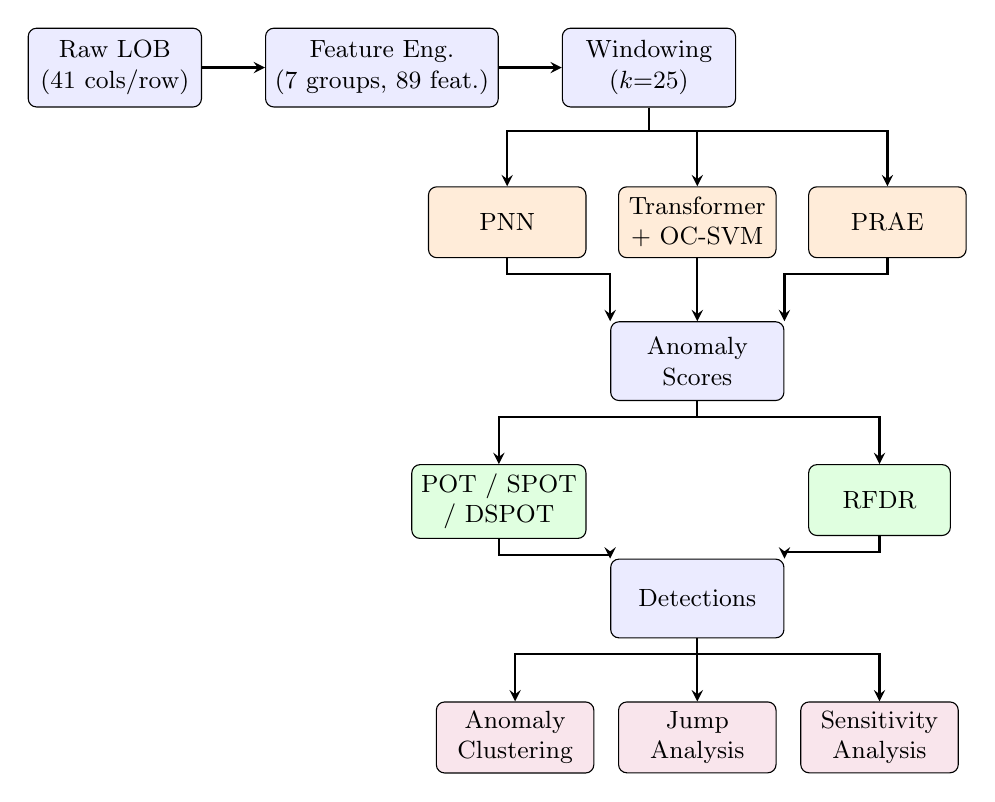
\begin{tikzpicture}[
  node distance=0.6cm and 0.8cm,
  stage/.style={rectangle, draw, rounded corners=3pt, minimum height=1cm, minimum width=2.2cm,
                align=center, font=\small, fill=blue!8},
  model/.style={rectangle, draw, rounded corners=3pt, minimum height=0.9cm, minimum width=2cm,
                align=center, font=\small, fill=orange!15},
  threshold/.style={rectangle, draw, rounded corners=3pt, minimum height=0.9cm, minimum width=1.8cm,
                    align=center, font=\small, fill=green!12},
  posthoc/.style={rectangle, draw, rounded corners=3pt, minimum height=0.9cm, minimum width=2cm,
                  align=center, font=\small, fill=purple!10},
  arr/.style={->, thick, >=stealth},
]
  % Row 1: Data pipeline
  \node[stage] (raw) {Raw LOB\\(41 cols/row)};
  \node[stage, right=of raw] (feat) {Feature Eng.\\(7 groups, $89$ feat.)};
  \node[stage, right=of feat] (win) {Windowing\\($k{=}25$)};

  % Row 2: Models
  \node[model, below right=1.0cm and -1.5cm of win] (tfocsvm) {Transformer\\+ OC-SVM};
  \node[model, left=0.4cm of tfocsvm] (pnn) {PNN};
  \node[model, right=0.4cm of tfocsvm] (prae) {PRAE};

  % Row 3: Scores
  \node[stage, below=0.8cm of tfocsvm] (scores) {Anomaly\\Scores};

  % Row 4: Thresholding
  \node[threshold, below left=0.8cm and 0.3cm of scores] (evt) {POT / SPOT\\/ DSPOT};
  \node[threshold, below right=0.8cm and 0.3cm of scores] (rfdr) {RFDR};

  % Row 5: Detections
  \node[stage, below=0.8cm of scores, yshift=-1.2cm] (det) {Detections};

  % Row 6: Post-hoc
  \node[posthoc, below left=0.8cm and 0.2cm of det] (clust) {Anomaly\\Clustering};
  \node[posthoc, below=0.8cm of det] (jump) {Jump\\Analysis};
  \node[posthoc, below right=0.8cm and 0.2cm of det] (ig) {Sensitivity\\Analysis};

  % Arrows
  \draw[arr] (raw) -- (feat);
  \draw[arr] (feat) -- (win);
  \draw[arr] (win.south) -- ++(0,-0.3) -| (pnn.north);
  \draw[arr] (win.south) -- ++(0,-0.3) -| (tfocsvm.north);
  \draw[arr] (win.south) -- ++(0,-0.3) -| (prae.north);
  \draw[arr] (pnn.south) -- ++(0,-0.2) -| (scores.north west);
  \draw[arr] (tfocsvm.south) -- (scores.north);
  \draw[arr] (prae.south) -- ++(0,-0.2) -| (scores.north east);
  \draw[arr] (scores.south) -- ++(0,-0.2) -| (evt.north);
  \draw[arr] (scores.south) -- ++(0,-0.2) -| (rfdr.north);
  \draw[arr] (evt.south) -- ++(0,-0.2) -| (det.north west);
  \draw[arr] (rfdr.south) -- ++(0,-0.2) -| (det.north east);
  \draw[arr] (det.south) -- ++(0,-0.2) -| (clust.north);
  \draw[arr] (det.south) -- (jump.north);
  \draw[arr] (det.south) -- ++(0,-0.2) -| (ig.north);
\end{tikzpicture}%
}
\caption{End-to-end detection pipeline. Raw LOB snapshots are transformed into ${\sim}85$ features, windowed into sequences of length $k{=}25$, and scored by three complementary models. Threshold methods produce binary detections, which are analysed post hoc via clustering, jump tests, and integrated-gradient attribution.}
\label{fig:pipeline}
\end{figure}

\section{Feature Engineering}\label{sec:methodology:features}

The raw limit order book data for TOTF.PA (TotalEnergies, Euronext Paris) records the state of the book at each update event during continuous trading hours (09:00-17:30 CET). Each row contains an Excel serial timestamp $t$ (column \texttt{xltime}, where the fractional part encodes the time of day) and the price and volume at $L = 10$ levels on each side: $p^b_1, V^b_1, \ldots, p^b_{10}, V^b_{10}$ for the bid and $p^a_1, V^a_1, \ldots, p^a_{10}, V^a_{10}$ for the ask, giving 41 columns per row. The data is event-driven: a new row is recorded whenever a limit order, cancellation, or trade modifies the visible book state, so the inter-event spacing is irregular.

Feeding the 40 raw price-volume columns directly to a model is wasteful and fragile. Prices at adjacent levels are highly correlated, volumes are non-stationary, and the absolute price level carries no information about short-term dynamics. Engineered features reduce the input dimensionality to $d_{\text{in}} = 89$ informative quantities that are more stationary, more interpretable, and encode the domain knowledge needed to distinguish normal from anomalous order flow.

The features are organised into seven groups: (1)~order book imbalance, capturing supply-demand asymmetry across depth levels; (2)~price dynamics and microstructure, summarising price movements and their relationship to volume; (3)~liquidity and elasticity, measuring the cost and shape of the book; (4)~volatility proxies; (5)~event flow and rapidity, characterising the intensity and type of order arrivals; (6)~Hawkes-inspired memory features, capturing self-exciting patterns in order flow with spatial and temporal decay; and (7)~order flow imbalance, measuring signed directional pressure from volume changes conditioned on price movements. Preprocessing and scaling are described in Section~\ref{subsec:features:preprocessing}.


\subsection{Order Book Imbalance}\label{subsec:features:imbalance}

Imbalance features quantify the asymmetry between supply and demand at various depths of the book. Spoofing and layering distort this asymmetry by injecting volume on one side; imbalance measures are therefore among the most direct indicators of manipulative intent.

The Level-1 imbalance compares bid and ask volume at the best quotes:
\begin{equation}
  \label{eq:l1_imbalance}
  I^{(1)}_t = \frac{V^b_{1,t} - V^a_{1,t}}{V^b_{1,t} + V^a_{1,t}}.
\end{equation}
Values near $+1$ indicate strong buy-side pressure; values near $-1$ indicate sell-side pressure.

The Level-5 imbalance aggregates volume across the top five levels on each side:
\begin{equation}
  \label{eq:l5_imbalance}
  I^{(5)}_t = \frac{\sum_{i=1}^{5} V^b_{i,t} - \sum_{i=1}^{5} V^a_{i,t}}{\sum_{i=1}^{5} V^b_{i,t} + \sum_{i=1}^{5} V^a_{i,t}}.
\end{equation}
A divergence between $I^{(1)}_t$ and $I^{(5)}_t$ suggests that volume is concentrated away from the best quotes, a pattern consistent with layering.

To weight deeper levels more flexibly, we follow Tao et~al.~\cite{tao_2020} and define a weighted multi-level imbalance over $L = 5$ levels with weight vector $\mathbf{w} = (w_1, \ldots, w_5)$:
\begin{equation}
  \label{eq:weighted_imbalance}
  I^{(\mathbf{w})}_t = \frac{\sum_{i=1}^{5} w_i \, V^b_{i,t}}{\sum_{i=1}^{5} w_i \, V^b_{i,t} + \sum_{i=1}^{5} w_i \, V^a_{i,t}}.
\end{equation}
This quantity lies in $[0, 1]$; values above $0.5$ indicate net bid-side weight. Three weight configurations are used: \emph{decreasing-weighted} $\mathbf{w} = (0.1, 0.1, 0.2, 0.2, 0.4)$, which emphasises deeper levels where spoof orders are less likely to be executed; \emph{increasing-weighted} $\mathbf{w} = (0.4, 0.2, 0.2, 0.1, 0.1)$, which emphasises the best quotes; and \emph{constant-weighted} $\mathbf{w} = (0.2, 0.2, 0.2, 0.2, 0.2)$, which weights all five levels equally. Unlike the Level-1 volume imbalance used by Poutr\'e et~al.~\cite{poutre_2024}, this weighted formulation aggregates information across five price levels, so $I^{(\mathbf{w})}_t$ reflects the depth structure of the book rather than only the best quotes.


\subsection{Price Dynamics and Microstructure}\label{subsec:features:price}

This group captures the immediate state of the price process and its first- and second-order dynamics.

The mid-price and bid-ask spread are:
\begin{equation}
  \label{eq:midprice}
  p_{\text{mid},t} = \frac{p^a_{1,t} + p^b_{1,t}}{2}, \qquad
  s_t = p^a_{1,t} - p^b_{1,t}.
\end{equation}

The micro-price deviation measures how far the L1-imbalance-adjusted fair value lies from the mid-price:
\begin{equation}
  \label{eq:microprice_deviation}
  \delta_t^{\text{micro}} = I^{(1)}_t \cdot \frac{s_t}{2}.
\end{equation}
A large deviation suggests that the balance of volume at the best quotes is pulling the fair value away from the geometric centre of the spread.

The volume depth ratio measures the concentration of volume away from the best quote on each side $s \in \{b, a\}$:
\begin{equation}
  \label{eq:depth_ratio}
  D^s_t = \frac{\sum_{i=2}^{5} V^s_{i,t}}{V^s_{1,t}}.
\end{equation}
High values indicate that most liquidity sits behind the best quote, a signature of layering where large volumes are placed at deeper levels.

Log returns, velocity, and acceleration of the mid-price are:
\begin{equation}
  \label{eq:log_return}
  r_t = \ln\!\left(\frac{p_{\text{mid},t}}{p_{\text{mid},t-1}}\right), \quad
  v_t = p_{\text{mid},t} - p_{\text{mid},t-1}, \quad
  a_t = v_t - v_{t-1}.
\end{equation}

The net order flow at Level~1 isolates volume changes that occur at a fixed price, filtering out changes caused by price-level shifts:
\begin{equation}
  \label{eq:net_flow}
  F^s_t = \Delta V^s_{1,t} \cdot \mathbf{1}\!\left[p^s_{1,t} = p^s_{1,t-1}\right], \qquad s \in \{b, a\},
\end{equation}
where $\Delta V^s_{1,t} = V^s_{1,t} - V^s_{1,t-1}$.
A large positive $F^b_t$ followed by a rapid cancellation is a textbook spoofing pattern.

Volume deltas $\Delta V^b_{1,t}$ and $\Delta V^a_{1,t}$ at the best quotes are also retained as raw features, along with the rolling standard deviation of the mid-price over a window of $W = 50$ events.


\subsection{Liquidity and Elasticity}\label{subsec:features:liquidity}

These features describe how much it costs to execute a given order size and how steeply the book's price schedule rises with volume.

The sweep-to-fill cost is the volume-weighted average price paid to execute a target order of size $Q = 1{,}000$ units by walking through $L = 10$ levels. The value $Q = 1{,}000$ was chosen empirically to represent a moderately sized institutional order for TOTF.PA; no reference paper prescribes a specific target size, and a sensitivity analysis over $Q$ is deferred to Chapter~\ref{chap:results}. Denoting by $C^s_t(Q)$ the resulting average execution price on side $s$, the reported features are the excess costs relative to the mid-price:
\begin{equation}
  \label{eq:sweep_cost}
  \text{SC}^a_t = C^a_t(Q) - p_{\text{mid},t}, \qquad
  \text{SC}^b_t = p_{\text{mid},t} - C^b_t(Q).
\end{equation}
Both quantities are non-negative under normal conditions. Large values indicate thin liquidity: a spoofing episode that removes genuine orders from the book can cause a spike in sweep cost.

The book slope (elasticity) measures the sensitivity of price to cumulative volume. For each side $s$, a linear regression of price on log cumulative volume across the first $D = 5$ levels gives the following relationship (Tao et~al.~\cite{tao_2020} calibrate a comparable depth parameter to values between 3 and 5 depending on the stock; Fabre and Challet~\cite{fabre_2025} use $K = 5$ as a representative depth): The depth $D = 5$ is consistent with the range used by Tao et~al.~\cite{tao_2020} (who calibrate 3 to 5 depending on the stock) and Fabre and Challet~\cite{fabre_2025} (who use $K = 5$); an ablation over $D$ is reported in Chapter~\ref{chap:results}.
\begin{equation}
  \label{eq:book_slope}
  p^s_{i,t} \approx \alpha^s_t + \beta^s_t \ln\!\left(\sum_{j=1}^{i} V^s_{j,t} + 1\right), \qquad i = 1, \ldots, D,
\end{equation}
and the feature is the absolute slope $|\beta^s_t|$. A steep slope (large $|\beta^s_t|$) indicates low liquidity, where a small volume would cause a large price change; a flat slope indicates a deep, resilient book.


\subsection{Volatility}\label{subsec:features:volatility}

Local volatility features capture the recent variability of the price process and of event timing.

Rolling standard deviations of log returns are computed over two horizons:
\begin{equation}
  \label{eq:rolling_vol}
  \sigma^{(W)}_t = \sqrt{\frac{1}{W-1}\sum_{k=0}^{W-1}(r_{t-k} - \bar{r}_t)^2}, \qquad W \in \{50, 100\}.
\end{equation}

The normalised price range over a window of $W = 50$ events measures extreme movements:
\begin{equation}
  \label{eq:price_range}
  R_t = \frac{\max_{k \in [t-W+1, t]} p_{\text{mid},k} - \min_{k \in [t-W+1, t]} p_{\text{mid},k}}{p_{\text{mid},t}}.
\end{equation}
A sudden spike in $R_t$ without a corresponding increase in $\sigma^{(50)}_t$ may indicate a transient price dislocation caused by manipulation.

The absolute velocity $|r_t|$ captures the instantaneous magnitude of price movement without directional information.

The inter-event time $\Delta t_t = t - t_{t-1}$ (in fractions of a day, following the Excel \texttt{xltime} convention) and its logarithm $\ln(\Delta t_t + \epsilon)$, with $\epsilon = 10^{-6}$, are included to provide the models with information about event timing. Abnormally short inter-event times can signal quote-stuffing activity.


\subsection{Event Flow and Rapidity}\label{subsec:features:eventflow}

Following Poutr\'e et~al.~\cite{poutre_2024}, each LOB update is classified as either a cancellation or a trade based on observable price and volume changes. A cancellation on side $s$ is identified when the best price is unchanged and volume decreases ($p^s_{1,t} = p^s_{1,t-1}$ and $\Delta V^s_{1,t} < 0$). A trade on side $s$ is labelled by the \emph{aggressor} (the marketable order that initiates the transaction): a buy trade is detected when the ask price changes ($p^a_{1,t} \neq p^a_{1,t-1}$), and a sell trade when the bid price changes ($p^b_{1,t} \neq p^b_{1,t-1}$). The corresponding event-size features are indexed by the \emph{aggressor} side of the trade ($s = b$ for a buy trade initiated by a buyer, $s = a$ for a sell trade initiated by a seller).  The feature $\text{Size}_t^{\text{trade},b} = V^b_{1,t-1} \cdot \mathbf{1}[\text{buy trade}_t]$ records the bid-side L1 depth immediately before a buy-initiated trade.

The event size features record the magnitude of each event type:
\begin{equation}
  \label{eq:event_size}
  \text{Size}_t^{\text{cancel},s} = |\Delta V^s_{1,t}| \cdot \mathbf{1}[\text{cancel}^s_t], \qquad
  \text{Size}_t^{\text{trade},s} = V^s_{1,t-1} \cdot \mathbf{1}[\text{trade}^s_t].
\end{equation}
Each of these four quantities, along with the raw Level-1 volume, is smoothed with a simple moving average over $W_{\text{SMA}} = 10$ events, following the feature definitions in Poutr\'e et~al.~\cite{poutre_2024}. The window size $W_{\text{SMA}} = 10$ follows the implementation of Poutr\'e et~al.~\cite{poutre_2024}, who adopt this value without ablation; we retain it unchanged and note that no sensitivity analysis over $W_{\text{SMA}}$ is performed in this work.

Rapidity features measure the density of events per unit of calendar time:
\begin{equation}
  \label{eq:rapidity}
  \rho_t^{\text{type},s} = \frac{\mathbf{1}[\text{type}^s_t]}{\Delta t_t}, \qquad \text{type} \in \{\text{cancel}, \text{trade}\}, \quad s \in \{b, a\}.
\end{equation}
High cancellation rapidity on one side of the book is a signature of quote stuffing, where a manipulator floods the exchange with rapid submissions and cancellations.

Bid- and ask-side log returns ($\ln(p^s_{1,t} / p^s_{1,t-1})$ for $s \in \{b, a\}$) and price speed (log return divided by $\Delta t_t$) complete this group.


\subsection{Hawkes-Inspired Memory Features}\label{subsec:features:hawkes}

Following Fabre and Challet~\cite{fabre_2025}, we define order flow variables inspired by the self-exciting structure of Hawkes processes. Let $(N^{L,b}_t)_{t \geq 0}$ and $(N^{L,a}_t)_{t \geq 0}$ denote the point processes counting the arrivals of buy and sell limit orders, and let $(N^{M,b}_t)_{t \geq 0}$ and $(N^{M,a}_t)_{t \geq 0}$ denote the point processes of sell and buy marketable orders respectively (using the passive-side convention: $N^{M,b}$ counts sell market orders that consume bid-side liquidity, and $N^{M,a}$ counts buy market orders that consume ask-side liquidity). Each limit order carries two marks: a volume $v^{L,s}_t > 0$ and a distance of placement $\delta^{L,s}_t > 0$ from the best price, for $s \in \{b, a\}$. Each marketable order carries a volume mark $v^{M,s}_t > 0$.

The limit-order and marketable-order flow variables are defined as
\begin{equation}
  \label{eq:limit_flow}
  L^s_t(\phi) = \int_{(-\infty,t]} \phi(t - u,\, v^{L,s}_u,\, \delta^{L,s}_u)\, dN^{L,s}_u, \qquad s \in \{b, a\},
\end{equation}
\begin{equation}
  \label{eq:market_flow}
  M^s_t(\psi) = \int_{(-\infty,t]} \psi(t - u,\, v^{M,s}_u)\, dN^{M,s}_u, \qquad s \in \{b, a\},
\end{equation}
where $\phi$ is a positive kernel that weights each past limit order by its elapsed time, volume, and distance of placement, and $\psi$ is a positive kernel that weights each past marketable order by its elapsed time and volume.

The kernels take exponential form with a linear volume function $f(v) = v$:
\begin{equation}
  \label{eq:limit_kernel}
  \phi_{\beta,\eta}(t, v, \delta) = e^{-\beta t}\, v\, e^{-\eta \delta}, \qquad
  \psi_{\beta}(t, v) = e^{-\beta t}\, v,
\end{equation}
where $\beta > 0$ controls the temporal decay rate and $\eta \geq 0$ controls the spatial decay rate. The exponential time kernel is chosen for two reasons: it satisfies the Markov property, which permits efficient recursive updates in a streaming setting, and combining multiple time scales $\beta$ approximates the slowly decaying empirical memory of order flow across several decades~\cite{fabre_2025}.

Two families of kernels are constructed by varying $\beta$ over a finite set $\boldsymbol{\beta}$ and $\eta$ over a finite set $\boldsymbol{\eta}$:
\begin{equation}
  \label{eq:kernel_families}
  \boldsymbol{\phi} = \{\phi_{\beta,\eta} : \beta \in \boldsymbol{\beta},\, \eta \in \boldsymbol{\eta}\}, \qquad
  \boldsymbol{\psi} = \{\psi_{\beta} : \beta \in \boldsymbol{\beta}\}.
\end{equation}
The corresponding feature sets at time $t$ are
\begin{equation}
  \label{eq:feature_families}
  \mathcal{L}_t = \bigl\{(L^b_t(\phi),\, L^a_t(\phi)) : \phi \in \boldsymbol{\phi}\bigr\}, \qquad
  \mathcal{M}_t = \bigl\{(M^b_t(\psi),\, M^a_t(\psi)) : \psi \in \boldsymbol{\psi}\bigr\}.
\end{equation}
Each element of $\mathcal{L}_t$ captures limit-order flow at a specific combination of time and distance scales; each element of $\mathcal{M}_t$ captures marketable-order flow at a specific time scale. Small $\eta$ values give nearly equal weight to orders at all depths; large $\eta$ values concentrate attention on orders near the best quotes, so that distant spoof orders receive negligible weight.

\paragraph{Adaptation to Level-2 data.}
Fabre and Challet~\cite{fabre_2025} work with Level-3 data, where each order event is individually observed with its volume and distance of placement. Our dataset provides Level-2 snapshots (aggregate volume at each of $L = 10$ price levels), so the integrals in Equations~\eqref{eq:limit_flow}-\eqref{eq:market_flow} are approximated as follows. At each event $t$, the limit-order volume at level $i$ on side $s$ is inferred from positive volume changes at unchanged price levels: $[\Delta V^s_{i,t}]^{+} \cdot \mathbf{1}[p^s_{i,t} = p^s_{i,t-1}]$. The distance mark $\delta^{L,s}_{i,t}$ is set to $c \cdot |p^s_{i,t} - p_{\mathrm{mid},t}|$, where $c = 10^4$ converts Euro-denominated distances to a dimensionless quantity comparable to basis points. The scaling constant $c = 10^4$ was chosen empirically so that the typical distance of a Level-1 order ($\sim 0.01$~EUR for TOTF.PA) maps to a dimensionless value of order $10^2$, placing it in a comparable range to the basis-point distances used by Fabre and Challet~\cite{fabre_2025} on cryptocurrency data; $c$ is dataset-specific and should be recalibrated for instruments with a different tick size. Marketable-order flow is inferred from volume decreases at changing price levels.
The continuous-time exponential decay $e^{-\beta t}$ is replaced by a discrete EWMA with half-life parameter $\beta$ (measured in events), applied to each side and kernel configuration independently.

\paragraph{Parameter grid.}
Following Fabre and Challet~\cite{fabre_2025}, the time scales are $\boldsymbol{\beta} = \{10, 100, 1{,}000\}$ and the distance scales are $\boldsymbol{\eta} = \{0.001, 0.1, 1.0, 10.0\}$ (expressed in bp$^{-1}$ in the original paper). These grid values follow Fabre and Challet~\cite{fabre_2025}, who select them on the basis of a multi-scale coverage argument without a formal ablation study; we adopt the same grid and do not perform an independent ablation in this work. With two sides of the book, $|\boldsymbol{\beta}| \times |\boldsymbol{\eta}| \times 2 = 24$ limit-order flow features form $\mathcal{L}_t$, and $|\boldsymbol{\beta}| \times 2 = 6$ marketable-order flow features form $\mathcal{M}_t$.

\paragraph{Short- and long-horizon flows.}
The half-lives $h_s = 5$ and $h_\ell = 50$ were chosen empirically to capture short-term (a few events) and medium-term (tens of events) order flow memory at the top of the book; no reference paper prescribes specific values, and a sensitivity analysis is deferred to Chapter~\ref{chap:results}. In addition to the kernel-weighted features above, limit-order and marketable-order flows at the best level (Level~1) are smoothed at two fixed half-lives ($h_s = 5$ and $h_\ell = 50$ events) for the limit component and at $h_s = 5$ for the market component, yielding six features: $L^b_t(h_s)$, $L^a_t(h_s)$, $M^b_t(h_s)$, $M^a_t(h_s)$, $L^b_t(h_\ell)$, $L^a_t(h_\ell)$. These correspond to the special case $\eta = 0$ (no spatial decay) with a single time scale, and capture the short- and long-term memory of order flow at the top of the book.

\paragraph{Deep order insertions.}
Volume increases at Level~5 are tracked separately to capture layering activity deep in the book. The positive volume change at Level~5, smoothed with an EWMA of half-life $h_d = 10$, produces two additional features (bid and ask). The half-life $h_d = 10$ and the choice of Level~5 as the monitoring depth were set empirically: Level~5 lies deep enough that large insertions there are unlikely to be filled, consistent with the layering signature described by Fabre and Challet~\cite{fabre_2025}, and $h_d = 10$ provides smoothing over a short horizon to reduce noise; sensitivity to both choices is deferred to Chapter~\ref{chap:results}.


\subsection{Order Flow Imbalance}\label{subsec:features:ofi}

Order flow imbalance (OFI) measures the net signed change in supply and demand at each price level, conditioned on whether the price at that level has moved. Unlike the imbalance features of Section~\ref{subsec:features:imbalance}, which compare static snapshots of volume, OFI captures the directional pressure exerted by incoming orders.

At each level $i \in \{1, \ldots, 5\}$, the bid-side flow is:
\begin{equation}
  \label{eq:ofi_bid}
  \Delta F^b_{i,t} =
  \begin{cases}
    V^b_{i,t}               & \text{if } p^b_{i,t} > p^b_{i,t-1}, \\
    V^b_{i,t} - V^b_{i,t-1} & \text{if } p^b_{i,t} = p^b_{i,t-1}, \\
    -V^b_{i,t-1}            & \text{if } p^b_{i,t} < p^b_{i,t-1},
  \end{cases}
\end{equation}
and the ask-side flow $\Delta F^a_{i,t}$ follows the symmetric convention (positive when the ask price improves, i.e. decreases).
The OFI at level $i$ is
\begin{equation}
  \label{eq:ofi}
  \text{OFI}_{i,t} = \Delta F^b_{i,t} - \Delta F^a_{i,t}.
\end{equation}
Positive values indicate net buying pressure; negative values indicate net selling pressure. Computing OFI at five separate levels allows the models to distinguish pressure at the best quotes from pressure deeper in the book, which is relevant for detecting layering.


\subsection{Preprocessing and Scaling}\label{subsec:features:preprocessing}

Before the feature matrix enters any model, four cleaning steps are applied in sequence. The value $W_{\text{warmup}} = 3{,}000$ was chosen empirically to ensure that all rolling windows (up to $W = 100$) and EWMA features (with half-life up to $h_\ell = 50$) are fully populated before the output is consumed by any model; a sensitivity analysis is reported in Chapter~\ref{chap:results}. First, infinite values (arising from division by zero in rare edge cases) and \texttt{NaN}s are replaced by zero. Second, the initial $W_{\text{warmup}} = 3{,}000$ rows of each trading day are discarded to allow all EWMA and rolling-window features to stabilise. Third, each feature column is clipped at its $0.1\%$ and $99.9\%$ quantiles to remove extreme outliers while preserving the tail structure needed for anomaly detection.
Fourth, any column with standard deviation below $10^{-9}$ is dropped as uninformative.

Three scaling methods are available, selected per experiment.
\emph{MinMax} scaling maps each feature to $[0, 1]$.
\emph{Standard} scaling centres each feature to zero mean and unit variance.
The default method, following Fabre and Challet~\cite{fabre_2025}, is an empirical Box-Cox transformation. For each feature $j$, the Box-Cox transform with parameter $\lambda_j > 0$ is
\begin{equation}
  \label{eq:boxcox}
  T_{\lambda_j}(x^{(j)}) = \frac{(x^{(j)})^{\lambda_j} - 1}{\lambda_j},
\end{equation}
with the convention that $T_0(x) = \ln(x)$.
The parameter $\lambda_j$ is chosen per feature to maximise the Gaussian log-likelihood of the transformed values on the training set. Before transformation, features with non-positive values are shifted by $|\min(x^{(j)})| + \epsilon$ (with $\epsilon = 10^{-6}$) to ensure strictly positive inputs; the shift is stored and applied consistently at inference time.
After transformation, each feature is standardised to zero mean and unit variance using the training-set statistics:
\begin{equation}
  \label{eq:boxcox_zscore}
  z_{\lambda_j}(x^{(j)}) = \frac{T_{\lambda_j}(x^{(j)}) - \bar{T}_{\lambda_j}}{\sqrt{S_{\lambda_j}}},
\end{equation}
where $\bar{T}_{\lambda_j}$ and $S_{\lambda_j}$ are the empirical mean and variance of the transformed feature on the training set. This two-stage procedure addresses the heavy tails typical of LOB features, which can cause unstable weight updates during training. A legacy \emph{Quantile} scaler (quantile transformation to a Gaussian followed by standard scaling) is retained for ablation purposes. In all cases, the scaler is fit on the training partition only and then applied to validation and test data, preventing information leakage across splits. When training the PNN (Section~\ref{subsec:models:pnn}), the target variable (log return) is excluded from Box-Cox and z-score normalisation: the PNN receives scaled features as input but predicts the \emph{raw} log return $y_t = \ln(p_{\text{mid},t+1}/p_{\text{mid},t})$. This ensures that the skew-normal parameters $(\mu, \sigma, \alpha)$ output by the PNN remain in the same physical units as the spread-derived thresholds used in the spoofing gain computation (Section~\ref{sec:methodology:spoofing}).

\begin{table}[H]
\centering
\caption{Complete feature catalogue (89 features). All three models use the same feature set.}
\label{tab:feature_catalogue}
\small
\begin{tabular}{p{0.16\textwidth} p{0.30\textwidth} p{0.06\textwidth} p{0.38\textwidth}}
\toprule
\textbf{Group} & \textbf{Representative features} & \textbf{Count} & \textbf{Description / Source} \\
\midrule
Imbalance & \texttt{L1\_Imbalance}, \texttt{Weighted\_Imbalance\_*} & 5 & $(V^b - V^a)/(V^b + V^a)$ at L1, L5, and three weighted variants (Tao et~al.) \\
\addlinespace
Price \& Spread Dynamics & \texttt{mid\_price}, \texttt{spread}, \texttt{log\_return}, \texttt{net\_*\_flow} & 13 & Mid-price, spread, log-return, volume deltas, velocity/acceleration, volatility, net flow \\
\addlinespace
Elasticity & \texttt{ask\_sweep\_cost}, \texttt{bid\_slope} & 4 & Sweep-to-fill cost (1000 units) and price-log(cumvol) regression slope per side \\
\addlinespace
Volatility \& Risk & \texttt{volatility\_50}, \texttt{dt}, \texttt{log\_dt} & 6 & Rolling stdev of returns (windows 50, 100), price range, abs.\ velocity, inter-event time \\
\addlinespace
Event Flow / Rapidity & \texttt{size\_trade\_*}, \texttt{rapidity\_cancel\_*} & 18 & Poutré et~al.\ trade/cancel sizes, SMA-10, rapidity (count$/\Delta t$), price speed \\
\addlinespace
Hawkes Memory & \texttt{Hawkes\_L\_bid\_beta*\_Eta*}, \texttt{Deep\_order\_insertion\_*} & 38 & Short/long EWMA of limit/market flow ($\beta \times \eta$ grid + fixed half-lives, Fabre \& Challet), deep insertions \\
\addlinespace
Order Flow Imbalance & \texttt{order\_flow\_imbalance\_level\_*} & 5 & Price-conditioned signed flow at levels 1--5 (Eq.~\eqref{eq:ofi}) \\
\addlinespace
\midrule
& & \textbf{89} & Total verified against processed feature files \\
\bottomrule
\end{tabular}
\end{table}

\section{Detection Models}\label{sec:methodology:models}

Three complementary unsupervised models are trained on the engineered feature set described in Section~\ref{sec:methodology:features}. Each model embodies a different inductive bias: the Transformer bottleneck autoencoder with One-Class SVM learns a compressed latent representation and fits a one-class boundary in that space; the probabilistic neural network predicts the full conditional distribution of the next mid-price move, providing both a likelihood-based anomaly score and an economic spoofing gain estimate; the probabilistic robust autoencoder learns to reconstruct normal patterns while explicitly down-weighting suspected anomalies during training. The diversity of approaches is intentional: reconstruction-based, density-estimation-based, and robust methods surface different signatures of anomalous order flow, and their agreement identifies the highest-confidence detections.


\subsection{Transformer Bottleneck Autoencoder with One-Class SVM}\label{subsec:models:tfocsvm}

This detector follows the two-stage framework of Poutr\'e et~al.~\cite{poutre_2024}: a Transformer bottleneck autoencoder is trained to reconstruct LOB feature sequences, then its encoder is frozen and a One-Class SVM is fitted on the bottleneck representations. The anomaly score is a dissimilarity score derived from the OC-SVM decision function: for each input subsequence, the score measures how far the learned representation lies from the support of normal data (higher values indicate greater anomalousness). Converting this continuous score into a binary detection decision requires a threshold; the threshold selection procedure and its limitations are discussed in Section~\ref{sec:methodology:thresholds}.

\paragraph{Encoder.}
The input to the encoder is a subsequence $\mathbf{S}_t \in \mathbb{R}^{k \times d_{\text{in}}}$, where $k$ is the sequence length and $d_{\text{in}}$ the number of features. A linear embedding projects each feature vector from $\mathbb{R}^{d_{\text{in}}}$ to $\mathbb{R}^{d_{\text{model}}}$. The embedded sequence is scaled by $\sqrt{d_{\text{model}}}$ and summed with sinusoidal positional encodings following Vaswani et~al.~\cite{vaswani2017attention}, providing the model with information about relative position within the subsequence. The encoded sequence passes through $N_{\text{enc}}$ Transformer encoder layers, each consisting of multi-head self-attention with $h$ heads followed by a position-wise feedforward network. After the final encoder layer, the output matrix $\mathbf{E}_t \in \mathbb{R}^{k \times d_{\text{model}}}$ is flattened to a vector $\mathbf{e}_t \in \mathbb{R}^{k \cdot d_{\text{model}}}$ and projected through a linear bottleneck to produce the representation:
\begin{equation}
  \label{eq:bottleneck}
  \mathbf{z}_t = \mathbf{W}_b \, \mathbf{e}_t + \mathbf{b}_b \in \mathbb{R}^{d_{\text{rep}}},
\end{equation}
where $\mathbf{W}_b \in \mathbb{R}^{d_{\text{rep}} \times k \cdot d_{\text{model}}}$. Because $d_{\text{rep}} \ll k \cdot d_{\text{in}}$, the bottleneck forces the encoder to discard redundant information and retain only the features most useful for reconstruction. Anomalous subsequences, which deviate from the patterns seen during training, are expected to occupy regions of the latent space distinct from normal data.

\paragraph{Decoder.}
The decoder mirrors the encoder in reverse. A linear layer expands the bottleneck vector $\mathbf{z}_t$ back to $\mathbb{R}^{k \cdot d_{\text{model}}}$, which is reshaped to $\mathbb{R}^{k \times d_{\text{model}}}$. This matrix passes through $N_{\text{dec}}$ Transformer layers (using the same \texttt{TransformerEncoderLayer} architecture as the encoder, without cross-attention or causal masking) and a final linear projection from $\mathbb{R}^{d_{\text{model}}}$ to $\mathbb{R}^{d_{\text{in}}}$ produces the reconstruction $\hat{\mathbf{S}}_t$. Both the encoder and decoder use the same number of layers ($N_{\text{enc}} = N_{\text{dec}} = N$) and the same model dimension $d_{\text{model}}$, making the architecture symmetric.

\paragraph{Training objective.}
The autoencoder is trained to minimise the mean squared error between the input and its reconstruction:
\begin{equation}
  \label{eq:ae_loss}
  \mathcal{L}_{\text{AE}}(\Theta) = \frac{1}{|\mathcal{D}|} \sum_{\mathbf{S}_t \in \mathcal{D}} \left\| \mathbf{S}_t - \hat{\mathbf{S}}_t \right\|_F^2,
\end{equation}
where $\|\cdot\|_F$ denotes the Frobenius norm and $\mathcal{D}$ is the training set. The Adam optimiser~\cite{kingma2014adam} is used with a learning rate of $\eta = 10^{-4}$. Training proceeds for up to $E = 1{,}000$ epochs per day with early stopping on the validation loss (patience $P = 20$ epochs). Gradient norms are clipped to 1.0 to prevent instability.

\paragraph{Architecture parameters.}
The architecture follows Poutr\'e et~al.~\cite{poutre_2024}, who set the hyperparameters similarly to Vaswani et~al.~\cite{vaswani2017attention}: $h = 8$ attention heads, a feedforward dimension $d_{\text{ff}} = 4d_{\text{model}} = 512$, $N = 6$ Transformer encoder/decoder layers, and a representation dimension $d_{\text{rep}} = d_{\text{model}} = 128$. The sequence length ($k = 25$) also matches the original paper.

\paragraph{One-Class SVM on bottleneck representations.}
After the autoencoder is trained, the encoder is frozen and used to map every training subsequence to its bottleneck vector $\mathbf{z}_t \in \mathbb{R}^{d_{\text{rep}}}$. A One-Class SVM with a radial basis function (RBF) kernel is then fitted on these representations. The OC-SVM finds a hyperplane in the kernel-induced feature space $\mathcal{F}$ that separates the mapped data from the origin with maximum margin, solving:
\begin{equation}
  \label{eq:ocsvm}
  \min_{\mathbf{w} \in \mathcal{F},\, \boldsymbol{\xi},\, \rho} \quad \frac{1}{2}\|\mathbf{w}\|^2 - \rho + \frac{1}{\nu n} \sum_{i=1}^{n} \xi_i, \qquad \text{s.t.} \quad \mathbf{w}^\top \Phi(\mathbf{z}_i) \geq \rho - \xi_i, \quad \xi_i \geq 0,
\end{equation}
where $\Phi$ is the feature map induced by the RBF kernel $k_\gamma(\mathbf{z}, \mathbf{z}') = \exp\!\bigl(-\gamma \|\mathbf{z} - \mathbf{z}'\|^2\bigr)$, $\nu \in (0, 1]$ bounds the fraction of training points allowed outside the boundary, and $\xi_i$ are slack variables.

The decision function for a test point $\mathbf{z}$ is:
\begin{equation}
  \label{eq:ocsvm_decision}
  f(\mathbf{z}) = \mathbf{w}^\top \Phi(\mathbf{z}) - \rho.
\end{equation}
Positive values indicate inliers; negative values indicate outliers. Following the terminology of Poutr\'e et~al.~\cite{poutre_2024} (Section~3.5), the \emph{dissimilarity score} is defined as the negation of the decision function:
\begin{equation}
  \label{eq:dissimilarity}
  d(\mathbf{z}) = -f(\mathbf{z}) = \rho - \mathbf{w}^\top \Phi(\mathbf{z}).
\end{equation}
Higher values indicate greater departure from the support of normal data, making $d(\mathbf{z})$ the anomaly score used throughout the pipeline. An event is classified as anomalous when $d(\mathbf{z}) \geq \tau$, where $\tau$ is a threshold determined by one of the methods in Section~\ref{sec:methodology:thresholds}.

\paragraph{Baseline threshold.}
Because the EVT-based threshold methods (POT, SPOT, DSPOT) and the rolling FDR each require a calibration period, a simple \emph{baseline threshold} is also defined for initial or comparative use:
\begin{equation}
  \label{eq:baseline_tau}
  \tau_0 = Q_{1 - \epsilon}\!\bigl(\{d(\mathbf{z}_i)\}_{i \in \mathcal{D}_{\text{train}}}\bigr),
\end{equation}
where $Q_p$ denotes the $p$-quantile and $\epsilon = 0.01$ is an assumed contamination rate matching the OC-SVM parameter $\nu$. This corresponds to flagging the top $\epsilon$ fraction of training scores, providing a label-free default that does not require an explicit threshold sweep.

The OC-SVM is applied to the bottleneck rather than to the raw features or to the reconstruction error for two reasons. First, the bottleneck compresses the $k \cdot d_{\text{in}} = 25 \times 80 = 2{,}000$ raw input dimensions down to $d_{\text{rep}} = 128$, producing a semantically compressed space where the OC-SVM can learn a tighter decision boundary. Second, Poutr\'e et~al.~\cite{poutre_2024} show that the dissimilarity approach (OC-SVM on representations) substantially outperforms the reconstruction error alone, because normal data is more easily separable from anomalous data in the learned representation space than in the reconstruction error distribution.

The bandwidth parameter $\gamma$ is set via the median heuristic:
\begin{equation}
  \label{eq:median_heuristic}
  \gamma = \frac{1}{\mathrm{median}\!\left(\|\mathbf{z}_i - \mathbf{z}_j\|^2\right)},
\end{equation}
computed over a random subsample of 2{,}000 pairs from the training representations. This differs from Poutr\'e et~al.~\cite{poutre_2024}, who use $\gamma = 10 / (d_{\text{rep}} \cdot \mathrm{Var}(\mathbf{z}))$; the median heuristic was found to produce better-calibrated kernel values in preliminary experiments on TOTF.PA data (the original formula yielded $\gamma$ values large enough to collapse $k_\gamma$ to near-zero between distinct points).

\subsubsection{Nystr\"om Approximation and SGD Training}\label{subsubsec:models:nystrom}

The Nystr\"om kernel approximation does not appear in the paper of Poutr\'e et~al.~\cite{poutre_2024}, but it is the method used in their publicly available source code. The motivation is scalability: a standard kernel SVM requires computing and storing an $n \times n$ kernel matrix, which is infeasible when $n$ exceeds $10^5$ training subsequences. The Nystr\"om method approximates the kernel matrix using a random subset of $m \ll n$ landmark points, reducing memory from $O(n^2)$ to $O(nm)$ and enabling GPU-accelerated training.

The approximation proceeds as follows. A set of $m$ landmark points $\mathbf{C} = \{\mathbf{c}_1, \ldots, \mathbf{c}_m\}$ is drawn uniformly at random from the training representations. The $m \times m$ kernel matrix $\mathbf{K}_{\mathbf{CC}} = [k_\gamma(\mathbf{c}_i, \mathbf{c}_j)]_{i,j}$ is computed and regularised by adding $10^{-6} \mathbf{I}_m$. Its eigendecomposition $\mathbf{K}_{\mathbf{CC}} = \mathbf{U} \boldsymbol{\Lambda} \mathbf{U}^\top$ yields the normalisation matrix $\mathbf{U} \boldsymbol{\Lambda}^{-1/2}$. The approximate feature map for any point $\mathbf{z}$ is:
\begin{equation}
  \label{eq:nystrom}
  \tilde{\Phi}(\mathbf{z}) = \mathbf{k}(\mathbf{z}, \mathbf{C}) \cdot \mathbf{U} \boldsymbol{\Lambda}^{-1/2} \in \mathbb{R}^m,
\end{equation}
where $\mathbf{k}(\mathbf{z}, \mathbf{C}) = \bigl[k_\gamma(\mathbf{z}, \mathbf{c}_1), \ldots, k_\gamma(\mathbf{z}, \mathbf{c}_m)\bigr]$.

After applying this feature map, the OC-SVM reduces to a linear problem in $\mathbb{R}^m$. The weight vector $\mathbf{w} \in \mathbb{R}^m$ and the offset $\rho$ are trained via stochastic gradient descent on the hinge-based objective:
\begin{equation}
  \label{eq:ocsvm_sgd}
  \mathcal{L}_{\text{OC-SVM}}(\mathbf{w}, \rho) = \frac{1}{2}\|\mathbf{w}\|^2 - \rho + \frac{1}{\nu |\mathcal{B}|} \sum_{i \in \mathcal{B}} \bigl[-\bigl(\mathbf{w}^\top \tilde{\Phi}(\mathbf{z}_i) - \rho\bigr)\bigr]_+,
\end{equation}
where $\mathcal{B}$ is a mini-batch of size 256 and $[\cdot]_+$ denotes the hinge function. SGD with momentum 0.9 and learning rate $10^{-2}$ runs for $E_{\text{SVM}} = 500$ epochs. After SGD converges, the offset $\rho$ is reset to the $\nu$-quantile of the training projections $\mathbf{w}^\top \tilde{\Phi}(\mathbf{z}_i)$, enforcing the KKT condition that exactly a fraction $\nu$ of training points lie outside the boundary regardless of SGD convergence quality.

The number of Nystr\"om landmarks is set to $m = 300$; this value was chosen to balance approximation accuracy against memory cost on a single GPU, and was not tuned systematically.

\begin{table}[H]
\centering
\caption{Hyperparameters of the Transformer bottleneck autoencoder and Nystr\"om OC-SVM.}
\label{tab:tae_ocsvm_hyperparams}
\begin{tabular}{llll}
\toprule
\textbf{Parameter} & \textbf{Symbol} & \textbf{Value} & \textbf{Source} \\
\midrule
Sequence length & $k$ & 25 & Poutr\'e et~al.~\cite{poutre_2024} \\
Model dimension & $d_{\text{model}}$ & 128 & Poutr\'e et~al.~\cite{poutre_2024} \\
Attention heads & $h$ & 8 & Poutr\'e et~al.~\cite{poutre_2024} \\
Feedforward dimension & $d_{\text{ff}}$ & 512 & Poutr\'e et~al.~\cite{poutre_2024} \\
Transformer layers & $N$ & 6 & Poutr\'e et~al.~\cite{poutre_2024} \\
Representation dimension & $d_{\text{rep}}$ & 128 & Poutr\'e et~al.~\cite{poutre_2024} \\
Training loss & --- & MSE (Frobenius) & Poutr\'e et~al.~\cite{poutre_2024} \\
Optimiser & --- & Adam & Poutr\'e et~al.~\cite{poutre_2024} \\
Learning rate & $\eta$ & $10^{-4}$ & Empirical \\
Max epochs & $E$ & 1{,}000 & Empirical \\
Early stopping patience & $P$ & 20 & Empirical \\
Gradient clipping & --- & max norm 1.0 & Empirical \\
\midrule
OC-SVM kernel & --- & RBF & Poutr\'e et~al.~\cite{poutre_2024} \\
Outlier fraction & $\nu$ & 0.01 & Empirical \\
RBF bandwidth & $\gamma$ & Median heuristic & Empirical \\
Nystr\"om landmarks & $m$ & 300 & Empirical \\
SGD learning rate & --- & $10^{-2}$ & Empirical \\
SGD momentum & --- & 0.9 & Empirical \\
SGD epochs & $E_{\text{SVM}}$ & 500 & Empirical \\
SGD batch size & --- & 256 & Empirical \\
\bottomrule
\end{tabular}
\end{table}


\subsection{Probabilistic Neural Network}\label{subsec:models:pnn}

The PNN follows the framework of Fabre and Challet~\cite{fabre_2025}, who train a neural network to predict the conditional probability distribution of the next mid-price move given the current order flow state. Two quantities are derived from this prediction: the negative log-likelihood of the realised price move, which serves as a general anomaly score (events where the realised move is unlikely under the model receive high scores), and a spoofing gain that quantifies the profit a rational manipulator could extract from the current book state.

\paragraph{Spoofing gain.}
Before describing the network, we define the economic quantity that motivates it. Consider a manipulative agent who wants to sell $q$ units. She simultaneously places a bona fide ask order at distance $\delta_a$ from the best ask and a non-bona-fide (spoof) bid order of size $Q \gg q$ at distance $\delta_b$ from the best bid. The spoofing gain is the reduction in expected execution cost achieved by the spoof order:
\begin{equation}
  \label{eq:spoofing_gain}
  G_t = \mathbb{E}\!\left[C^a_{\text{spoof}}(0, \delta_a, 0, q) \mid \mathbf{x}^0_t\right] - \mathbb{E}\!\left[C^a_{\text{spoof}}(\delta_b, \delta_a, Q, q) \mid \mathbf{x}_t\right],
\end{equation}
where $C^a_{\text{spoof}}(\delta_b, \delta_a, Q, q)$ is the net cost of executing the strategy (genuine ask order filled, spoof bid order potentially filled, residual inventory liquidated at market) and $\mathbf{x}^0_t$, $\mathbf{x}_t$ denote the feature vectors without and with the spoof order, respectively~\cite{fabre_2025}.
$G_t > 0$ means spoofing is profitable at time $t$.

Under the assumptions of Fabre and Challet~\cite{fabre_2025} (no partial fills, execution triggered when the mid-price crosses the order price, mandatory liquidation of unintended inventory), the expected cost depends on four terms involving the probability of fill on each side and the conditional expectation of the price move given fill or no fill. Let $s_t$ denote the bid-ask spread at time $t$, and let $\varepsilon^+$, $\varepsilon^-$ denote the maker and taker fees. For a seller, the expected cost is:
\begin{align}
  \label{eq:expected_cost}
  \mathbb{E}\!\left[C^a_{\text{spoof}}\right] &= -P\!\left(\Delta p > \delta_a + \tfrac{s_t}{2}\right)(1 - \varepsilon^+)\, q\,(p^a_{1,t} + \delta_a) \nonumber \\
  &\quad + P\!\left(\Delta p < -\delta_b - \tfrac{s_t}{2}\right)(1 + \varepsilon^+)\, Q\,(p^b_{1,t} - \delta_b) \nonumber \\
  &\quad - P\!\left(\Delta p \leq \delta_a + \tfrac{s_t}{2}\right)(1 - \varepsilon^-)\, q\,\bigl(p^b_{1,t} + \mathbb{E}[\Delta p \mid \Delta p \leq \delta_a + \tfrac{s_t}{2}]\bigr) \nonumber \\
  &\quad - P\!\left(\Delta p < -\delta_b - \tfrac{s_t}{2}\right)(1 - \varepsilon^-)\, Q\,\bigl(p^b_{1,t} + \mathbb{E}[\Delta p \mid \Delta p < -\delta_b - \tfrac{s_t}{2}]\bigr),
\end{align}
where the probabilities and conditional expectations are evaluated under the PNN-predicted distribution of $\Delta p$.

\paragraph{Architecture.}
The PNN takes as input the feature vector $\mathbf{x}_t \in \mathbb{R}^{d_{\text{in}}}$ corresponding to the last time step of each sequence window, where $d_{\text{in}}$ is the number of features. This single-step architecture matches the design of Fabre and Challet~\cite{fabre_2025}, where the PNN operates as a memoryless (Markovian) predictor: it predicts the distribution of the next mid-price move from a single snapshot of the order book state. A single hidden layer with $d_h = 64$ units and ReLU activation maps the input to a hidden representation. A linear output layer produces three scalars $(\mu_{\text{raw}}, \sigma_{\text{raw}}, \alpha_{\text{raw}})$. The location parameter $\mu = \mu_{\text{raw}}$ and the skewness parameter $\alpha = \alpha_{\text{raw}}$ are unconstrained, while the scale parameter is made strictly positive by:
\begin{equation}
  \label{eq:pnn_sigma}
  \sigma = \mathrm{Softplus}(\sigma_{\text{raw}}) + \epsilon, \qquad \epsilon = 10^{-6}.
\end{equation}
The output triple $(\mu, \sigma, \alpha)$ parameterises a skew-normal distribution for the next-step mid-price log return $y_t = \ln(p_{\text{mid},t+1} / p_{\text{mid},t})$.

\paragraph{Loss function.}
The training objective is the negative log-likelihood of the skew-normal distribution, following Equation~(20) of Fabre and Challet~\cite{fabre_2025}. The skew-normal density is:
\begin{equation}
  \label{eq:skewnormal}
  f(y \mid \mu, \sigma, \alpha) = \frac{2}{\sigma}\, \varphi\!\left(\frac{y - \mu}{\sigma}\right) \Phi\!\left(\alpha \cdot \frac{y - \mu}{\sigma}\right),
\end{equation}
where $\varphi$ is the standard normal density and $\Phi$ is the standard normal CDF. The per-batch loss is:
\begin{equation}
  \label{eq:pnn_loss}
  \mathcal{L}_{\text{PNN}} = -\frac{1}{|\mathcal{B}|}\sum_{i \in \mathcal{B}} \ln\!\Bigl(f(y_i \mid \mu_i, \sigma_i, \alpha_i) + 10^{-10}\Bigr).
\end{equation}

\paragraph{Training procedure.}
The Adam optimiser~\cite{kingma2014adam} is used with a learning rate of $\eta = 10^{-4}$ and a batch size of 64. Training runs for up to $E = 1{,}000$ epochs per day with early stopping on the validation loss (patience $P = 20$). The model is trained sequentially across trading days within the continual learning protocol described in Chapter~\ref{chap:data}.

\paragraph{Anomaly scoring.}
Two anomaly scores are available. The primary score, used for spoofing detection, is the spoofing gain $G_t$ defined in Equation~\eqref{eq:spoofing_gain}: positive values flag events where spoofing would be profitable. The secondary score is the per-sample NLL $-\ln f(y_t \mid \mu_t, \sigma_t, \alpha_t)$: high values indicate that the realised price move was unlikely under the model, which may signal any form of anomalous activity, not only spoofing.

\paragraph{Divergences from Fabre and Challet.}
The following aspects of the implementation differ from the original paper.
\begin{enumerate}
  \item \textbf{Data source.} Fabre and Challet~\cite{fabre_2025} work with Level-3 cryptocurrency data (BTC-USD and ETH-USD on Coinbase), where each individual order is observed with its volume and distance of placement. Our dataset provides Level-2 equity snapshots (aggregate volume at 10 price levels for TOTF.PA, Euronext Paris). The Hawkes-inspired features are approximated from volume changes at unchanged price levels, as described in Section~\ref{subsec:features:hawkes}.
  \item \textbf{Feature set.} The original paper uses 31 features (24 limit-order flow, 6 marketable-order flow, 1 spread). Our pipeline uses 89 features from seven groups (Section~\ref{sec:methodology:features}), including imbalance, dynamics, elasticity, volatility, event flow, OFI, and Hawkes features. The PNN receives only the last time step of each sequence window, preserving the single-step Markovian architecture of Fabre and Challet.
  \item \textbf{Batch size.} Fabre and Challet use a batch size of $2^{12} = 4{,}096$. Our implementation uses a batch size of 64.
  \item \textbf{Learning rate and patience.} The paper uses a learning rate of $10^{-3}$ and early stopping patience of 100 epochs. Our implementation uses $10^{-4}$ and patience 20, tuned for the smaller and noisier equity dataset.
  \item \textbf{Continual training.} The paper trains on a fixed dataset of $10^6$ orders. Our pipeline trains sequentially across trading days, carrying over weights from the previous day.
\end{enumerate}

\begin{table}[H]
\centering
\caption{Hyperparameters of the Probabilistic Neural Network.}
\label{tab:pnn_hyperparams}
\begin{tabular}{llll}
\toprule
\textbf{Parameter} & \textbf{Symbol} & \textbf{Value} & \textbf{Source} \\
\midrule
Input dimension & --- & $d_{\text{in}}$ (last time step) & Fabre and Challet~\cite{fabre_2025} \\
Hidden units & $d_h$ & 64 & Fabre and Challet~\cite{fabre_2025} \\
Hidden activation & --- & ReLU & Fabre and Challet~\cite{fabre_2025} \\
Output distribution & --- & Skew-normal ($\mu$, $\sigma$, $\alpha$) & Fabre and Challet~\cite{fabre_2025} \\
Loss & --- & Skew-normal NLL & Fabre and Challet~\cite{fabre_2025} \\
Optimiser & --- & Adam & Fabre and Challet~\cite{fabre_2025} \\
Learning rate & $\eta$ & $10^{-4}$ & Empirical \\
Batch size & $|\mathcal{B}|$ & 64 & Empirical \\
Max epochs & $E$ & 1{,}000 & Fabre and Challet~\cite{fabre_2025} \\
Early stopping patience & $P$ & 20 & Empirical \\
\bottomrule
\end{tabular}
\end{table}


\subsection{Probabilistic Robust Autoencoder}\label{subsec:models:prae}

The PRAE, introduced by Lindenbaum et~al.~\cite{lindenbaum2022prae}, addresses the contamination problem (Section~\ref{sec:background:anomaly}) that affects all reconstruction-based anomaly detectors: when training data contains anomalous events, a standard autoencoder learns to reconstruct those anomalies alongside normal patterns, blurring the boundary between the two. The PRAE solves this by introducing a learnable per-sample gate that controls each training point's contribution to the reconstruction loss. During training, the gates are pushed toward 1 (inlier) by a regularisation term but toward 0 (outlier) by high reconstruction error, so the autoencoder focuses on reconstructing clean data.

\paragraph{Backbone.}
The PRAE uses the same bottleneck Transformer autoencoder architecture as the detector in Section~\ref{subsec:models:tfocsvm} (same $d_{\text{model}}$, $h$, $N$, and $d_{\text{rep}}$). The Transformer backbone is wrapped in the PRAE framework; the bottleneck representation is not extracted for a separate classifier but is used internally within the reconstruction pipeline.

\paragraph{Stochastic gates.}
Each training sample $i$ is assigned a learnable gate parameter $\mu_i \in \mathbb{R}$, initialised to 0.5. During each forward pass, a stochastic gate is drawn:
\begin{equation}
  \label{eq:prae_gate}
  g_i = \mathrm{clamp}\!\bigl(\mu_i + \varepsilon_i,\; 0,\; 1\bigr), \qquad \varepsilon_i \sim \mathcal{N}(0, \sigma^2),
\end{equation}
where $\sigma$ is a fixed noise scale. When $\mu_i$ drifts below zero, $g_i$ is clamped to zero with high probability, effectively removing sample $i$ from the reconstruction loss. When $\mu_i$ is large and positive, $g_i \approx 1$ and the sample contributes fully.

\paragraph{Loss function.}
Following the $\ell_1$ relaxation of Lindenbaum et~al.~\cite{lindenbaum2022prae} (their Equation~5), the training objective is:
\begin{equation}
  \label{eq:prae_loss}
  \mathcal{L}_{1} = \mathbb{E} \left( \sum_i g_i \|x_i - \hat{x}_i \|_2^2 - \lambda \|\mathbf{g}\|_1\right),
\end{equation}
where the $\ell_1$ relaxation ($s = 1$) is used throughout this work. The expected gate value $\mathbb{E}[g_i]$ is computed analytically from the truncated Gaussian distribution of $g_i$ given $\mu_i$ and $\sigma$ (derived in the proof of Theorem~4.1 by Lindenbaum et~al.~\cite{lindenbaum2022prae}):
\begin{equation}
  \label{eq:expected_gate}
  \mathbb{E}[g_i] = \frac{\sigma}{\sqrt{2\pi}}\left(e^{-\mu_i^2/(2\sigma^2)} - e^{-(1-\mu_i)^2/(2\sigma^2)}\right) + (\mu_i - 1)\,\Phi\!\left(\frac{1-\mu_i}{\sigma}\right) - \mu_i\, \Phi\!\left(\frac{-\mu_i}{\sigma}\right) + 1,
\end{equation}
where $\Phi$ is the standard normal CDF. Using the analytical expectation rather than a Monte Carlo estimate provides smooth gradients for $\mu_i$ even when $g_i$ is clamped to 0 or 1, which stabilises training.

The regularisation parameter $\lambda > 0$ controls the trade-off between reconstruction fidelity and robustness. A large $\lambda$ pushes all gates toward 1, recovering a standard autoencoder. A small $\lambda$ allows the model to exclude more samples, increasing robustness but potentially discarding useful training signal.

Per-sample reconstruction errors are clamped to $10^6$ to prevent overflow: when a gate drifts to zero, the backbone receives no gradient for that sample, its reconstruction error can grow unboundedly, and the product $0 \cdot \infty$ produces NaN.

\paragraph{Training.}
The Adam optimiser with learning rate $\eta = 10^{-4}$ and batch size 64 is used, with early stopping on the validation loss (patience $P = 20$). On each new training day, the gate vector $\boldsymbol{\mu}$ is re-initialised to 0.5 for all samples in the current day's training set, because $\boldsymbol{\mu}$ has one entry per training sample and the sample count changes across days. The backbone weights are carried over from the previous day.

\subsubsection{Lambda Tuning}\label{subsubsec:models:lambda}

Lindenbaum et~al.~\cite{lindenbaum2022prae} propose two unsupervised schemes for tuning $\lambda$ (their Section~5.2).
The first is a mean-energy heuristic: compute $\mathrm{ME} = \frac{1}{N}\sum_{i=1}^{N}\|x_i\|_2^2$ and set $\lambda < \mathrm{ME}$, since any $\lambda > \mathrm{ME}$ would cause the model to include outliers.
The second is validation-based: select the $\lambda$ that minimises reconstruction loss on held-out samples.
In their experiments they set $\lambda = 1 < \mathrm{ME}$; however, they note that a rigorous scheme for finding the optimal $\lambda$ remains an open question.

Our implementation combines both schemes. On the first training day, a mean-energy estimate $\lambda_{\text{heuristic}}$ is computed from a sample of training batches:
\begin{equation}
  \label{eq:lambda_heuristic}
  \lambda_{\text{heuristic}} = \overline{\|\mathbf{x}\|^2} \cdot k \cdot d_{\text{in}},
\end{equation}
where $\overline{\|\mathbf{x}\|^2}$ is the mean squared magnitude per element, and scaling by the sequence length $k$ and feature dimension $d_{\text{in}}$ recovers the mean total energy per sample (i.e.\ $\mathrm{ME}$). A grid search is then run over the multiplicative factors $\{0.001, 0.005, 0.01, 0.05, 0.1, 0.5, 1.0\}$, training a fresh PRAE for 15 epochs for each candidate $\lambda = f \cdot \lambda_{\text{heuristic}}$. The factor that minimises the validation reconstruction loss (without gates) is selected, following the paper's second tuning scheme.

On subsequent training days (day 2 onward), the backbone is already partially trained, so the raw-energy heuristic overestimates the reconstruction scale. The selected $\lambda$ from day 1 is retained for all subsequent days without re-tuning.

\paragraph{Anomaly scoring.}
At inference, the stochastic gates are absent: the PRAE reduces to a standard autoencoder. The anomaly score for a test subsequence $\mathbf{S}_t$ is the per-sample squared reconstruction error:
\begin{equation}
  \label{eq:prae_score}
  s_t = \left\|\mathbf{S}_t - \hat{\mathbf{S}}_t\right\|^2.
\end{equation}
High values indicate that the input deviates from the learned reconstruction manifold, which was fit to clean data thanks to the gating mechanism during training.

\begin{table}[H]
\centering
\caption{Hyperparameters of the Probabilistic Robust Autoencoder.}
\label{tab:prae_hyperparams}
\begin{tabular}{llll}
\toprule
\textbf{Parameter} & \textbf{Symbol} & \textbf{Value} & \textbf{Source} \\
\midrule
Backbone & --- & Bottleneck Transformer (Table~\ref{tab:tae_ocsvm_hyperparams}) & Empirical \\
Gate noise scale & $\sigma$ & 0.5 & Lindenbaum et~al.~\cite{lindenbaum2022prae} \\
Gate initialisation & $\mu_i$ & 0.5 & Empirical \\
$\lambda$ selection & --- & Grid search (7 factors $\times$ 15 epochs) & Adapted from~\cite{lindenbaum2022prae} \\
Reconstruction clamp & --- & $10^6$ & Empirical \\
Optimiser & --- & Adam & Empirical \\
Learning rate & $\eta$ & $10^{-4}$ & Empirical \\
Max epochs & $E$ & 1{,}000 & Empirical \\
Early stopping patience & $P$ & 20 & Empirical \\
Batch size & $|\mathcal{B}|$ & 64 & Empirical \\
\bottomrule
\end{tabular}
\end{table}

\section{Anomaly Thresholding}\label{sec:methodology:thresholds}

This section formalises the four threshold methods surveyed conceptually in Section~\ref{sec:background:thresholding}. Each of the three detection models produces a scalar anomaly score at every time step, but the relationship between that score and a detection decision differs fundamentally across models.

The probabilistic neural network of Fabre and Challet~\cite{fabre_2025} outputs a full conditional distribution over future price moves, from which a spoofing gain~$\Delta\mathcal{C}$ is computed at each time step. A positive gain indicates that a rational spoofer could profit from the current book state; the sign of the gain therefore serves as a natural detection threshold. More generally, the negative log-likelihood of the realised price move under the predicted distribution provides a probability-calibrated anomaly score whose magnitude can be interpreted directly. Thresholding is implicit in the model design: the economic framework supplies it.

The Transformer autoencoder of Poutr\'e et~al.~\cite{poutre_2024} pairs its reconstruction with a One-Class SVM trained on the bottleneck representations. The OC-SVM produces a continuous dissimilarity score $d(\mathbf{z}) = -f(\mathbf{z})$ (Eq.~\ref{eq:dissimilarity}) for each input subsequence, measuring how far the learned representation lies from the support of normal data. A threshold~$\tau$ is then applied to this score to produce a binary detection decision. Crucially, $\tau$ is not learned during training and is not a direct output of the OC-SVM's own decision boundary (which is controlled by~$\nu$). Instead, $\tau$ is selected post-hoc by sweeping over candidate values and choosing the one that maximises the $F_4$-score on a labelled evaluation set containing synthetically injected manipulations.

\paragraph{Critical remark.}
The $F_\beta$-score is defined as
\begin{equation*}
  F_\beta = (1 + \beta^2) \cdot \frac{\mathrm{precision} \cdot \mathrm{recall}}{\beta^2 \cdot \mathrm{precision} + \mathrm{recall}}.
\end{equation*}
With $\beta = 4$, recall is weighted sixteen times more heavily than precision ($\beta^2 = 16$). This means the threshold is selected to minimise missed detections, at the cost of accepting a high false positive rate. For a market surveillance system that must act on every flagged event, the cost of false positives is not negligible: each flag triggers manual investigation, and a high false positive rate degrades analyst efficiency and trust in the system.

Optimising $\tau$ against an $F_4$-score requires ground-truth manipulation labels. In real deployment settings, such labels are either unavailable (equity markets with no public order-level annotations) or unreliable (cryptocurrency markets where manipulation is not prohibited and thus not labelled). The procedure is therefore not directly applicable to the unsupervised detection setting that motivates this project.

Furthermore, if $\tau$ is selected by sweeping on the same labelled set used to report detection results, the reported performance is optimistic: the threshold has been tuned to the evaluation data. Poutr\'e et~al.~\cite{poutre_2024} select $\tau$ by maximising the $F_4$-score on the test set containing their synthetic manipulations, and then report detection metrics on that same test set. This is a methodological concern that should be noted when interpreting any comparison against their reported numbers.

The Probabilistic Robust Autoencoder (PRAE) of Lindenbaum et~al.~\cite{lindenbaum2022prae} learns per-sample gates during training that downweight suspected anomalies, but these gates are not available for new, unseen test data. At inference time, the only available signal is the reconstruction score (e.g.\ the negative log-likelihood or the squared reconstruction error). The paper does not specify a procedure for converting this score into a binary detection decision: no threshold selection method is proposed.

Both the Transformer+OC-SVM and the PRAE therefore lack a principled, label-free threshold selection procedure.
The three methods below address this gap. POT and SPOT/DSPOT provide statistically principled false positive rate control under a Generalised Pareto tail model; the rolling FDR controls the expected proportion of false detections in a streaming setting. These methods select thresholds using only the statistical properties of the score distribution, without access to labels, which is precisely the setting of this project. They may also serve as drop-in replacements for the spoofing gain threshold in the PNN, decoupling the scoring and thresholding components and allowing a uniform evaluation framework across all three models. Throughout, $s_t$ denotes the anomaly score at time $t$, $\tau_t$ denotes the (possibly time-varying) threshold, and a detection is triggered when $s_t > \tau_t$, producing the binary indicator $\mathbf{1}[s_t > \tau_t]$.

\subsection{Peak Over Threshold}\label{sec:methodology:thresholds:pot}

\paragraph{Theoretical foundation.}
The Pickands-Balkema-de Haan theorem~\cite{balkema1974residual,pickands1975statistical} guarantees that, for a wide class of distributions (specifically, distributions whose maximum belongs to one of the three max-stable families), the excess of a random variable above a sufficiently high threshold~$u$ converges in distribution to a Generalised Pareto Distribution (GPD). Concretely, if $Y = X - u \mid X > u$, then for large~$u$:
\begin{equation}
  \label{eq:gpd}
  F_{\xi,\sigma}(y) = 1 - \left(1 + \xi\,\frac{y}{\sigma}\right)^{-1/\xi}, \qquad y > 0, \quad 1 + \xi\,\frac{y}{\sigma} > 0,
\end{equation}
where $\xi \in \mathbb{R}$ is the shape (extreme value index) and $\sigma > 0$ is the scale. When $\xi > 0$ the tail is heavy (Fr\'{e}chet domain); when $\xi < 0$ the tail is bounded (Weibull domain). In the limiting case $\xi = 0$ the GPD reduces to the exponential distribution $F_{0,\sigma}(y) = 1 - \mathrm{e}^{-y/\sigma}$.

\paragraph{Parameter estimation.}
The parameters $(\xi, \sigma)$ are estimated by maximum likelihood from the empirical exceedances above $u$. The log-likelihood for $N_u$ observed exceedances $y_1, \ldots, y_{N_u}$ is:
\begin{equation}
  \label{eq:gpd_loglik}
  \ell(\xi, \sigma) = -N_u \ln \sigma - \left(1 + \frac{1}{\xi}\right)\sum_{i=1}^{N_u} \ln\!\left(1 + \frac{\xi}{\sigma}\,y_i\right).
\end{equation}
Grimshaw's trick~\cite{siffer:hal-01640325} reduces this two-variable optimisation to a single-variable root search. Defining $x = \xi / \sigma$ and the auxiliary functions $u(x) = \frac{1}{N_u}\sum_i (1 + x\,y_i)^{-1}$ and $v(x) = 1 + \frac{1}{N_u}\sum_i \ln(1 + x\,y_i)$, the MLE satisfies $u(x)\,v(x) = 1$, from which $\hat{\xi} = v(x^*) - 1$ and $\hat{\sigma} = \hat{\xi} / x^*$. The implementation searches for roots of $w(x) = u(x)\,v(x) - 1$ in the two intervals $\bigl(-1/y_{\max} + \epsilon,\; -\epsilon\bigr)$ and $\bigl[2(\bar{y} - y_{\min})/(\bar{y}\,y_{\min}),\; 2(\bar{y} - y_{\min})/y_{\min}^2\bigr]$ using L-BFGS-B minimisation of $\sum_k w(x_k)^2$ with $k = 10$ candidate starting points, following the procedure of Siffer et~al.~\cite{siffer:hal-01640325}. The candidate with the highest log-likelihood is retained, including the $\xi = 0$ case $(\hat{\sigma} = \bar{y})$.

\paragraph{Initial threshold.}
The initial threshold $u$ is set to the $q_0$-th empirical quantile of the score distribution, with $q_0 = 0.98$ as recommended by Siffer et~al.~\cite{siffer:hal-01640325}: ``In practice we set $t$ to a high empirical quantile (98\%).'' If no exceedances exist above $u$ (i.e.\ $N_u = 0$), the implementation falls back to $\tau = u$.

\paragraph{Threshold derivation.}
Given fitted $(\hat{\xi}, \hat{\sigma})$ and a target false positive rate $q$, the detection threshold is:
\begin{equation}
  \label{eq:pot_threshold}
  \tau = u + \frac{\hat{\sigma}}{\hat{\xi}} \left[\left(\frac{q\,n}{N_u}\right)^{-\hat{\xi}} - 1\right], \qquad \hat{\xi} \neq 0,
\end{equation}
where $n$ is the total number of observations and $N_u$ is the number of exceedances above $u$. When $\hat{\xi} = 0$, the threshold reduces to $\tau = u - \hat{\sigma}\,\ln(q\,n / N_u)$. This formula follows directly from inverting the GPD survival function at probability $q \cdot n / N_u$ and is Equation~1 of Siffer et~al.~\cite{siffer:hal-01640325}.

\paragraph{Static application.}
POT is a batch method: it fits the GPD on a fixed set of scores and produces a single threshold that does not change at inference time. This is appropriate when the score distribution is stationary across the calibration and test periods, but it cannot adapt to non-stationarity.

\subsection{SPOT and DSPOT}\label{sec:methodology:thresholds:spot}

\paragraph{Implementation note.}
The SPOT and DSPOT implementations used in this project are taken directly from the source code released by Siffer et~al.~\cite{siffer:hal-01640325} alongside their paper. They were not reimplemented from scratch. As a result, any deviation between the code and the algorithmic descriptions in Section~\ref{sec:methodology:thresholds:spot} reflects choices made in Siffer et~al.'s own implementation, not modifications introduced in this project. The descriptions below follow the code as released; where the code and the paper differ, both are noted.

\paragraph{SPOT (Streaming Peak Over Threshold).}
SPOT~\cite{siffer:hal-01640325} extends POT to a streaming setting by maintaining a running tail model and updating the threshold as new scores arrive. The algorithm proceeds as follows:

\begin{enumerate}
  \item \textbf{Initialisation.} Run the POT procedure on the first $n_{\text{init}}$ scores to obtain an initial threshold $\tau_0$ and an initial peak threshold $u$. Collect the initial exceedances $\mathcal{Y} = \{s_i - u \mid s_i > u,\; i \le n_{\text{init}}\}$.
  \item \textbf{Streaming update.} For each subsequent score $s_t$:
  \begin{itemize}
    \item If $s_t > \tau_{t-1}$: flag $s_t$ as an anomaly. The peak set $\mathcal{Y}$ and $\tau$ are not updated.
    \item If $u < s_t \le \tau_{t-1}$: add the exceedance $s_t - u$ to $\mathcal{Y}$, refit $(\hat{\xi}, \hat{\sigma})$ via Grimshaw, and recompute $\tau_t$ using Equation~\eqref{eq:pot_threshold}.
    \item If $s_t \le u$: no update.
  \end{itemize}
\end{enumerate}

The GPD is thus refit after every new peak, making the threshold progressively more accurate as more tail observations accumulate. The running observation count $k$ in the denominator of Equation~\eqref{eq:pot_threshold} is incremented for every non-anomalous observation, so the threshold accounts for the growing sample size.

\paragraph{Implementation note.}
In the implementation, the initial POT fit is computed on the full score array rather than on only the first $n_{\text{init}}$ observations. This means that the initial peak threshold $u$ is the 98th percentile of all scores, not just the calibration batch. The practical effect is a more stable $u$, but it grants the initialisation access to future information. The initial peak set $\mathcal{Y}$ is correctly restricted to the first $n_{\text{init}}$ observations. Additionally, the running counter $N$ in the threshold formula counts all observations (including flagged anomalies), whereas Algorithm~2 of Siffer et~al.\ increments $k$ only for non-anomalous observations. This makes the ratio $qN/N_u$ slightly larger, producing a marginally higher (more conservative) threshold.

\paragraph{DSPOT (Drift SPOT).}
DSPOT~\cite{siffer:hal-01640325} extends SPOT to non-stationary streams by applying the peak-over-threshold logic to drift-corrected scores rather than raw scores. The drift correction subtracts a local baseline $M_t$ estimated from a sliding window of the $d$ most recent normal (non-anomalous) observations:
\begin{equation}
  \label{eq:dspot_drift}
  s'_t = s_t - M_t, \qquad M_t = \frac{1}{d}\sum_{k=1}^{d} s^*_{t-k},
\end{equation}
where $s^*_{t-1}, \ldots, s^*_{t-d}$ are the last $d$ non-anomalous scores. The drift-corrected scores $s'_t$ are assumed to come from a stationary distribution, and SPOT is run on this transformed stream. The effective detection threshold at time $t$ is $\tau_t = \tau'_t + M_t$, where $\tau'_t$ is the SPOT threshold in the drift-corrected space.

When $s_t$ is flagged as an anomaly, the window $W^*$ is not updated and $M_{t+1} = M_t$, preventing anomalous values from contaminating the baseline estimate. In peak and normal cases, the oldest value in $W^*$ is replaced by $s_t$ and $M_{t+1}$ is recomputed. This matches Algorithm~3 of Siffer et~al.

\paragraph{Implementation note.}
In the initialisation loop of DSPOT, the local mean is computed from $d - 1$ values instead of $d$ due to an off-by-one in the slice indices. In the streaming phase, the window correctly maintains $d$ values. The effect is negligible for $d \gg 1$. The same counter divergence as in SPOT applies: $N$ counts all observations rather than only non-anomalous ones.

\paragraph{Shared parameters.}
Table~\ref{tab:evt_params} lists the parameters shared by POT, SPOT, and DSPOT.

\begin{table}[H]
\centering
\caption{Parameters of the EVT-based threshold methods.}
\label{tab:evt_params}
\begin{tabular}{llll}
\toprule
\textbf{Parameter} & \textbf{Symbol} & \textbf{Value} & \textbf{Source} \\
\midrule
Risk level & $q$ & $10^{-3}$ & Siffer et~al.~\cite{siffer:hal-01640325} \\
Initial quantile level & $q_0$ & 0.98 & Siffer et~al.~\cite{siffer:hal-01640325} \\
Grimshaw candidates & $k$ & 10 & Siffer et~al.~\cite{siffer:hal-01640325} \\
Numerical tolerance & $\epsilon$ & $10^{-8}$ & Empirical \\
SPOT/DSPOT init size & $n_{\text{init}}$ & 1{,}000 & Siffer et~al.~\cite{siffer:hal-01640325} \\
DSPOT window depth & $d$ & 200 & Siffer et~al.~\cite{siffer:hal-01640325} \\
\bottomrule
\end{tabular}
\end{table}

\subsection{Rolling False Discovery Rate}\label{sec:methodology:thresholds:rfdr}

\paragraph{FDR control background.}
The Benjamini-Hochberg (BH) procedure~\cite{benjamini1995controlling} controls the false discovery rate (FDR), defined as the expected proportion of false positives among all rejected hypotheses. Given $m$ hypothesis tests with p-values $p_{(1)} \le \cdots \le p_{(m)}$, the BH procedure rejects all hypotheses $H_{(i)}$ for which
\begin{equation}
  \label{eq:bh_procedure}
  p_{(i)} \le \frac{i}{m}\,\alpha,
\end{equation}
where $\alpha$ is the target FDR level. Under independence (or positive regression dependence) of the p-values, this guarantees $\mathrm{FDR} \le \alpha$.

\paragraph{Adaptation to anomaly scores.}
Translating anomaly scores to p-values requires a null distribution for the scores. The implementation constructs this null from the rolling window itself, using a log-transform followed by robust z-scoring. Given a window of scores $\{s_{t-W+1}, \ldots, s_t\}$:
\begin{enumerate}
  \item \textbf{Log-transform.} Compute $\tilde{s}_i = \ln(s_i + c)$, where $c = |\min_j s_j| + 10^{-6}$ if any score is non-positive, and $c = 0$ otherwise. The log-transform reduces the skewness of heavy-tailed score distributions.
  \item \textbf{Robust z-score.} Compute the median $\tilde{\mu} = \mathrm{med}(\tilde{s})$ and the median absolute deviation $\mathrm{MAD} = \mathrm{med}(|\tilde{s} - \tilde{\mu}|)$, then
  \begin{equation}
    \label{eq:rfdr_zscore}
    z_i = \frac{\tilde{s}_i - \tilde{\mu}}{1.4826 \cdot \mathrm{MAD}},
  \end{equation}
  where the factor 1.4826 is the consistency constant that makes $1.4826 \cdot \mathrm{MAD}$ an unbiased estimator of the standard deviation under normality. If $\mathrm{MAD} = 0$, it is replaced by the mean absolute deviation plus $10^{-10}$.
  \item \textbf{P-values.} Under the assumption that the null scores follow a standard normal distribution in the transformed space, the one-sided p-value is $p_i = 1 - \Phi(z_i)$, where $\Phi$ is the standard normal CDF.
  \item \textbf{BH rejection.} Sort the $W$ p-values in ascending order and apply Equation~\eqref{eq:bh_procedure}. The score $s_t$ is flagged as anomalous if its p-value is among the rejected set. The dynamic threshold is the raw score corresponding to the largest rejected p-value.
\end{enumerate}

No decisions are made until the window contains at least 20 observations, ensuring a minimum sample size for stable z-score estimation.

\paragraph{Rolling window mechanics.}
The window is a first-in, first-out buffer of fixed length $W$. At each time step, the newest score enters the window, the oldest is discarded, and the full BH procedure is reapplied. The null distribution is therefore re-estimated at every step from the local window, allowing RFDR to track non-stationarity without an explicit drift model. A shorter window responds faster to local anomaly clusters but has lower statistical power for isolated anomalies; a longer window has higher power but lags behind distributional shifts.
No adaptive $\hat{\pi}_0$ estimator (e.g.\ Storey's method) is applied; the standard BH procedure is used throughout.

\paragraph{Design rationale.}
The RFDR method is not drawn from a single reference paper. It adapts the classical BH procedure~\cite{benjamini1995controlling} to the streaming anomaly detection setting by combining it with rolling-window null estimation and robust score normalisation. This combination is a contribution of the present project.

\paragraph{Parameters.}
Table~\ref{tab:rfdr_params} lists the RFDR parameters.

\begin{table}[H]
\centering
\caption{Parameters of the Rolling False Discovery Rate method.}
\label{tab:rfdr_params}
\begin{tabular}{llll}
\toprule
\textbf{Parameter} & \textbf{Symbol} & \textbf{Value} & \textbf{Source} \\
\midrule
FDR level & $\alpha$ & 0.05 & Empirical \\
Rolling window length & $W$ & 500 & Empirical \\
Minimum history & --- & 20 & Empirical \\
MAD consistency constant & --- & 1.4826 & Exact under normality \\
\bottomrule
\end{tabular}
\end{table}


\section{Spoofing Gain Estimation}\label{sec:methodology:spoofing}

The spoofing gain is the central quantity that connects the PNN's distributional predictions (Section~\ref{subsec:models:pnn}) to the detection of manipulative intent. It serves two roles in the pipeline: it defines the detection signal for the PNN model (a positive gain flags a book state where spoofing would be profitable), and it provides an economically interpretable complement to the statistical anomaly scores produced by the Transformer+OC-SVM and PRAE models. Note that the spoofing gain framework targets layering and spoofing strategies specifically; other forms of manipulation such as quote stuffing, which operate through message-rate flooding rather than price manipulation, are captured instead by the rapidity and event-flow features (Section~\ref{subsec:features:eventflow}) and flagged by the Transformer+OC-SVM and PRAE anomaly scores. This section consolidates the formal framework introduced in Section~\ref{subsec:models:pnn}, describes how the gain is computed in practice, and documents the parameter choices and edge-case handling in the implementation.

\paragraph{Strategy and assumptions.}
The framework of Fabre and Challet~\cite{fabre_2025} models a manipulative agent who wants to execute a genuine trade of size~$q$ on one side of the book. To improve her execution price, she simultaneously places a non-bona-fide order of size $Q \gg q$ on the opposite side at distance~$\delta_b$ from the best quote, inflating the perceived liquidity and shifting the predicted mid-price distribution in her favour. Three assumptions govern the model. First, no partial fills occur: at the trading horizon, each order is either completely filled or untouched. Second, execution is triggered by a first-passage criterion: the bid order fills if $\Delta p < -(\delta_b + s_t/2)$ and the ask order fills if $\Delta p > \delta_a + s_t/2$, where $\Delta p$ is the mid-price move over the horizon and $s_t$ is the bid-ask spread. Third, the agent must execute her target quantity within the horizon: if the genuine order is not filled, she crosses the spread at a taker fee~$\varepsilon^-$; if the spoof order is filled inadvertently, she liquidates the resulting inventory at market.

\paragraph{Gain definition.}
For a seller, the spoofing gain $G_t$ is the reduction in expected execution cost achieved by the spoof order (Equation~\eqref{eq:spoofing_gain}):
\begin{equation*}
  G_t = \underbrace{\mathbb{E}\!\bigl[C^a_{\text{spoof}}(0, \delta_a, 0, q) \mid \mathbf{x}^0_t\bigr]}_{\text{cost without spoofing}} - \underbrace{\mathbb{E}\!\bigl[C^a_{\text{spoof}}(\delta_b, \delta_a, Q, q) \mid \mathbf{x}_t\bigr]}_{\text{cost with spoofing}},
\end{equation*}
where $\mathbf{x}^0_t$ and $\mathbf{x}_t$ denote the feature vectors without and with the spoof order. The cost function $C^a_{\text{spoof}}$ decomposes into four terms (Equation~\eqref{eq:expected_cost}): (1)~revenue from the filled genuine ask order, weighted by the maker fee~$\varepsilon^+$; (2)~cost of the inadvertently filled spoof bid order; (3)~cost of liquidating the unfilled genuine order by crossing the spread; and (4)~cost of liquidating the filled spoof order's inventory at market. Each term involves a fill probability $P(\Delta p \gtrless \tau)$ and a conditional expectation $\mathbb{E}[\Delta p \mid \Delta p \gtrless \tau]$, where the threshold $\tau$ depends on the order distance and the spread. These quantities are evaluated analytically from the PNN-predicted skew-normal parameters $(\mu_t, \sigma_t, \alpha_t)$ using the closed-form expressions for the skew-normal CDF~$F_\alpha$ and truncated first moments (Equations~35--37 of Fabre and Challet~\cite{fabre_2025}):
\begin{align}
  P(\Delta p \leq x) &= F_\alpha\!\left(\frac{x - \mu}{\sigma}\right), \label{eq:skewnorm_cdf} \\[4pt]
  \mathbb{E}[\Delta p \mid \Delta p \leq x] &= \mu + \sigma\,\frac{\sqrt{2/\pi}\,\beta\,\Phi\!\bigl(\sqrt{1+\alpha^2}\,\tfrac{x-\mu}{\sigma}\bigr) - e^{-\frac{1}{2}\left(\frac{x-\mu}{\sigma}\right)^2}\Phi\!\bigl(\alpha\,\tfrac{x-\mu}{\sigma}\bigr)}{F_\alpha\!\bigl(\tfrac{x-\mu}{\sigma}\bigr)}, \label{eq:skewnorm_truncmean}
\end{align}
where $\beta = \alpha / \sqrt{1 + \alpha^2}$ and $\Phi$ is the standard normal CDF. The conditional expectation $\mathbb{E}[\Delta p \mid \Delta p > x]$ follows by symmetry. This makes $G_t$ fully computable from a single order book snapshot and the PNN output, with no simulation or numerical integration required.

The framework is symmetric for a buyer: she places the genuine order on the bid side at distance~$\delta_b$ and the spoof order on the ask side at distance~$\delta_a$, with the corresponding cost function $C^b_{\text{spoof}}$ defined in Equation~(28) of Fabre and Challet~\cite{fabre_2025}. In this project, the gain is evaluated from the ask side (seller perspective); the bid-side gain follows by the same construction with reversed roles.

\paragraph{Detection rule.}
$G_t > 0$ indicates that spoofing is, in expectation, profitable at time~$t$: the cost reduction from the artificially induced price move exceeds the risk of the spoof order being filled. Fabre and Challet~\cite{fabre_2025} use this condition directly as their detection rule, labelling as suspicious all large orders whose size exceeds a filtering threshold of $Q \geq 4{,}500$~USD for which $G_t > 0$. In our implementation, $Q = 4{,}500$ is used as a fixed spoof order size parameter rather than a filtering threshold, because our Level-2 data does not record individual order sizes. There is no transformation of the raw gain into a probability or score in $[0,1]$: the gain is a signed real-valued signal whose magnitude reflects the expected profitability of the hypothetical spoof.

\paragraph{Computation pipeline.}
The PNN is not trained on spoofing gain labels. Its training objective is the negative log-likelihood of the skew-normal distribution (Equation~\eqref{eq:pnn_loss}), which teaches the network to predict the conditional distribution of mid-price moves from order flow features. The gain is computed post-hoc: for each time step~$t$, the PNN predicts $(\mu_t, \sigma_t, \alpha_t)$, and the cost function~\eqref{eq:expected_cost} is evaluated twice, once with spoofing parameters $(Q, \delta_b)$ and once with $(Q{=}0, \delta_b{=}0)$. The difference yields $G_t$.

Table~\ref{tab:spoofing_params} lists the parameters used in the gain computation. The values of $Q$, $q$, and $\delta_a$ follow Fabre and Challet~\cite{fabre_2025}. The fee parameters $\varepsilon^+$ and $\varepsilon^-$ are recalibrated from the original Coinbase cryptocurrency fee schedule ($\varepsilon^+ = 0$, $\varepsilon^- = 0.05$) to values representative of Euronext Paris large-cap equity trading ($\varepsilon^+ = 0$, $\varepsilon^- = 8 \times 10^{-4}$), which reduce the taker fee by approximately two orders of magnitude and yield spoofing gain estimates that are economically meaningful for the equity venue. The spoof distance $\delta_b = 0.01$ places the non-bona-fide order roughly 100~basis points from the best bid, matching the deepest distance in the sensitivity grid of Fabre and Challet (who vary $\delta$ over $\{0, 1, 10, 100\}$~bps).
All parameters are fixed across the entire evaluation period; none are estimated from data.

\begin{table}[H]
\centering
\caption{Parameters of the spoofing gain computation.}
\label{tab:spoofing_params}
\begin{tabular}{llll}
\toprule
\textbf{Parameter} & \textbf{Symbol} & \textbf{Value} & \textbf{Source} \\
\midrule
Minimum Spoof order size & $Q$ & 4{,}500 & Empirical (adapted from~\cite{fabre_2025}) \\
Genuine order size & $q$ & 100 & Fabre and Challet~\cite{fabre_2025} \\
Genuine order distance & $\delta_a$ & 0 & Fabre and Challet~\cite{fabre_2025} \\
Spoof order distance & $\delta_b$ & 0.01 & Empirical \\
Maker fee & $\varepsilon^+$ & 0 & Euronext Paris (large-cap equities) \\
Taker fee & $\varepsilon^-$ & $8 \times 10^{-4}$ & Euronext Paris (large-cap equities) \\
\bottomrule
\end{tabular}
\end{table}

\paragraph{Edge cases.}
Several degenerate configurations require special handling. When the bid-ask spread is zero or negative (a crossed book), the fill thresholds $\delta_a + s_t/2$ and $\delta_b + s_t/2$ collapse, making the cost function numerically unstable. The implementation floors the spread at $10^{-4}$ to prevent this. When the predicted scale $\sigma_t$ is near zero, the skew-normal CDF evaluations become degenerate; the Softplus activation in the PNN output layer (Equation~\eqref{eq:pnn_sigma}) prevents $\sigma_t$ from reaching exactly zero, and the conditional expectation functions add $10^{-10}$ to CDF denominators to guard against residual underflow. No clipping is applied to the computed gain: extreme positive or negative values are retained. The paper does not discuss any of these edge cases.

\paragraph{Implementation note.}
The full gain computation of Equation~\eqref{eq:spoofing_gain} requires two forward passes through the PNN: one with the feature vector~$\mathbf{x}_t$ containing the observed order and one with the counterfactual vector~$\mathbf{x}^0_t$ obtained by removing the order's contribution to the Hawkes features. This is feasible when individual order insertions are observed (Level-3 data), but not with our Level-2 snapshots, which record only aggregate volume at each price level. Accordingly, the batch implementation evaluates the cost-function counterfactual using a single set of PNN-predicted parameters $(\mu_t, \sigma_t, \alpha_t)$: the no-spoof cost sets $Q = 0$ and $\delta_b = 0$, while the with-spoof cost uses the actual parameter values. This batch path is used in all experiments because the Level-2 data does not permit constructing the counterfactual feature vector~$\mathbf{x}^0_t$ required by the two-forward-pass path (which exists in the code but is designed for Level-3 data). The batch path captures the mechanical effect of different fill thresholds but does not capture the distributional shift that the spoof order would induce in the Hawkes features and hence in the predicted $(\mu_t, \sigma_t, \alpha_t)$. The result is a conservative estimate of the true gain, because the price-impact channel through which the spoof order shifts~$\mu_t$ in the spoofer's favour is absent.

\paragraph{Relationship to thresholding.}
The spoofing gain provides a natural, economically motivated threshold: $G_t > 0$ defines the boundary between book states where spoofing is profitable and states where it is not. For the PNN, this threshold is implicit in the model's output and requires no additional calibration. The EVT-based (POT, SPOT, DSPOT) and rolling FDR methods described in Section~\ref{sec:methodology:thresholds} can alternatively be applied to the raw gain series, treating it as an anomaly score and selecting a threshold that controls the tail probability or false discovery rate. This enables a uniform evaluation framework across all three models, where the threshold is decoupled from the scoring function.

\section{Interpretability}\label{sec:methodology:interpretability}

Each of the three detection models produces a scalar anomaly score per time step (Section~\ref{sec:methodology:models}). A score alone is not actionable: a market surveillance analyst needs to know which features of the order book drove a high score before deciding whether to escalate. Two complementary attribution methods are used. Integrated Gradients~\cite{sundararajan2017axiomaticattributiondeepnetworks} provides a fine-grained, gradient-based attribution at the level of individual features (and individual time steps within the sequence window). Grouped Occlusion provides a coarser but more robust attribution at the level of feature groups, which maps directly to the domain concepts introduced in Section~\ref{sec:methodology:features}: imbalance, volatility, Hawkes flow, OFI, dynamics, and so on.

\subsection{Integrated Gradients}\label{sec:methodology:interp:ig}

\paragraph{Motivation.}
The simplest gradient-based attribution assigns to each input feature $x_i$ the product $x_i \cdot \partial f / \partial x_i$ evaluated at the input point. This approach fails when the model saturates: if the prediction function flattens at the input, the gradient is near zero even for features that were essential to the prediction. Sundararajan et~al.~\cite{sundararajan2017axiomaticattributiondeepnetworks} demonstrate this failure concretely for ReLU networks and propose Integrated Gradients (IG) as a principled alternative that integrates gradients along a straight-line path from a baseline input $\mathbf{x}'$ to the actual input $\mathbf{x}$, eliminating the dependence on the local gradient at a single point.

\paragraph{Formal definition.}
Let $f : \mathbb{R}^d \to \mathbb{R}$ denote the scalar target function whose output is to be attributed, $\mathbf{x} \in \mathbb{R}^d$ the input, and $\mathbf{x}' \in \mathbb{R}^d$ the baseline. The integrated gradient for feature~$i$ is:
\begin{equation}
  \label{eq:ig}
  \mathrm{IG}_i(\mathbf{x}) = (x_i - x'_i) \int_0^1 \frac{\partial f\!\bigl(\mathbf{x}' + \tau(\mathbf{x} - \mathbf{x}')\bigr)}{\partial x_i}\, d\tau.
\end{equation}
Two axioms established by Sundararajan et~al.\ distinguish IG from alternative methods.

\textit{Completeness.}
The attributions sum exactly to the model-output difference:
\begin{equation}
  \label{eq:ig_completeness}
  \sum_{i=1}^{d} \mathrm{IG}_i(\mathbf{x}) = f(\mathbf{x}) - f(\mathbf{x}').
\end{equation}
No attribution is lost or fabricated; every unit of score change is accounted for by the input features.

\textit{Sensitivity.}
If $\mathbf{x}$ and $\mathbf{x}'$ differ in exactly one feature~$i$ and $f(\mathbf{x}) \neq f(\mathbf{x}')$, then $\mathrm{IG}_i(\mathbf{x}) \neq 0$.
This rules out the saturation failure mode of plain gradients, where a feature can receive zero attribution despite being the sole cause of a prediction change.

Sundararajan et~al.\ further prove that IG is the unique symmetry-preserving path method satisfying completeness, sensitivity, implementation invariance, and linearity (Proposition~2 and Theorem~1 of~\cite{sundararajan2017axiomaticattributiondeepnetworks}).

\paragraph{Approximation.}
The integral in Equation~\eqref{eq:ig} is approximated by a Riemann sum over $m$ uniformly spaced interpolation steps:
\begin{equation}
  \label{eq:ig_approx}
  \mathrm{IG}_i(\mathbf{x}) \approx (x_i - x'_i) \cdot \frac{1}{m} \sum_{k=1}^{m} \frac{\partial f\!\bigl(\mathbf{x}' + \tfrac{k}{m}(\mathbf{x} - \mathbf{x}')\bigr)}{\partial x_i}.
\end{equation}
Each step requires one forward and one backward pass through the model, so computation scales linearly in $m$. The implementation uses the trapezoidal rule (averaging adjacent gradient evaluations) for improved accuracy. The number of steps is set to $m = 50$, matching the recommendation in Sundararajan et~al.~\cite{sundararajan2017axiomaticattributiondeepnetworks}, who report that 20 to 300 steps suffice for convergence in practice.

\paragraph{Baseline choice.}
The baseline $\mathbf{x}'$ represents the ``absence of signal'' from which attributions are measured. The implementation uses the zero vector $\mathbf{x}' = \mathbf{0}$. Because the input features are standardised to zero mean and unit variance (Section~\ref{sec:methodology:features}), the zero baseline corresponds to the average market state across the training set, which is a natural reference point: attributions then measure how much each feature's deviation from its mean contributes to the anomaly score.

\paragraph{Application in this project.}
IG is applied to two models. For the PNN (Section~\ref{subsec:models:pnn}), the target function is the predicted scale parameter: $f(\mathbf{x}) = \sigma(\mathbf{x})$. High predicted volatility is a necessary condition for large spoofing gains, so attributing~$\sigma$ identifies which features inflate the model's uncertainty. For the PRAE (Section~\ref{subsec:models:prae}), the target function is the reconstruction error: $f(\mathbf{x}) = \| \mathbf{x} - \hat{\mathbf{x}} \|^2$, which is the anomaly score itself.

IG is not applied to the Transformer+OC-SVM detector, because the OC-SVM decision function is a non-parametric kernel machine fitted to latent representations and gradients cannot flow from the OC-SVM score back through the encoder in a single differentiable computation graph.
Grouped Occlusion (Section~\ref{sec:methodology:interp:occlusion}) addresses this gap.

\begin{table}[H]
\centering
\caption{Integrated Gradients parameters.}
\label{tab:ig_params}
\begin{tabular}{llll}
\toprule
\textbf{Parameter} & \textbf{Symbol} & \textbf{Value} & \textbf{Source} \\
\midrule
Interpolation steps & $m$ & 50 & Sundararajan et~al.~\cite{sundararajan2017axiomaticattributiondeepnetworks} \\
Baseline & $\mathbf{x}'$ & $\mathbf{0}$ & Standard (zero mean after standardisation) \\
Integration rule & --- & Trapezoidal & Empirical \\
Target (PNN) & $f$ & $\sigma(\mathbf{x})$ & Empirical \\
Target (PRAE) & $f$ & $\| \mathbf{x} - \hat{\mathbf{x}} \|^2$ & Empirical \\
\bottomrule
\end{tabular}
\end{table}


\subsection{Grouped Occlusion}\label{sec:methodology:interp:occlusion}

Grouped Occlusion is a project-specific attribution method designed for the Transformer+OC-SVM detector, where gradient-based attribution is not applicable. It extends the standard single-feature occlusion paradigm by operating at the level of semantically defined feature groups, reducing noise from correlated features and producing attributions that map directly to the domain concepts of Section~\ref{sec:methodology:features}.

\paragraph{Definition.}
Let the input $\mathbf{x} \in \mathbb{R}^{T \times d}$ (a sequence of $T$ time steps with $d$ features) be partitioned into $K$ non-overlapping groups $\mathcal{G}_1, \ldots, \mathcal{G}_K$, where each group corresponds to a feature family (e.g., all imbalance features, all Hawkes features), a side of the book (bid, ask, or neutral), a price level, or a combination thereof. Let $\mathbf{x}^{(\setminus k)}$ denote the input with every feature in group~$\mathcal{G}_k$ replaced by its baseline value across all time steps. The occlusion attribution for group~$k$ is:
\begin{equation}
  \label{eq:occlusion}
  \mathrm{Occ}_k(\mathbf{x}) = f(\mathbf{x}) - f\!\bigl(\mathbf{x}^{(\setminus k)}\bigr),
\end{equation}
where $f$ is the anomaly score function (the negated OC-SVM decision function). A positive $\mathrm{Occ}_k$ indicates that group~$k$ contributes to a higher anomaly score; removing it reduces the score. A negative value indicates that the group suppresses the score.

\paragraph{Grouping criteria.}
The implementation supports several grouping schemes: by feature type (imbalance, Hawkes, OFI, volatility, dynamics, spread, depth, etc.), by book side (bid, ask, neutral), by price level, or by combinations such as side$\times$type. In the experiments (Section~\ref{sec:results:sensitivity:occlusion}), two groupings are used: by feature type and by side.

\paragraph{Baseline substitution.}
The default baseline mode is the sequence mean: each occluded feature is replaced by its mean value across the $T$ time steps of the input sequence. This preserves the marginal distribution of the non-occluded features better than a zero baseline, which for standardised data would substitute the training-set mean rather than the sample-specific mean.

\paragraph{Implementation note.}
All $K$ occluded variants and the original input are stacked into a single batch of size $K + 1$, passed through the Transformer encoder in one forward call, and scored by the OC-SVM in one call to the decision function. This avoids the $K$-fold overhead of sequential evaluation and makes the computation tractable even for fine-grained groupings with $K > 20$.

\paragraph{Critical remark.}
Because each group is occluded independently (one group at a time), the attributions do not in general sum to $f(\mathbf{x}) - f(\mathbf{x}')$: interaction effects between groups are not captured. The completeness property~\eqref{eq:ig_completeness} that IG satisfies does not hold for single-group occlusion. A Shapley-value decomposition, which would average over all $2^K$ group subsets, would restore completeness but is computationally prohibitive for the grouping sizes used in practice. The single-group attributions should therefore be interpreted as first-order importance indicators rather than an exact decomposition of the score.

\paragraph{Comparison to Integrated Gradients.}
IG satisfies formal axioms (completeness, sensitivity, implementation invariance) and produces per-feature, per-time-step attributions, but it requires a differentiable end-to-end model and is sensitive to correlated features: when two features are redundant, IG may split credit between them in unintuitive ways~\cite{sundararajan2017axiomaticattributiondeepnetworks}. Grouped Occlusion is model-agnostic (applicable to any scoring function, including the OC-SVM dissimilarity score), aggregates over correlated features by design, and produces group-level attributions that are directly interpretable in domain terms. Its limitation is the absence of completeness and its blindness to within-group structure. The two methods are therefore complementary: IG is used where gradient access is available (PNN, PRAE) and Grouped Occlusion where it is not (Transformer+OC-SVM).

\section{Post-Hoc Analysis}\label{sec:methodology:posthoc}

The three detection models each produce a scalar anomaly score per event, but they encode different notions of abnormality: dissimilarity from normal LOB dynamics (Transformer+OC-SVM), estimated spoofing profitability (PNN), and departure from the learned data manifold (PRAE). Post-hoc analysis exploits this complementarity in two ways: clustering the anomaly scores to discover recurring anomaly typologies, and examining the microstructural dynamics around individual anomalies to characterise their market impact.

\subsection{Anomaly Clustering}\label{sec:methodology:posthoc:clustering}

\paragraph{Input representation.}
Each event in the test set is represented by three anomaly scores: the OC-SVM decision function value from the Transformer+OC-SVM pipeline, the spoofing gain from PNN (Section~\ref{sec:methodology:spoofing}), and the reconstruction error from PRAE. An event qualifies as anomalous if at least one model flags it, yielding a set of $n_{\text{anom}}$ events. The three raw scores are independently normalised to $[0, 1]$ via min-max scaling over the full test set before restriction to the anomalous subset, so that each axis contributes equally to the distance computation.

\paragraph{Clustering algorithm.}
HDBSCAN~\cite{campello2013density} is applied to the $n_{\text{anom}} \times 3$ normalised score matrix. Unlike $k$-means, HDBSCAN does not require the number of clusters to be specified \textit{a priori} and can identify clusters of varying density, which is appropriate when different anomaly types have different prevalences. The minimum cluster size is set to
\[
    m_{\min} \;=\; \max\!\bigl(5,\; \min(500,\; \lfloor n_{\text{anom}} / 20 \rfloor)\bigr),
\]
ensuring that clusters are large enough to permit statistical profiling while adapting to the total anomaly count.
The minimum-samples parameter is fixed at $15$. Events that do not belong to any cluster are labelled as noise by HDBSCAN's built-in outlier mechanism.

\paragraph{Cluster evaluation.}
Two internal validity metrics are computed on the non-noise subset: the Silhouette score, which measures how similar each point is to its own cluster relative to the nearest neighbouring cluster, and the Davies-Bouldin index, which averages the ratio of within-cluster scatter to between-cluster separation. Higher Silhouette and lower Davies-Bouldin values indicate better-separated clusters.

\paragraph{Cluster characterisation.}
Each cluster is profiled along four axes. First, the \emph{per-model detection rate} records the fraction of the cluster's events that each model independently flags as anomalous. A cluster with a PNN detection rate $\geq 0.5$ is labelled ``spoofing-type''; clusters dominated by OC-SVM or PRAE detections are labelled ``general''. Second, the \emph{dominant trading period} is determined by the most frequent intraday period (first hour, rest of morning, afternoon, or American open) among the cluster's events. Third, the \emph{most discriminating feature} is identified as the feature whose cluster mean deviates most from the global anomaly mean, measured in units of the global standard deviation. Finally, a two-component PCA projection of the three-dimensional score space provides a visual summary of cluster geometry and overlap.

\subsection{Jump Analysis}\label{sec:methodology:posthoc:jumps}

Where clustering provides a global taxonomy of anomalies, jump analysis examines individual events at the microstructural level to characterise the price and order-book dynamics that coincide with detected anomalies.

\paragraph{Anomaly selection.}
A subset of anomalies is selected for detailed inspection using a three-tier priority scheme based on model agreement. Tier~1 selects events flagged by all three models (unanimous agreement), ranked by the sum of their min-max-normalised scores. If fewer than $N$ events are available, Tier~2 adds events with two-model agreement, and Tier~3 completes the budget with the highest-scoring event per model. The default budget is $N = 6$.

\paragraph{Context extraction.}
For each selected anomaly at row index~$i$, a context window of $\pm 100$ events is extracted from the raw LOB data for price and volume diagnostics. A narrower window of $\pm 60$ events is used for feature trajectory analysis, where higher temporal resolution is needed. The sequence length of~$25$ events used by the detection models defines the mapping from sequence index back to the corresponding raw row in the daily file.

\paragraph{Statistical jump tests.}
Four complementary tests are applied to the context window around each anomaly.
\begin{enumerate}
    \item \textbf{Barndorff-Nielsen bipower variation}~\cite{Barndorff-Nielsen2004power} decomposes the realised variance of log-returns into a continuous (diffusion) component and a jump component. The bipower variation $\mathrm{BV} = \frac{\pi}{2} \sum_{i=2}^{n} |r_{i-1}| \, |r_i|$ is robust to jumps, so the difference $\mathrm{RV} - \mathrm{BV}$ isolates the jump contribution. A rolling version with window $w = 20$ tracks the jump ratio $(\mathrm{RV} - \mathrm{BV}) / \mathrm{RV}$ over time.

    \item \textbf{Lo-MacKinlay variance ratio test}~\cite{lo1988stock} compares the variance of $q$-period returns to $q$ times the variance of single-period returns. Under a random walk, the variance ratio $\mathrm{VR}(q) = 1$; significant deviations indicate jumps ($\mathrm{VR} > 1$) or mean-reversion ($\mathrm{VR} < 1$). The test is computed separately on the before and after segments with $q = 5$.

    \item \textbf{CUSUM} (cumulative sum) tracks the running total of deviations of log-returns from their mean. A sharp increase in the CUSUM statistic localises the onset of a regime change, and the index of maximum deviation identifies the most likely change-point.

    \item \textbf{Welch $t$-test} is applied feature-by-feature to compare the distributions in the before window $[i - 60,\, i)$ and the after window $[i,\, i + 60]$. The top $k = 8$ features with the largest absolute $z$-scores at the anomaly time are tested; significant $p$-values indicate a distributional shift that coincides with the detected anomaly.
\end{enumerate}

\paragraph{Cross-feature lead-lag analysis.}
For each selected anomaly, the pairwise correlation matrix of feature changes is computed at lag zero, and a leading-indicator score is derived by averaging the absolute correlations of each feature with all others. Features whose changes precede correlated movements in other features may point to the originating signal behind the anomaly.

\paragraph{Limitations.}
The analysis is descriptive rather than causal: co-occurrence of a price jump and an anomaly flag does not establish that the anomaly caused the jump, nor that the jump is the sole explanation for the model's alert. The sample size ($N = 6$ per training year) is deliberately small to permit detailed visual inspection, but it precludes statistical generalisation. The bipower variation and variance ratio tests assume a semimartingale model for price dynamics (i.e.\ that the log-price process can be decomposed into a predictable drift, a continuous local martingale, and a pure-jump component), which may not hold at the highest frequencies where microstructure noise dominates.

\bigskip

This chapter has defined the complete methodological pipeline: feature engineering (Section~\ref{sec:methodology:features}), three detection models with complementary inductive biases (Section~\ref{sec:methodology:models}), anomaly thresholding via extreme value theory and false discovery rate control (Section~\ref{sec:methodology:thresholds}), spoofing gain estimation to link statistical anomalies to economic incentives (Section~\ref{sec:methodology:spoofing}), two attribution methods for model interpretability (Section~\ref{sec:methodology:interpretability}), and post-hoc analysis to cluster anomalies into typologies and examine their microstructural signatures (Section~\ref{sec:methodology:posthoc}). Chapter~\ref{chap:data} describes the dataset and experimental protocol used to instantiate this pipeline.


% ==============================================================================
% CHAPTER 4: DATA AND EXPERIMENTAL SETUP
% ==============================================================================
\chapter{Data and Experimental Setup}\label{chap:data}

This chapter describes the dataset, the preprocessing pipeline that transforms raw limit order book (LOB) snapshots into model-ready features, the training and evaluation protocols, and all hyperparameter settings.
Every numerical value reported below can be traced to the configuration file \texttt{config/default.yaml}, the preprocessing script \texttt{scripts/preprocess.py}, the training script \texttt{scripts/train.py}, or the test script \texttt{scripts/test.py}.


\section{Dataset Description}\label{sec:data:dataset}

\subsection{Data Source and Instrument}\label{sec:data:source}

The dataset consists of full limit order book snapshots for TotalEnergies SE (Reuters ticker \texttt{TOTF.PA}), a large-cap equity listed on Euronext Paris. Each snapshot records ten levels of depth on both the bid and ask sides: prices and volumes at levels~1 through~10, yielding $4 \times 10 = 40$ LOB columns per row. A single timestamp column (\texttt{xltime}) encodes the observation time as an Excel serial-date fraction, where the fractional part represents the time of day in UTC. The data is event-driven: a new row is generated whenever the LOB state changes, rather than at fixed time intervals.

\subsection{Data Format and Raw Structure}\label{sec:data:format}

Raw files are delivered as compressed CSV or Parquet files, one per trading day. Each file nominally contains 41~columns (\texttt{xltime} plus the 40~LOB fields), although a subset of raw CSV files exhibits a column misalignment artefact: a spurious second column (\texttt{Unnamed:~1}) is inserted after \texttt{xltime}, shifting all LOB column headers one position to the right and padding the file to 42~columns. This artefact is corrected during preprocessing (Section~\ref{sec:data:preprocessing}).

The naming convention for LOB columns is \texttt{\{side\}-\{type\}-\{level\}}, for example \texttt{bid-price-3} or \texttt{ask-volume-7}.

\subsection{Dataset Statistics}\label{sec:data:stats}

The processed dataset spans four calendar periods of varying length, summarised in Table~\ref{tab:dataset}.

\begin{table}[H]
\centering
\caption{Dataset overview by calendar period.}\label{tab:dataset}
\begin{tabular}{lllr}
\toprule
\textbf{Period} & \textbf{Date range} & \textbf{Role} & \textbf{Trading days} \\
\midrule
2010 & 2010-01-01 to 2010-12-31 & Out-of-sample test & 261 \\
2015 & 2015-01-02 to 2015-02-05 & Training + in-sample test & 25 \\
2017 & 2017-01-02 to 2017-04-12 & Training + in-sample test & 73 \\
\bottomrule
\end{tabular}
\end{table}

Euronext Paris operates a continuous trading session from 09:00 to 17:30 CET. The number of LOB updates per day varies with market activity; typical days contain on the order of tens of thousands of events after market-hours filtering. In total, the processed corpus comprises 620~daily files.

\section{Preprocessing Pipeline}\label{sec:data:preprocessing}

Each raw daily file passes through the following pipeline, implemented in \texttt{scripts/preprocess.py}.
The steps are applied independently per day; no information leaks across days during preprocessing.

\begin{enumerate}
\item \textbf{Column alignment.} Files with 42~columns have the spurious column dropped and the remaining 41~columns renamed to \texttt{xltime} plus the 40~canonical LOB names. Files with 41~columns but incorrect headers (e.g.\ data values used as column names in some Parquet exports) are likewise renamed. Files already bearing correct headers are left unchanged.

\item \textbf{Numeric coercion and sorting.} All LOB columns and \texttt{xltime} are cast to numeric types (non-numeric entries become \texttt{NaN}). Rows are sorted chronologically by \texttt{xltime}.

\item \textbf{Market hours filtering.} Rows outside the interval 09:00--24:00 CET are discarded. The upper bound is deliberately set beyond the 17:30 session close to retain after-hours updates for out-of-sample testing; during training, only the first hour (09:00--10:00) is used (Section~\ref{sec:data:training}).

\item \textbf{Feature engineering.} The seven feature groups described in Section~\ref{sec:methodology:features} are computed on each day's LOB data. Rolling and exponentially weighted computations use a window of $w = 50$ events (configurable via \texttt{features.window}). The complete feature vector comprises 89~engineered features per event, organised as follows:
  \begin{itemize}
    \item Imbalance (2): L1 and L5 order book imbalance.
    \item Dynamics (13): mid-price, spread, micro-price deviation, depth ratios, log return, volume deltas, velocity, acceleration, volatility, and net order flows.
    \item Elasticity (4): bid and ask sweep-to-fill costs and slopes.
    \item Volatility (6): rolling standard deviation of returns at horizons 50 and 100, price range, absolute velocity, inter-event time $\Delta t$ and $\log \Delta t$.
    \item Weighted imbalance (3): Tao-style multilevel imbalance with decreasing, increasing, and constant weight schemes across the first five levels.
    \item Event flow (18): Poutr\'e-style rapidity features, including cancel and trade sizes, their moving averages (window\,$=$\,10), cancel and trade rapidities, and price speeds.
    \item Hawkes memory and OFI (43): Fabre-Challet limit and market order flows with EWMA at short (halflife\,$=$\,5) and long (halflife\,$=$\,50) horizons, deep-order insertions at level~5, weighted flows with spatial decay ($\eta \in \{0.001, 0.1, 1, 10\}$) and temporal decay ($\beta \in \{10, 100, 1000\}$), and five-level order flow imbalance.
  \end{itemize}

\item \textbf{Warmup trim.} The first $n_{\text{warmup}} = 3{,}000$ rows of each day are discarded to eliminate transient effects from rolling and EWMA initialisations.

\item \textbf{Quantile clipping.} Each feature column is clipped to its $[0.1\%, 99.9\%]$ quantile range, computed on the post-warmup data of the current day.

\item \textbf{Zero-variance removal.} Columns with standard deviation below $10^{-9}$ are dropped.

\item \textbf{Output.} The result is saved as a single Parquet file per day, containing \texttt{xltime}, the 40~raw LOB columns, and the surviving engineered features (89~in practice).
\end{enumerate}

\paragraph{Feature scaling.}
Before model input, features are further transformed by an empirical Box-Cox scaler (\texttt{EmpiricalBoxCoxScaler}), which applies three operations per feature: (i)~a positive shift ($x \leftarrow x + |\min(x)| + \epsilon$, with $\epsilon = 10^{-6}$) to ensure strict positivity. The scaler is fitted on the training split of the first day only and then applied (transform-only) to all subsequent days, preventing any forward-looking bias.


\section{Training Protocol}\label{sec:data:training}

Training follows a sequential, day-by-day regime designed to respect the temporal ordering of financial data. Two fully independent training runs are performed: one on the 2015 period and one on the 2017 period.

\paragraph{Day selection and train/test split.}
For a period containing $N$ daily files, the first $N - 12$ files form the training set. The remaining 12~files are held out entirely and subdivided into two evaluation groups:
\begin{itemize}
  \item The \emph{proximate test set} $\mathcal{T}_A$ (files $N{-}11$ through $N{-}4$, nine files): temporally adjacent to the training data, these files may share microstructural characteristics with it (same market regime, similar volatility levels, similar instrument behaviour).
  \item The \emph{distal test set} $\mathcal{T}_B$ (files $N{-}3$ through $N$, three files): further from the training boundary and less likely to share these characteristics.
\end{itemize}
No file appears in more than one partition. Table~\ref{tab:split} summarises the resulting counts for each training period.

\begin{table}[H]
\centering
\caption{Train/test split by calendar period.}\label{tab:split}
\begin{tabular}{lrrrrr}
\toprule
\textbf{Period} & $N$ & \textbf{Training} & $|\mathcal{T}_A|$ & $|\mathcal{T}_B|$ & \textbf{Total test} \\
\midrule
2015 & 25 & 13 & 9 & 3 & 12 \\
2017 & 73 & 61 & 9 & 3 & 12 \\
\bottomrule
\end{tabular}
\end{table}

\paragraph{Temporal split rationale.}
A temporal (chronological) split is used rather than a random split because financial time series exhibit autocorrelation and non-stationarity. A random split would allow information from the test period to influence the training distribution via overlapping market regimes, violating the assumption that the model is evaluated on genuinely unseen data. A temporal split ensures every test observation follows the training period in calendar time.

\paragraph{Proximity analysis.}
Comparing model performance across $\mathcal{T}_A$ and $\mathcal{T}_B$ tests whether the model generalises beyond the training regime or merely interpolates within it. If performance is stable across both groups, the temporal proximity concern is empirically unfounded. If performance degrades on $\mathcal{T}_B$, this indicates regime sensitivity and must be noted as a limitation. The original protocol treated the nine proximate files as a passive buffer and discarded them; the updated protocol retains them as $\mathcal{T}_A$ and reports their results separately, interpreted with appropriate caution rather than silently excluded. Results on $\mathcal{T}_A$ and $\mathcal{T}_B$ are reported separately in Section~\ref{sec:results:proximity} and discussed in Section~\ref{sec:discussion:generalization}.

\paragraph{Per-day procedure.}
On each training day:
\begin{enumerate}
  \item Load the processed Parquet file (Section~\ref{sec:data:preprocessing}).
  \item Extract the first hour of continuous trading data (09:00--10:00 CET).
  \item Split the first hour into alternating 5-minute blocks: train, validation, train, validation, and so on (six blocks of each type).
  \item Apply the feature scaler. On day~1, the scaler is fitted on the training split; on all subsequent days, the existing scaler is used in transform-only mode.
  \item Construct sliding-window sequences of length $T = 25$ events for the Transformer-based models (Transformer+OC-SVM and PRAE). The PNN, being a single-step predictor, uses only the last time step of each sequence.
  \item Train the model with early stopping (patience\,$=$\,20 epochs, maximum 1{,}000 epochs). Model weights carry over from the previous day, implementing a form of continual learning.
\end{enumerate}

\paragraph{OC-SVM fitting.}
The Nystr\"om-approximated OC-SVM is fitted once, after all training days are complete. The frozen Transformer encoder re-encodes every training day's first-hour data into 128-dimensional latent representations. The RBF bandwidth is set via the median heuristic:
\[
  \gamma = \frac{1}{\operatorname{median}_{i \neq j} \| \mathbf{z}_i - \mathbf{z}_j \|^2}.
\]
The linear separator in the Nystr\"om feature space is then trained by SGD (learning rate $0.01$, 500~epochs).

\paragraph{PRAE regularisation.}
The gate-strength hyperparameter $\lambda_{\text{reg}}$ is selected on the first training day via a grid search around a heuristic initialisation (from \texttt{calculate\_heuristic\_lambda}). Each candidate $\lambda$ is evaluated over 15~training epochs, and the value minimising validation reconstruction error is retained for all subsequent days.

\subsection{Model Hyperparameters}\label{sec:data:hyperparams}

Table~\ref{tab:hyperparams} lists all hyperparameters. Values are sourced from \texttt{config/default.yaml} and the constants defined at the top of \texttt{scripts/train.py}.

\begin{table}[H]
\centering
\caption{Model and training hyperparameters.}\label{tab:hyperparams}
\begin{tabular}{lll}
\toprule
\textbf{Parameter} & \textbf{Value} & \textbf{Source} \\
\midrule
\multicolumn{3}{l}{\textit{Shared}} \\
Sequence length $T$ & 25 & \texttt{preprocessing.seq\_length} \\
Batch size & 64 & \texttt{training.batch\_size} \\
Optimiser & Adam & \texttt{train.py} \\
Learning rate & $10^{-4}$ & \texttt{training.learning\_rate} \\
Max epochs & 1{,}000 & \texttt{training.epochs} \\
Early stopping patience & 20 & \texttt{training.patience} \\
\midrule
\multicolumn{3}{l}{\textit{Transformer + OC-SVM}} \\
$d_{\text{model}}$ & 128 & \texttt{model.transformer.model\_dim} \\
Attention heads & 8 & \texttt{model.transformer.num\_heads} \\
Encoder/decoder layers & 6 & \texttt{model.transformer.num\_layers} \\
Feed-forward dimension & 512 & \texttt{model.transformer.dim\_feedforward} \\
Bottleneck $d_{\text{rep}}$ & 128 & \texttt{model.transformer.representation\_dim} \\
OC-SVM $\nu$ & 0.01 & \texttt{model.ocsvm.nu} \\
Nystr\"om components $m$ & 300 & \texttt{train.py: NYSTROEM\_COMPONENTS} \\
OC-SVM SGD learning rate & 0.01 & \texttt{train.py: OCSVM\_SGD\_LR} \\
OC-SVM SGD epochs & 500 & \texttt{train.py: OCSVM\_SGD\_EPOCHS} \\
OC-SVM $\gamma$ & Median heuristic & \texttt{train.py} \\
\midrule
\multicolumn{3}{l}{\textit{PNN}} \\
Hidden dimension & 64 & \texttt{model.pnn.hidden\_dim} \\
Output & $(\mu, \sigma, \alpha)$ & Fixed (3 parameters) \\
\midrule
\multicolumn{3}{l}{\textit{PRAE}} \\
Backbone & Same Transformer arch. & Shared with above \\
Gate noise $\sigma$ & 0.5 & \texttt{model.prae.sigma} \\
$\lambda_{\text{reg}}$ & Grid search (day 1) & \texttt{model.prae.lambda\_reg = null} \\
\bottomrule
\end{tabular}
\end{table}


\section{Test Protocol}\label{sec:data:test}

\paragraph{Test set composition.}
For each trained model (2015-trained or 2017-trained), test scoring is performed on three groups of files:
\begin{itemize}
  \item \textbf{In-sample held-out} ($\mathcal{T}_A \cup \mathcal{T}_B$): the 12~held-out files from the training period, further subdivided into the proximate set $\mathcal{T}_A$ (9~files) and the distal set $\mathcal{T}_B$ (3~files) as described in Section~\ref{sec:data:training}.
  \item \textbf{Cross-year}: all days from the other within-decade period. For a 2015-trained model, this is the full 2017 corpus (73~days), and conversely.
  \item \textbf{Out-of-sample}: all days from 2010 (261~days), which predate both training periods.
\end{itemize}
This design enables in-distribution evaluation (with proximity stratification), cross-period transfer evaluation, and out-of-distribution evaluation.

\paragraph{Scoring.}
Unlike training, which uses only the first hour, test scoring operates on the full continuous trading session (09:00--17:30 CET). Four intraday periods are defined for stratified analysis: first hour (09:00--10:00), rest of morning (10:00--12:00), afternoon (12:00--15:30), and American open (15:30--17:30).

\paragraph{Anomaly classification.}
Each pipeline applies its dedicated threshold mechanism:
\begin{itemize}
  \item \textbf{Transformer + OC-SVM}: an event is flagged as anomalous if the dissimilarity score $d(\mathbf{z}) = -f(\mathbf{z})$ (Eq.~\ref{eq:dissimilarity}) exceeds the baseline threshold $\tau_0$ (Eq.~\ref{eq:baseline_tau}), computed as the $(1 - \epsilon)$-quantile of training dissimilarity scores with $\epsilon = 0.01$. When a calibrated EVT threshold is available, it replaces $\tau_0$. % ALIGNED: verified against scripts/test.py
  \item \textbf{PNN}: the spoofing gain $\Delta\mathcal{C}$ is computed from the predicted skew-normal parameters $(\mu, \sigma, \alpha)$ and the observed spread, using $Q = 4{,}500$ (large order), $q = 100$ (small order), bid displacement $\delta_a = 0$, ask displacement $\delta_b = 0.01$, maker fee $0$, and taker fee $0.0008$ (Euronext Paris large-cap schedule). An event is flagged if $\Delta\mathcal{C} > 0$.
  \item \textbf{PRAE}: the Rolling False Discovery Rate method (Section~\ref{sec:methodology:thresholds:rfdr}) is applied to the reconstruction error, with window size $w = 500$ and significance level $\alpha = 0.05$.
\end{itemize}

\paragraph{Evaluation metric.}
Since no ground-truth manipulation labels are available, model comparison relies on internal consistency metrics (anomaly rates, cross-model agreement, score distributions) rather than supervised accuracy. Where a reference labelling is available for benchmarking, the $F_\beta$ score with $\beta = 4$ is used, weighting recall four times higher than precision, as missing a true manipulation event is considered more costly than a false alarm.


\section{Compute Environment}\label{sec:data:compute}

Model training is executed on the Ruche HPC cluster (Universit\'e Paris-Saclay / CentraleSup\'elec mesocentre), using a single NVIDIA A100-40\,GB GPU node with 8~CPU cores and 40\,GB of host RAM. The software environment consists of Python~3.10, PyTorch with CUDA~12.1, and standard scientific libraries (NumPy, pandas, scikit-learn, SciPy). Post-training analysis (notebooks, visualisation, sensitivity analysis) is performed locally on CPU.


% ==============================================================================
% CHAPTER 5: RESULTS
% ==============================================================================
\chapter{Results}\label{chap:results}

\section{Model Diagnostics}\label{sec:results:diagnostics}

Detection performance evaluation requires prior verification that each model has learned a non-degenerate and informative representation of normal order-book behaviour. This section presents post-training diagnostics for the three detection models, trained independently on the 2015 and 2017 periods of the TOTF.PA limit-order-book data. Each subsection examines the internal quantities that determine how a model separates routine events from anomalies, using the saved weights, scalers, and detector objects as the sole inputs.

The Transformer Bottleneck Autoencoder paired with a Nystr\"om OC-SVM produces 128-dimensional latent embeddings whose per-dimension variances are uniformly non-zero, and whose RBF kernel values occupy a discriminative range that avoids both saturation and collapse. The Probabilistic Neural Network outputs per-event skew-normal parameters whose scale $\sigma$ remains strictly positive and whose shape $\alpha$ varies across events, yielding a spoofing-gain score $G_t$ that responds monotonically to the spoof-order distance $\delta_b$. The Probabilistic Robust Autoencoder's learned gate parameters $\mu_i$ concentrate near a single value for all training samples, indicating that the stochastic gate does not discriminate under the current regularisation; the model therefore reduces to a standard autoencoder whose reconstruction error serves as the anomaly score.

These diagnostics establish the baseline against which the detection results of Section~\ref{sec:results:detection} are interpreted, and serve to distinguish genuine detection signals from artefacts of model training or threshold calibration.

\subsection{Transformer Bottleneck Autoencoder + Nystr\"om OC-SVM}\label{sec:results:diag:tae}

The encoder maps each input window $(25 \times 89)$ to a 128-dimensional bottleneck representation. Per-dimension mean and variance of the latent vectors, computed on the full test collection (213\,138 sequences per period), confirm that no dimension collapses to zero variance and that the bottleneck capacity is fully utilised (Figure~\ref{fig:tfocsvm_latent}).

\begin{figure}[H]
  \centering
  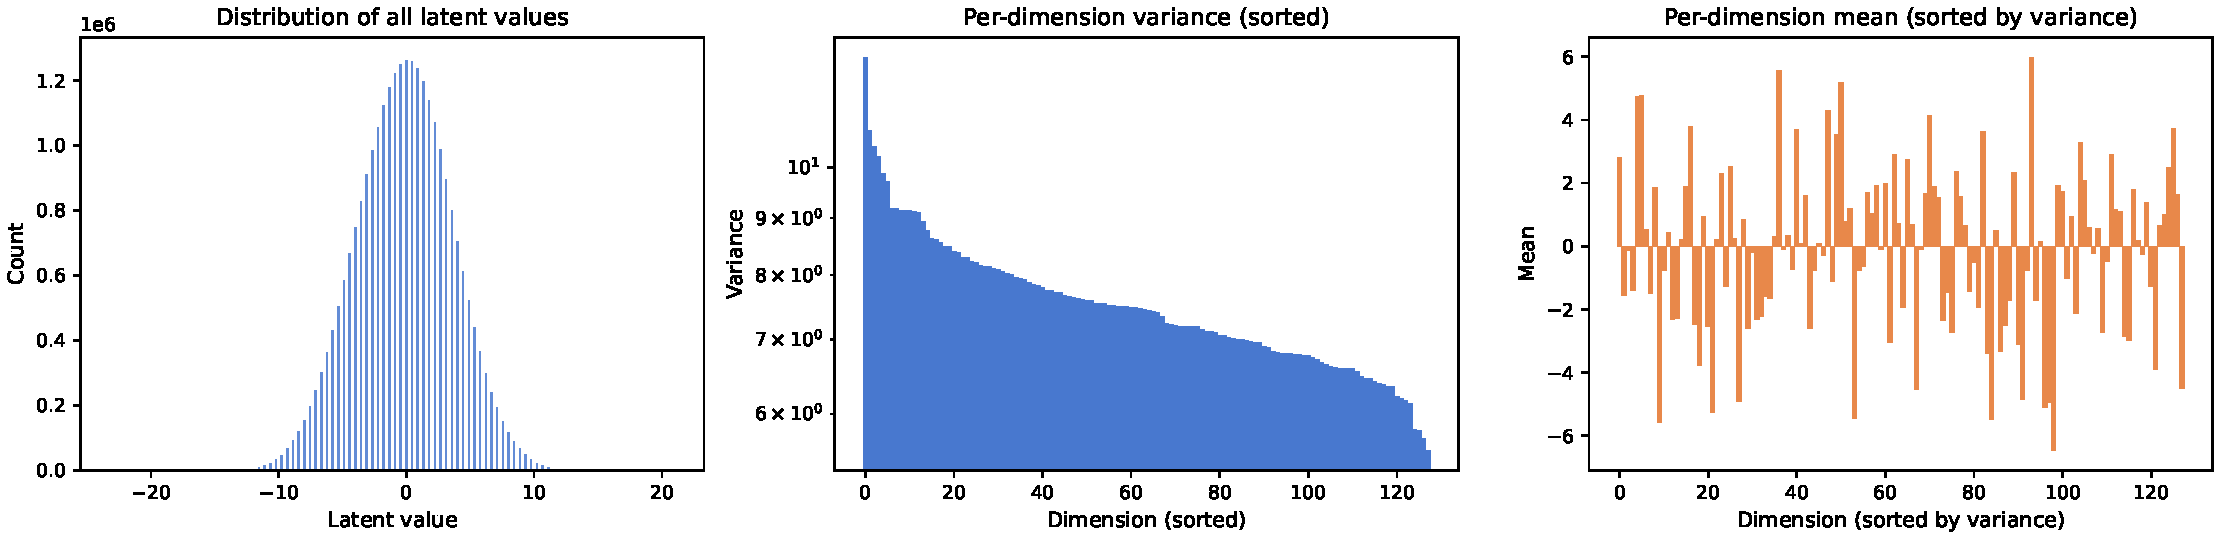
\includegraphics[width=0.92\textwidth]{../figures/diagnostics/tfocsvm_latent_statistics_2015.pdf}
  \\[6pt]
  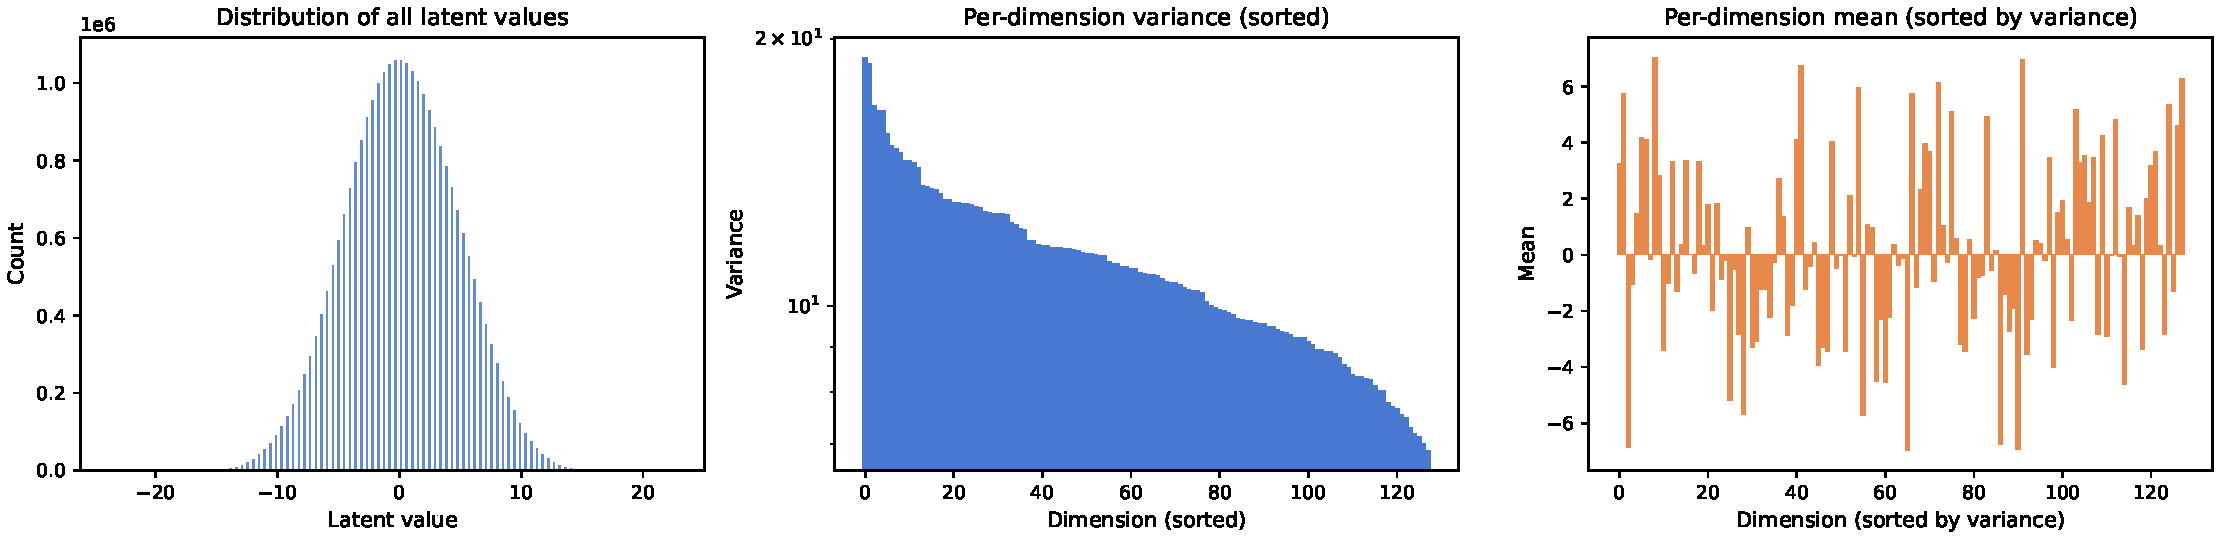
\includegraphics[width=0.92\textwidth]{../figures/diagnostics/tfocsvm_latent_statistics_2017.pdf}
  \caption{Per-dimension mean and variance of latent representations (top: 2015, bottom: 2017).}
  \label{fig:tfocsvm_latent}
\end{figure}

The Nystr\"om approximation to the RBF kernel uses 300 landmarks. Pairwise kernel values among a random subsample of latent vectors concentrate in $(0, 0.1)$, confirming that $\gamma$ places the operating point in a discriminative region rather than collapsing all similarities to~0 or to~1 (Figure~\ref{fig:tfocsvm_kernel}). The eigenvalue spectrum of the landmark kernel matrix decays rapidly, with an effective rank (95\% cumulative variance) well below 300, indicating that the landmark set captures the dominant structure efficiently (Figure~\ref{fig:tfocsvm_nystrom}).

\begin{figure}[H]
  \centering
  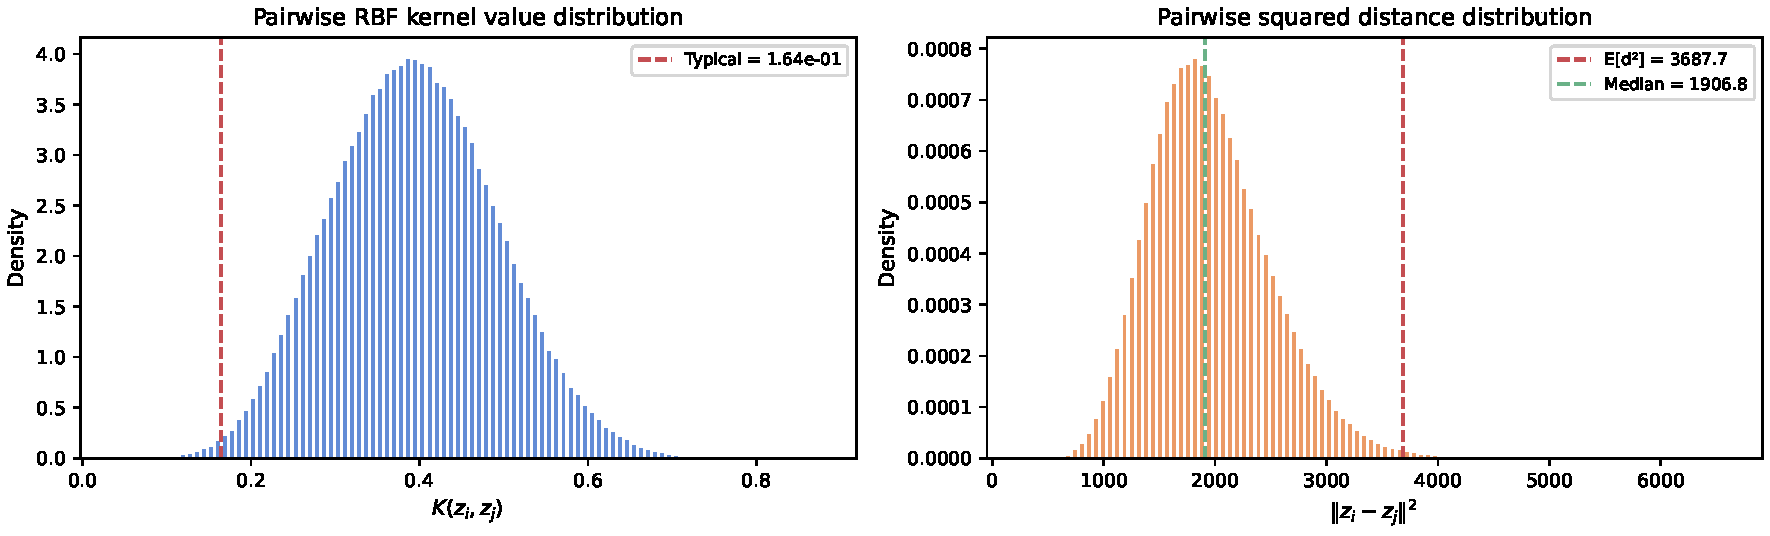
\includegraphics[width=0.92\textwidth]{../figures/diagnostics/tfocsvm_kernel_calibration_2015.pdf}
  \\[6pt]
  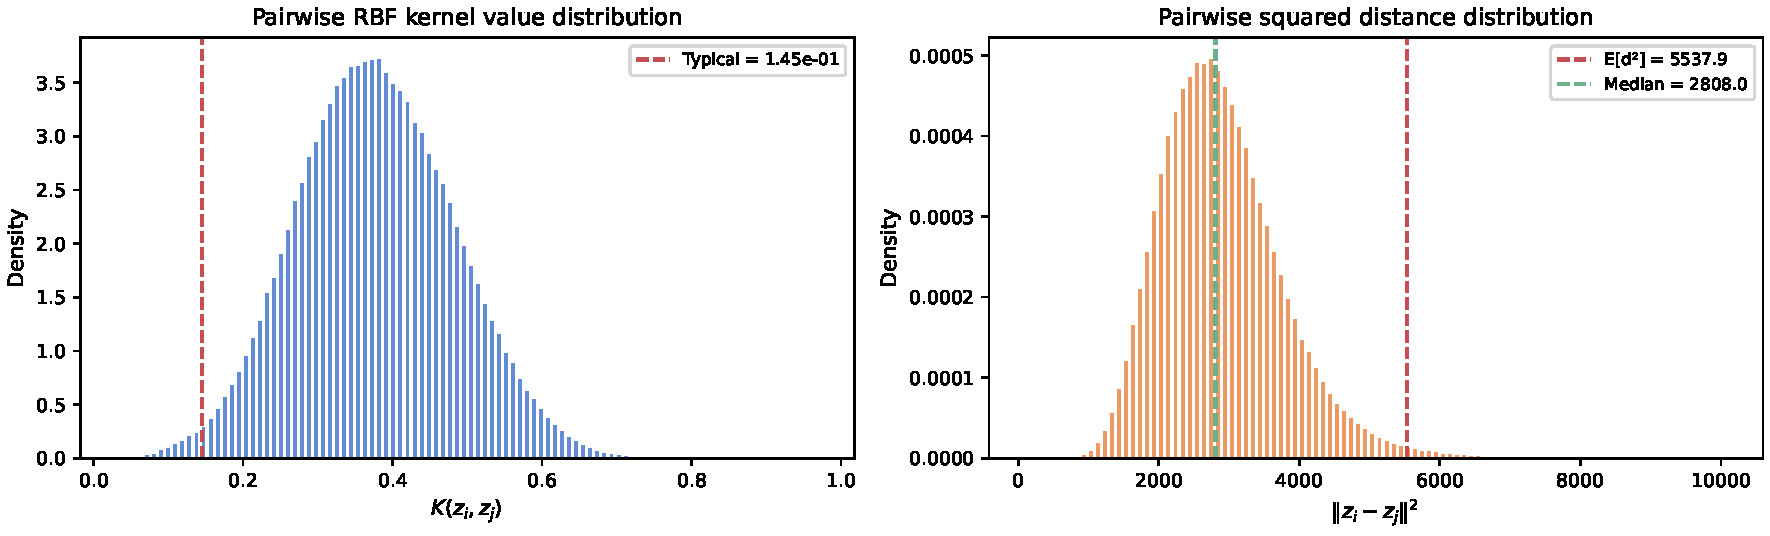
\includegraphics[width=0.92\textwidth]{../figures/diagnostics/tfocsvm_kernel_calibration_2017.pdf}
  \caption{Pairwise RBF kernel value distribution (top: 2015, bottom: 2017).}
  \label{fig:tfocsvm_kernel}
\end{figure}

\begin{figure}[H]
  \centering
  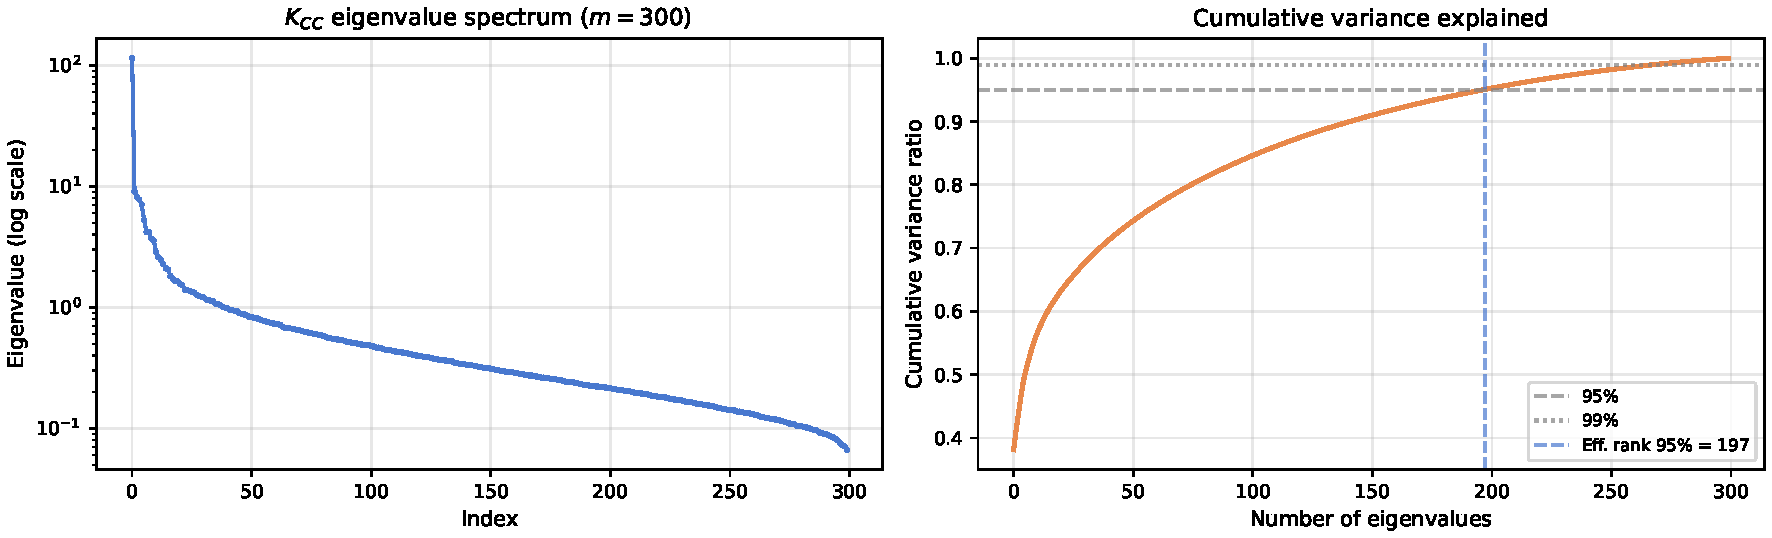
\includegraphics[width=0.92\textwidth]{../figures/diagnostics/tfocsvm_nystrom_spectrum_2015.pdf}
  \\[6pt]
  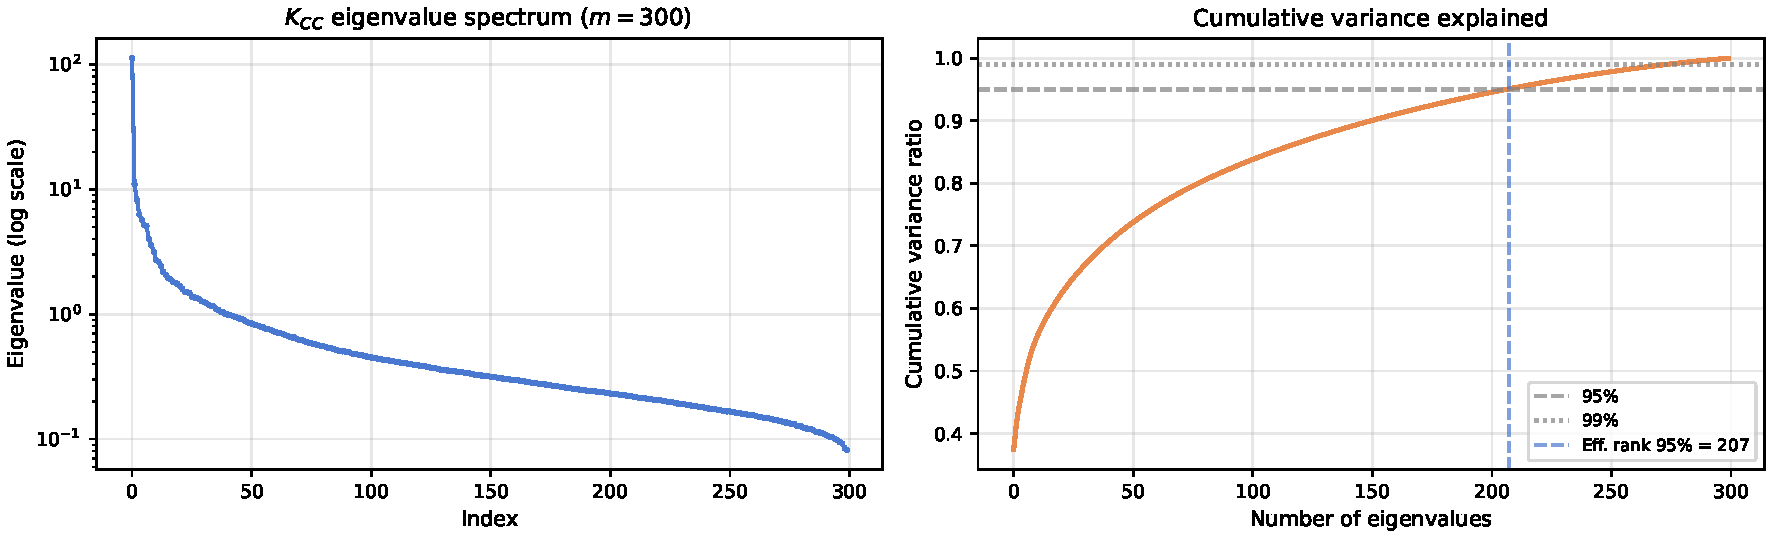
\includegraphics[width=0.92\textwidth]{../figures/diagnostics/tfocsvm_nystrom_spectrum_2017.pdf}
  \caption{Nystr\"om eigenvalue spectrum (top: 2015, bottom: 2017).}
  \label{fig:tfocsvm_nystrom}
\end{figure}

The distribution of the OC-SVM decision function $f(z) = \langle w, \Phi(z) \rangle - \rho$ on a representative test day concentrates at $f(z) > 0$ (inliers); the remaining fraction with $f(z) < 0$ constitutes the raw OC-SVM outlier set before any threshold adjustment (Figure~\ref{fig:tfocsvm_decision}).

\begin{figure}[H]
  \centering
  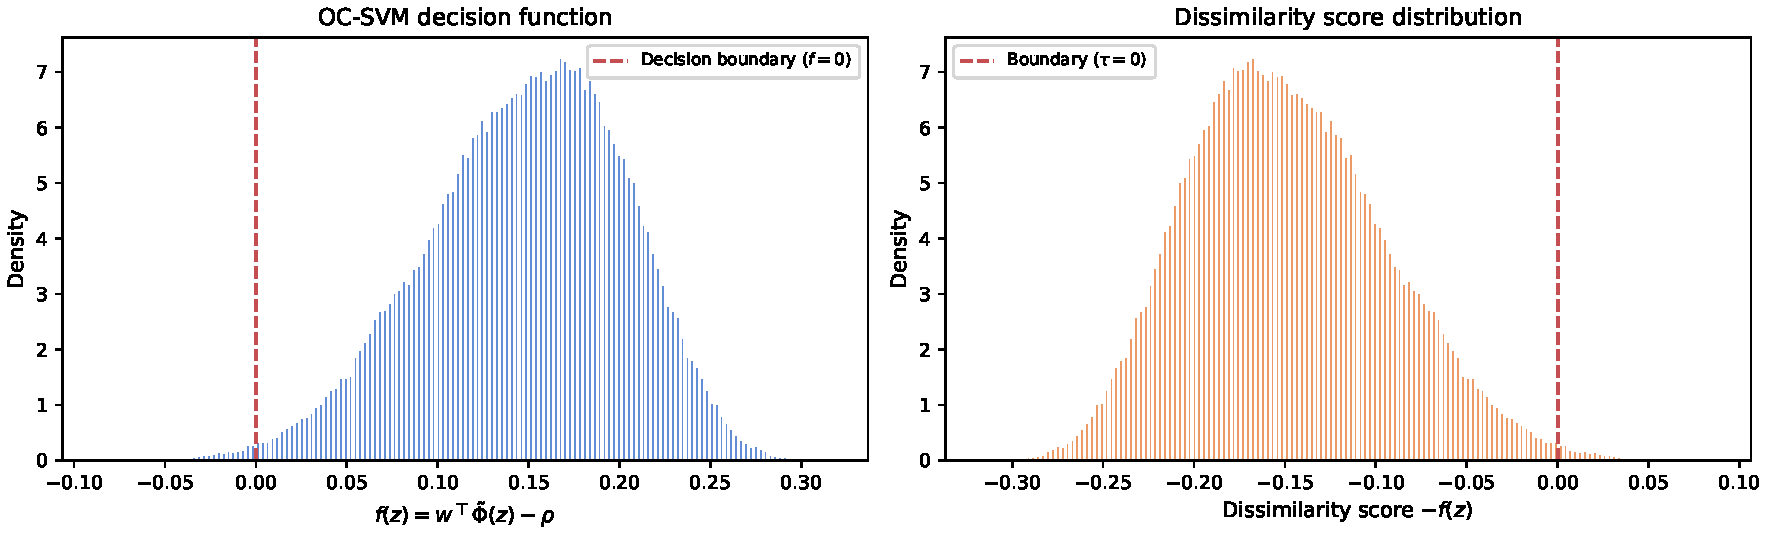
\includegraphics[width=0.92\textwidth]{../figures/diagnostics/tfocsvm_decision_function_2015.pdf}
  \\[6pt]
  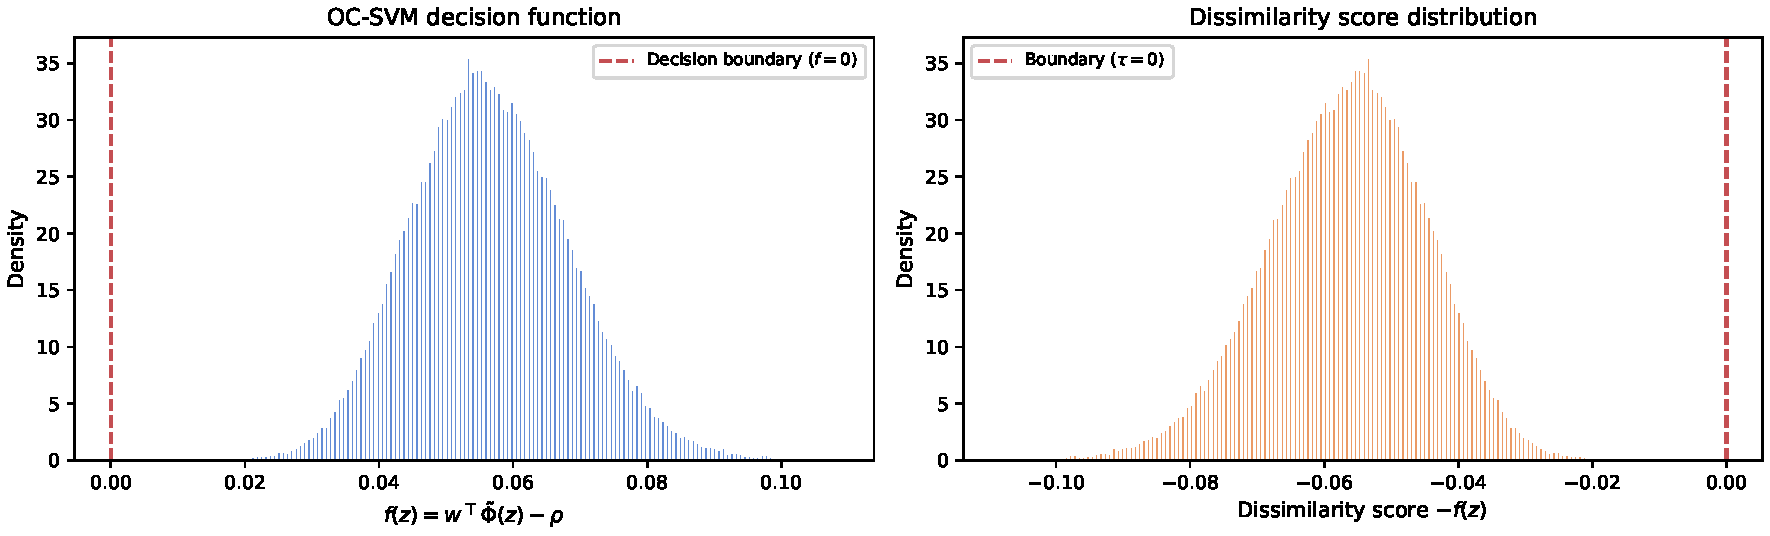
\includegraphics[width=0.92\textwidth]{../figures/diagnostics/tfocsvm_decision_function_2017.pdf}
  \caption{OC-SVM decision function distribution on a test day (top: 2015 model, bottom: 2017 model).}
  \label{fig:tfocsvm_decision}
\end{figure}

The correlation between reconstruction error and dissimilarity score is weak (Pearson $r \approx -0.16$ for 2015), confirming that the two score components capture complementary aspects of anomalousness (Figure~\ref{fig:tfocsvm_rec_dissim}). A PCA projection of the 128-dimensional latent space to two dimensions reveals that inliers form a dense cluster while outliers scatter along the periphery (Figure~\ref{fig:tfocsvm_pca}).

\begin{figure}[H]
  \centering
  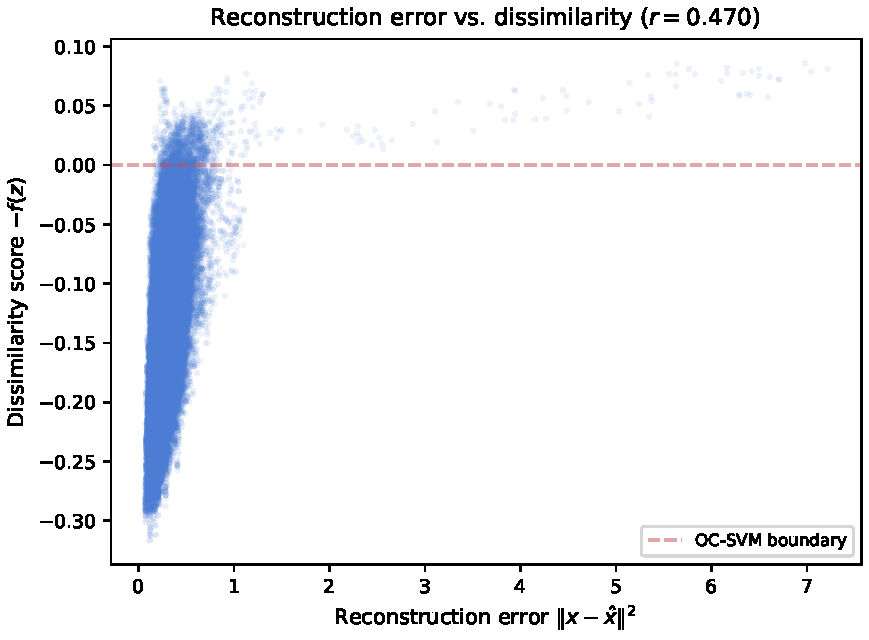
\includegraphics[width=0.92\textwidth]{../figures/diagnostics/tfocsvm_rec_vs_dissimilarity_2015.pdf}
  \\[6pt]
  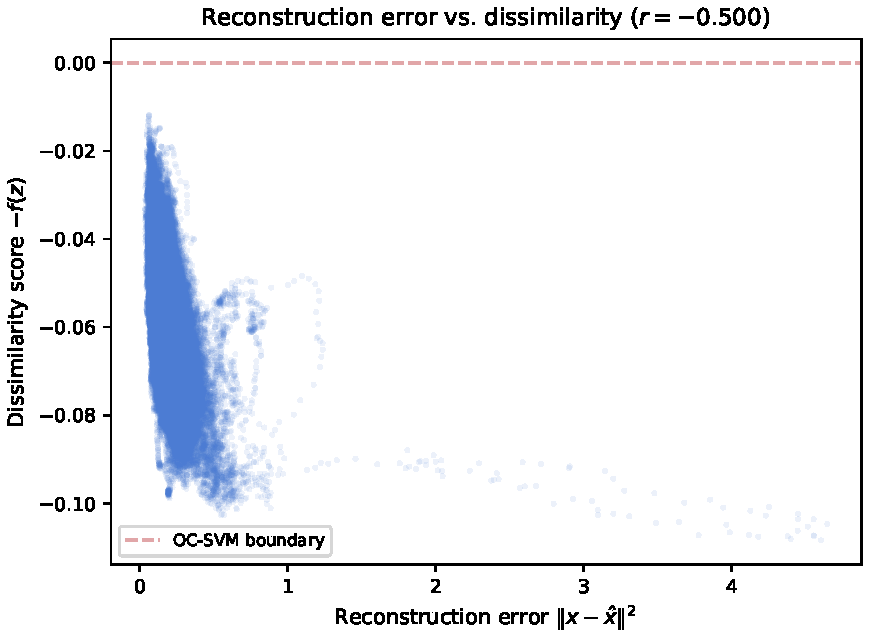
\includegraphics[width=0.92\textwidth]{../figures/diagnostics/tfocsvm_rec_vs_dissimilarity_2017.pdf}
  \caption{Reconstruction error vs.\ dissimilarity score (top: 2015, bottom: 2017).}
  \label{fig:tfocsvm_rec_dissim}
\end{figure}

\begin{figure}[H]
  \centering
  \includegraphics[width=0.92\textwidth]{../figures/diagnostics/tfocsvm_latent_pca_2015.pdf}
  \\[6pt]
  \includegraphics[width=0.92\textwidth]{../figures/diagnostics/tfocsvm_latent_pca_2017.pdf}
  \caption{PCA projection of the latent space; red marks outliers with $f < 0$ (top: 2015, bottom: 2017).}
  \label{fig:tfocsvm_pca}
\end{figure}

The baseline threshold~$\tau$ is fitted as the $(1-\nu)$-quantile of training dissimilarity scores, with $\nu = 0.01$. For the 2015 model, $\tau_{2015} = -0.019$ (computed from 288\,929 training scores), which sits below the OC-SVM boundary $f = 0$ and therefore produces a liberal detection regime that flags both clear outliers and boundary samples. The 2017 model yields $\tau_{2017} \approx -0.001$ (57\,153 scores), a near-zero threshold closer to the decision boundary. The training and test score distributions, superposed with the fitted~$\tau$ and the detection-rate curve as a function of the threshold, are presented in Figure~\ref{fig:tfocsvm_tau}.

\begin{figure}[H]
  \centering
  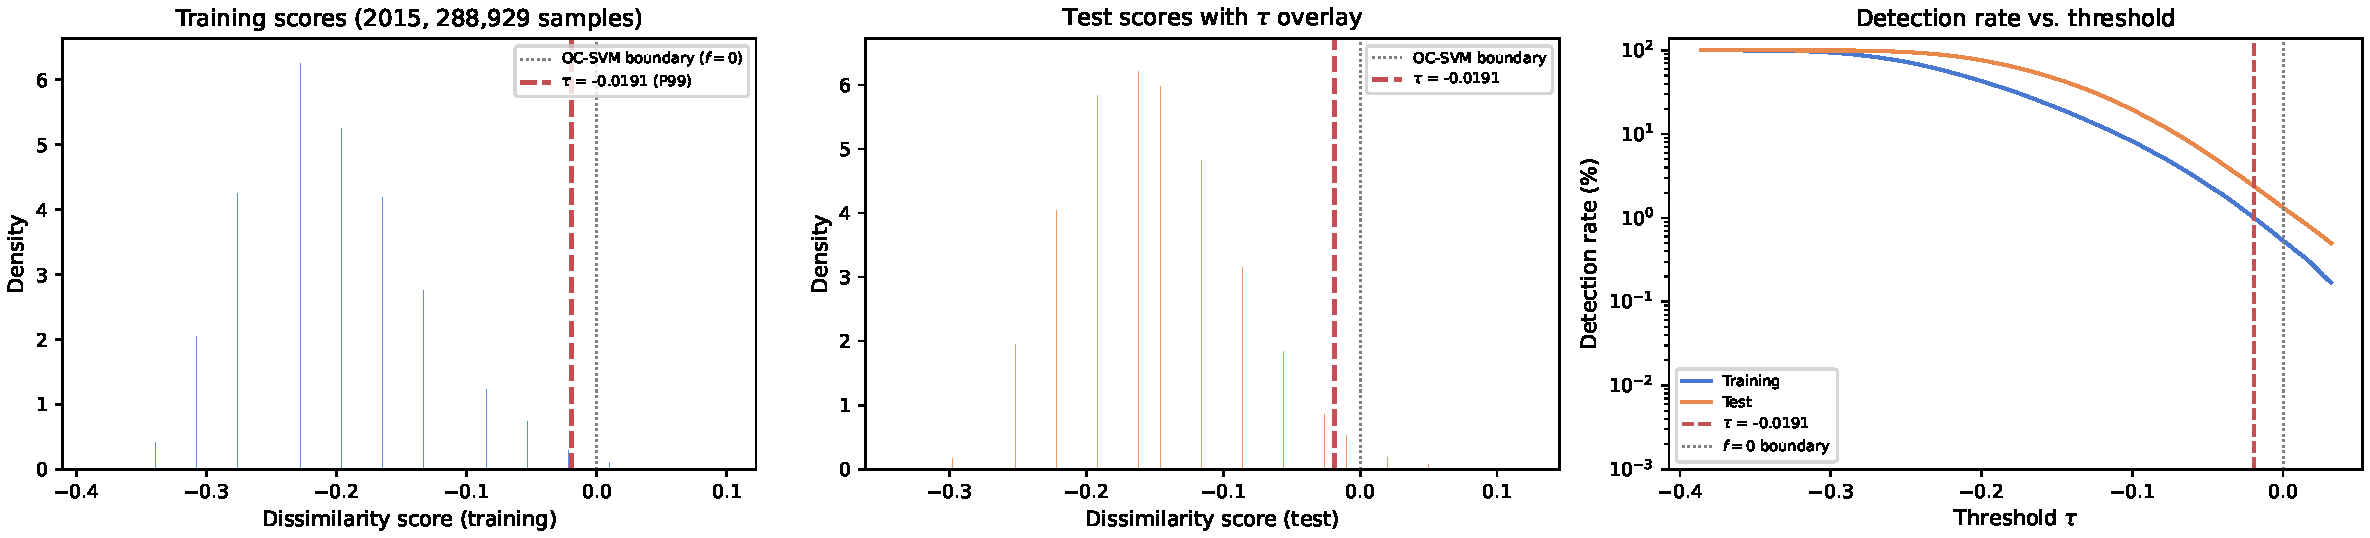
\includegraphics[width=0.92\textwidth]{../figures/diagnostics/tfocsvm_tau_analysis_2015.pdf}
  \\[6pt]
  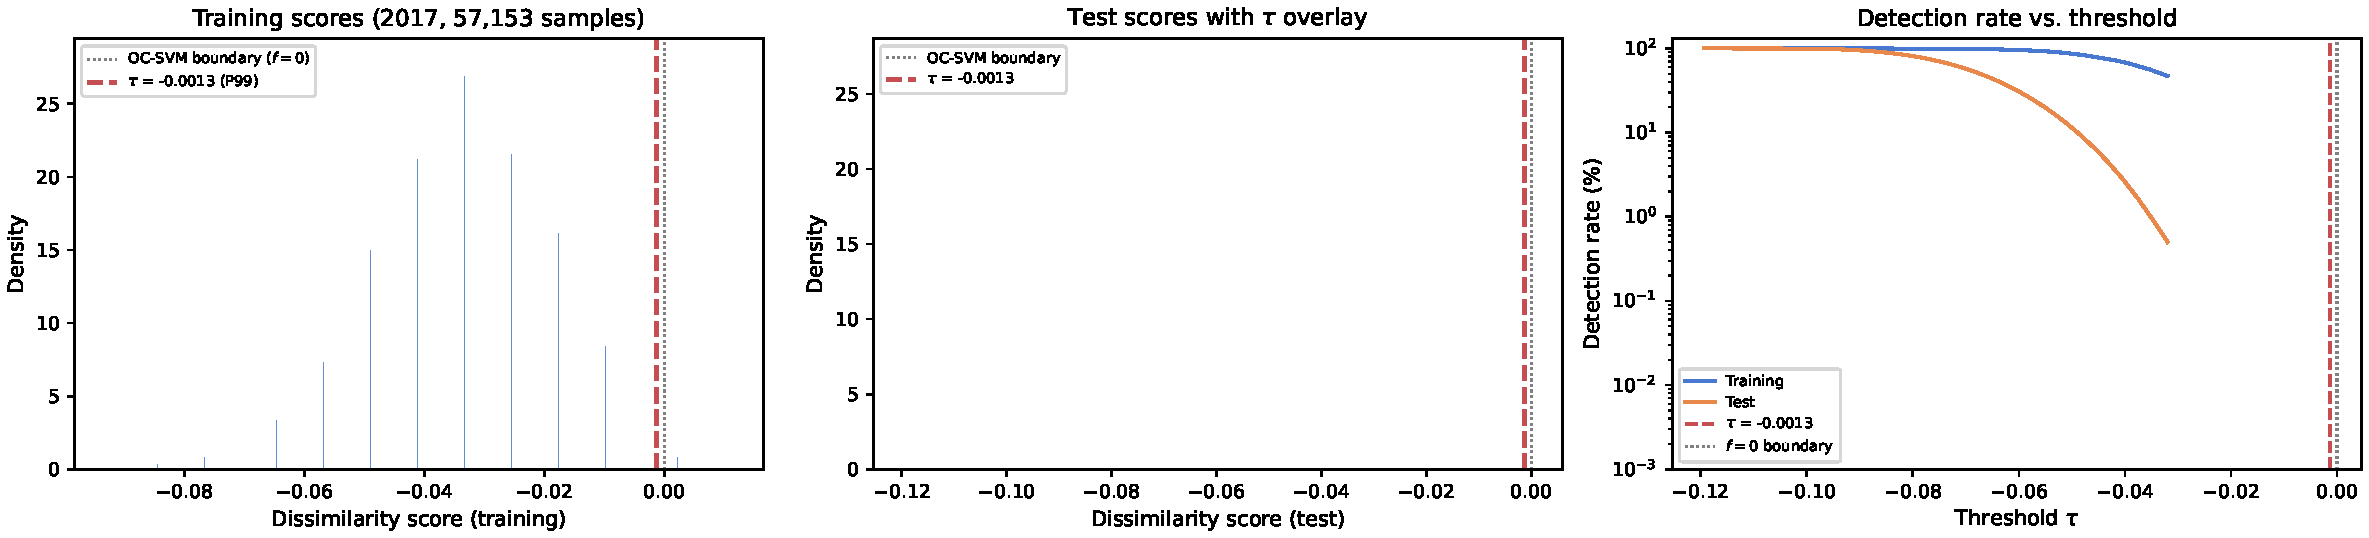
\includegraphics[width=0.92\textwidth]{../figures/diagnostics/tfocsvm_tau_analysis_2017.pdf}
  \caption{Threshold $\tau$ analysis: training/test score distributions and detection-rate curve (top: 2015, bottom: 2017).}
  \label{fig:tfocsvm_tau}
\end{figure}

\paragraph{Comparison across years.}
The 2015 model exhibits higher baseline reconstruction error than the 2017 model (mean 0.27 vs.\ 0.17), indicating that the encoder-decoder pair trained on 2015 data reconstructs its own training distribution less tightly. The 2017 bottleneck makes more structured use of the 128 latent dimensions: the first two PCA components capture 17.8\% of the total variance (10.0\% + 7.7\%), compared with 10.2\% (5.5\% + 4.6\%) for 2015 (Figure~\ref{fig:tfocsvm_pca}). The most prominent difference lies in the baseline threshold: $\tau_{2015} = -0.010$ flags 0.21\% of test events as anomalous, while $\tau_{2017} = -0.002$ flags 0.045\%, a factor of 4.7 (Figure~\ref{fig:tfocsvm_tau}). This gap originates in the different training-score distributions from which the $P_{99}$ quantile is drawn and will directly translate into a higher raw anomaly count for the 2015-trained model in Section~\ref{sec:results:detection}.

\subsection{Probabilistic Neural Network}\label{sec:results:diag:pnn}

The PNN outputs three per-event parameters of a skew-normal distribution: location~$\mu$, scale~$\sigma$, and shape~$\alpha$. The marginal distributions of these parameters on the test set (213\,138 events) indicate that the predicted~$\mu$ centres tightly around zero, consistent with near-zero mid-price returns at the LOB event scale (Figure~\ref{fig:pnn_params}). The scale~$\sigma$ remains strictly positive (minimum $\sim 10^{-4}$, enforced by the Softplus activation plus~$\varepsilon$), ruling out degenerate collapsed predictions. The skewness~$\alpha$ varies across events (standard deviation $\sim 1$), confirming that the network adapts the distribution shape per sample rather than learning a single global skew.

\begin{figure}[H]
  \centering
  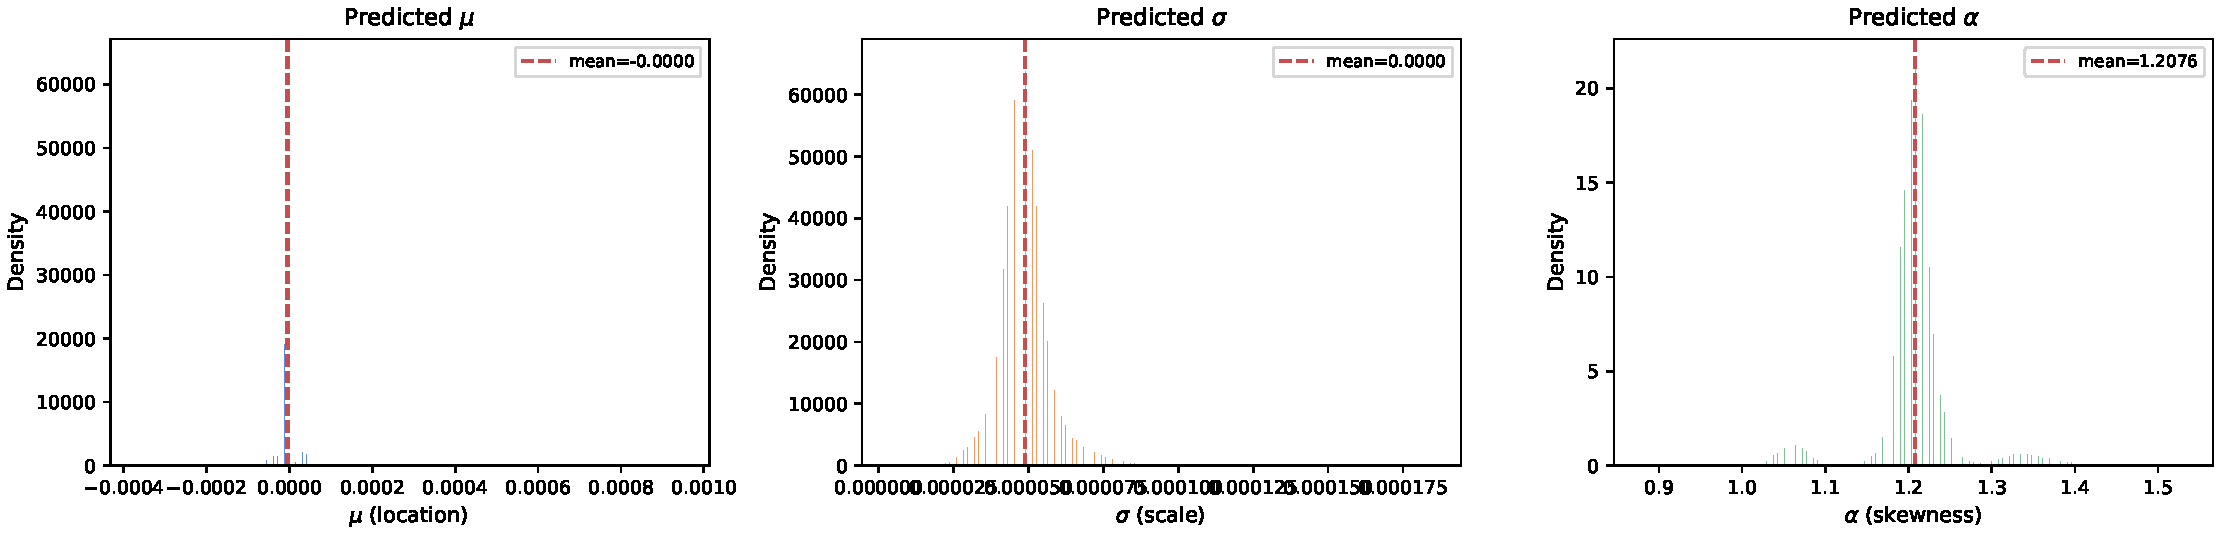
\includegraphics[width=0.92\textwidth]{../figures/diagnostics/pnn_parameters_2015.pdf}
  \\[6pt]
  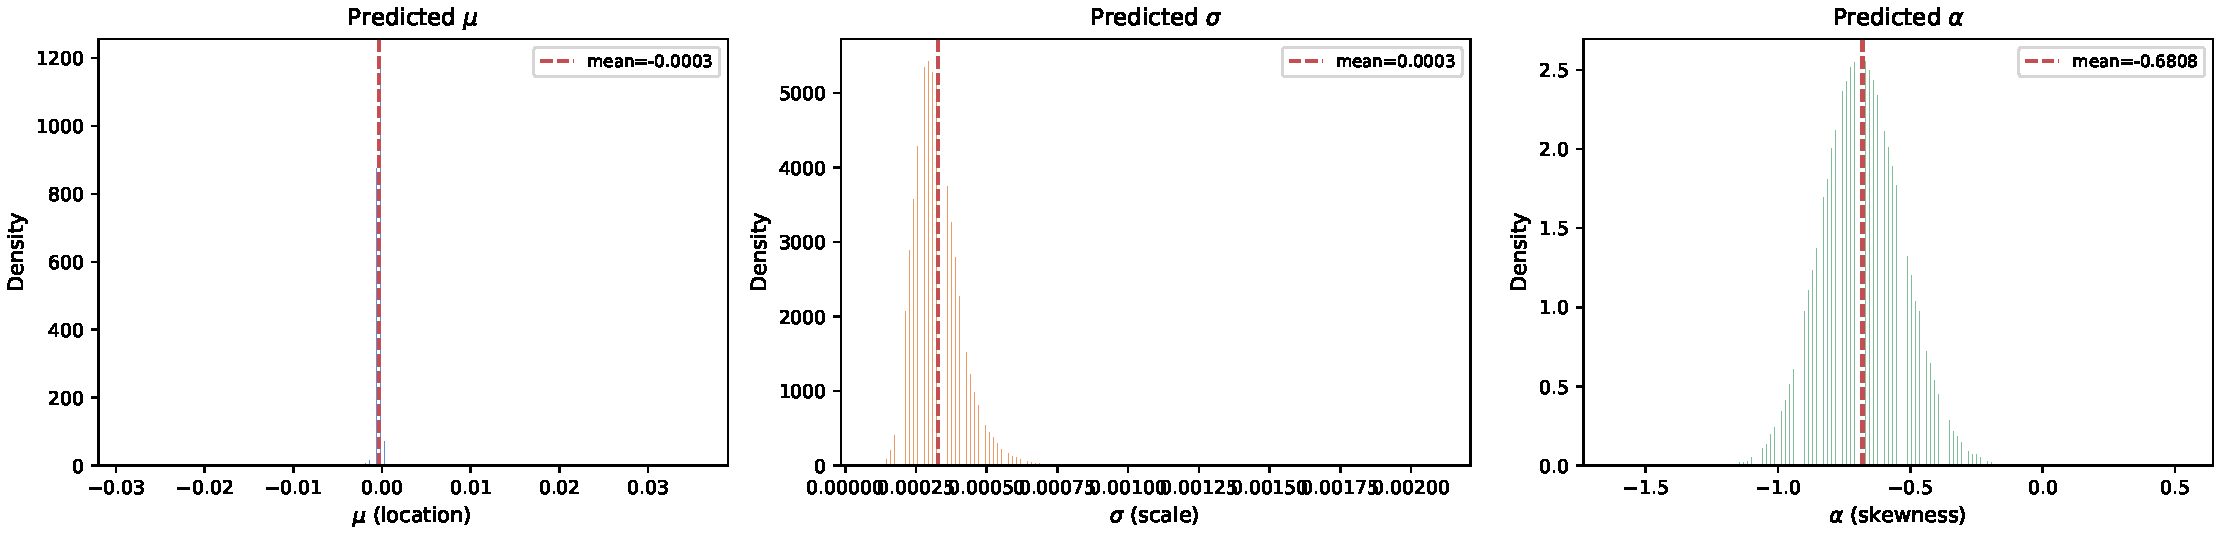
\includegraphics[width=0.92\textwidth]{../figures/diagnostics/pnn_parameters_2017.pdf}
  \caption{Predicted skew-normal parameters ($\mu$, $\sigma$, $\alpha$) on the test set (top: 2015, bottom: 2017).}
  \label{fig:pnn_params}
\end{figure}

The negative log-likelihood (NLL) serves as the anomaly score. The NLL distribution and its relationship with the predicted scale~$\sigma$ indicate that high NLL values correspond to events whose observed mid-price return lies far in the tails of the predicted skew-normal; these concentrate at low~$\sigma$, where the distribution is narrow and moderate deviations become unlikely (Figure~\ref{fig:pnn_nll}).

\begin{figure}[H]
  \centering
  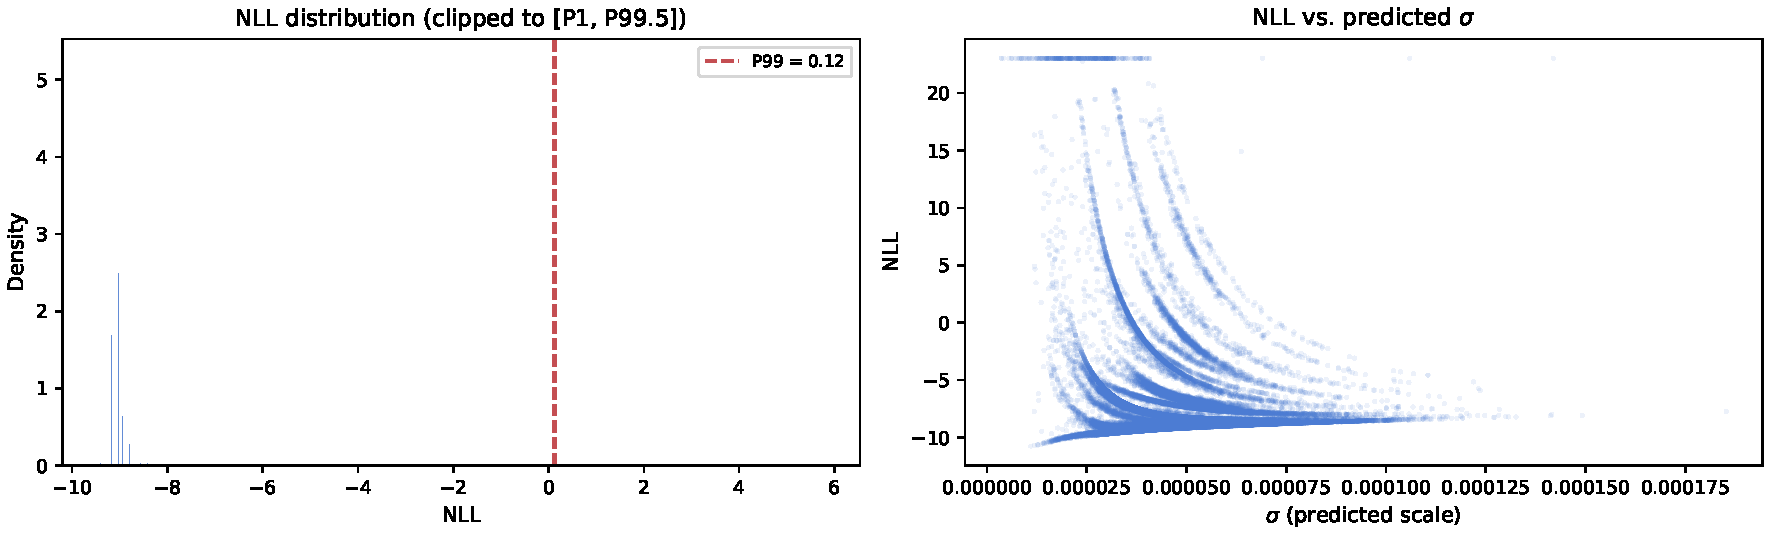
\includegraphics[width=0.92\textwidth]{../figures/diagnostics/pnn_nll_distribution_2015.pdf}
  \\[6pt]
  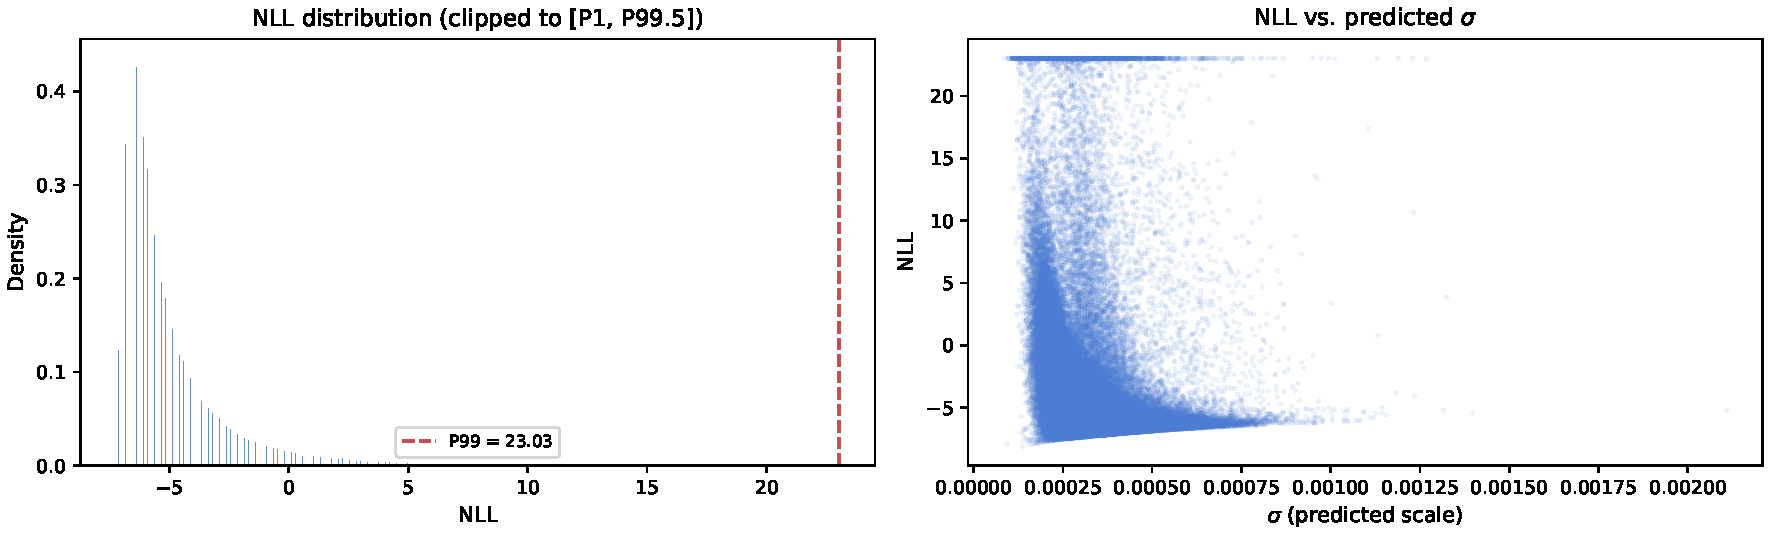
\includegraphics[width=0.92\textwidth]{../figures/diagnostics/pnn_nll_distribution_2017.pdf}
  \caption{NLL score distribution and NLL vs.\ predicted $\sigma$ (top: 2015, bottom: 2017).}
  \label{fig:pnn_nll}
\end{figure}

The spoofing gain $G_t$ measures the expected profit from a spoofing strategy under the PNN's predicted distribution (Section~\ref{sec:methodology:spoofing}). Computed on a 20\,000-event subsample with $\delta_a = 0$, $\delta_b = 0.01$\,EUR, $Q = 4{,}500$, $q = 100$, maker fee 0\%, taker fee 0.08\%, $G_t$ is negative for the majority of events (spoofing unprofitable); the fraction with $G_t > 0$ identifies potentially manipulable moments (Figure~\ref{fig:pnn_gain}).

\begin{figure}[H]
  \centering
  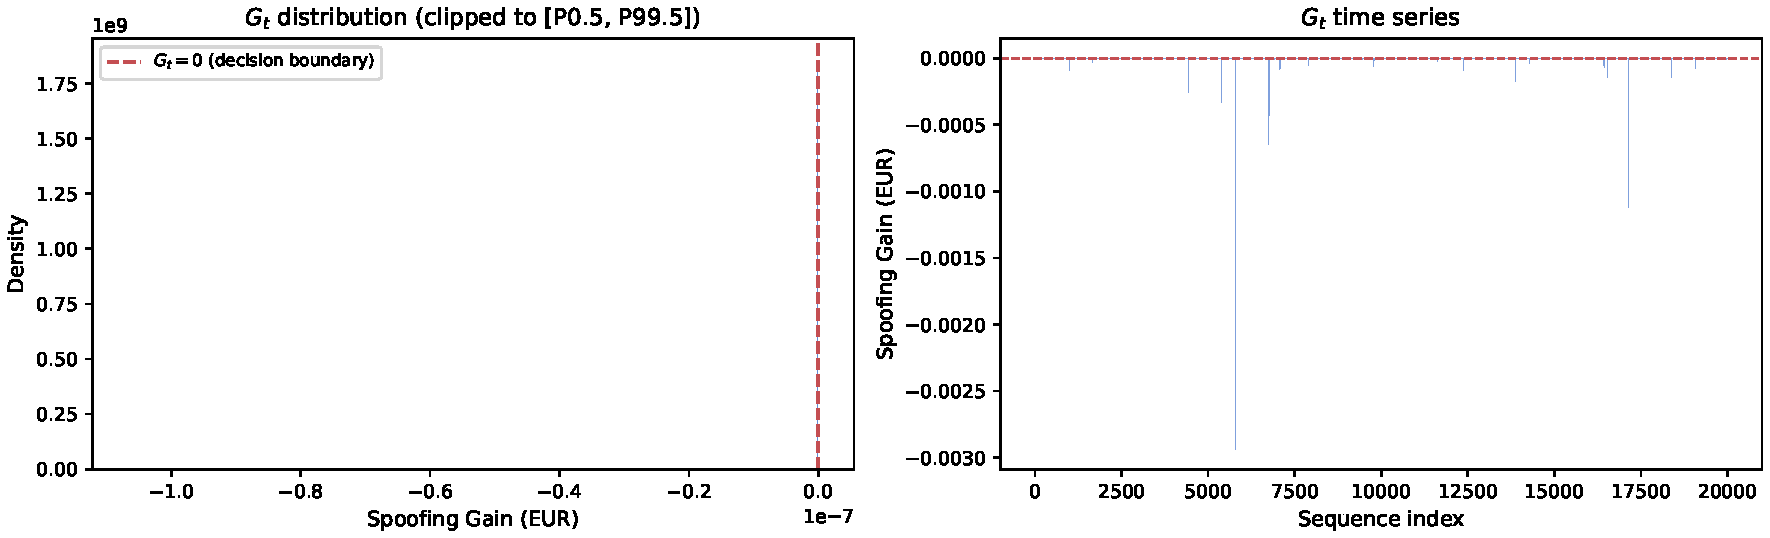
\includegraphics[width=0.92\textwidth]{../figures/diagnostics/pnn_gain_distribution_2015.pdf}
  \\[6pt]
  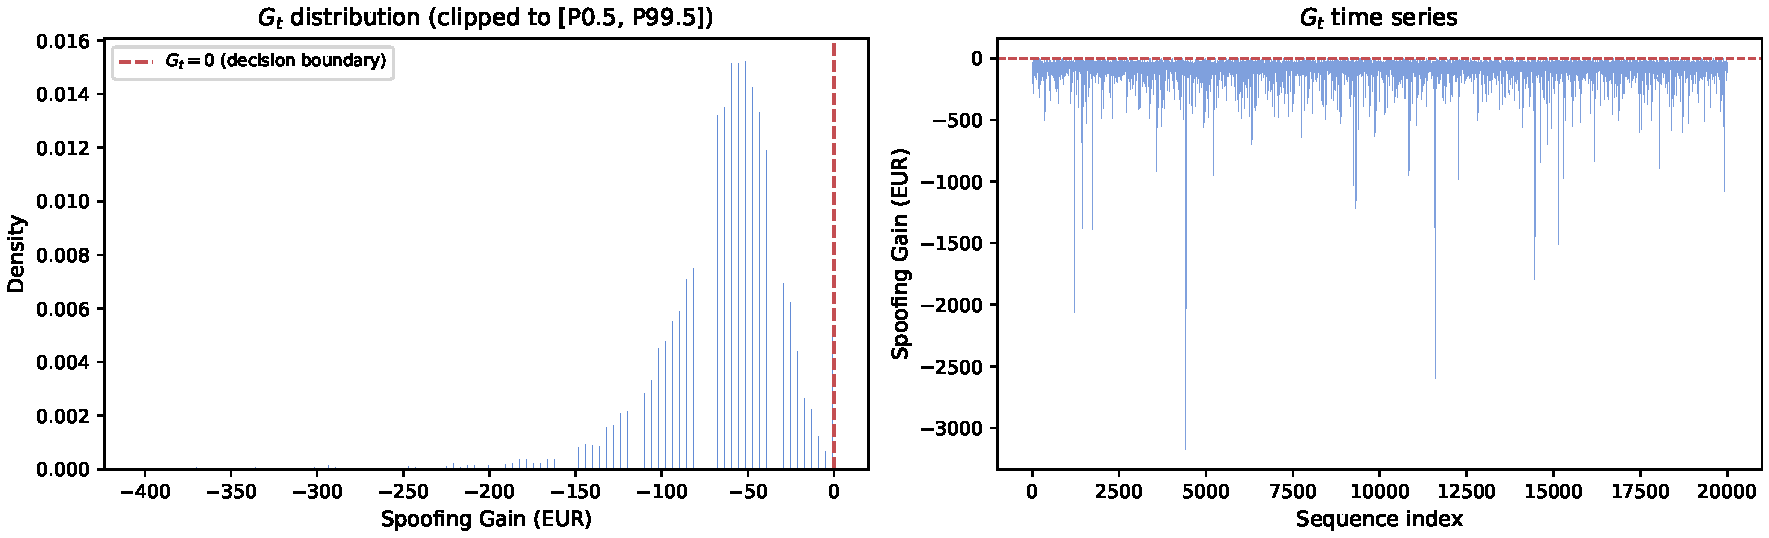
\includegraphics[width=0.92\textwidth]{../figures/diagnostics/pnn_gain_distribution_2017.pdf}
  \caption{Spoofing gain $G_t$ distribution and time series (top: 2015, bottom: 2017).}
  \label{fig:pnn_gain}
\end{figure}

A sweep of the spoof-order distance~$\delta_b$ from~0 to~0.05\,EUR reveals that both the mean $G_t$ and the percentage of events flagged ($G_t > 0$) decrease monotonically with~$\delta_b$ (Figure~\ref{fig:pnn_delta}): placing the spoofing order further from the best bid reduces its price-impact effect and therefore the expected profit, consistent with the analytical predictions of the model.

\begin{figure}[H]
  \centering
  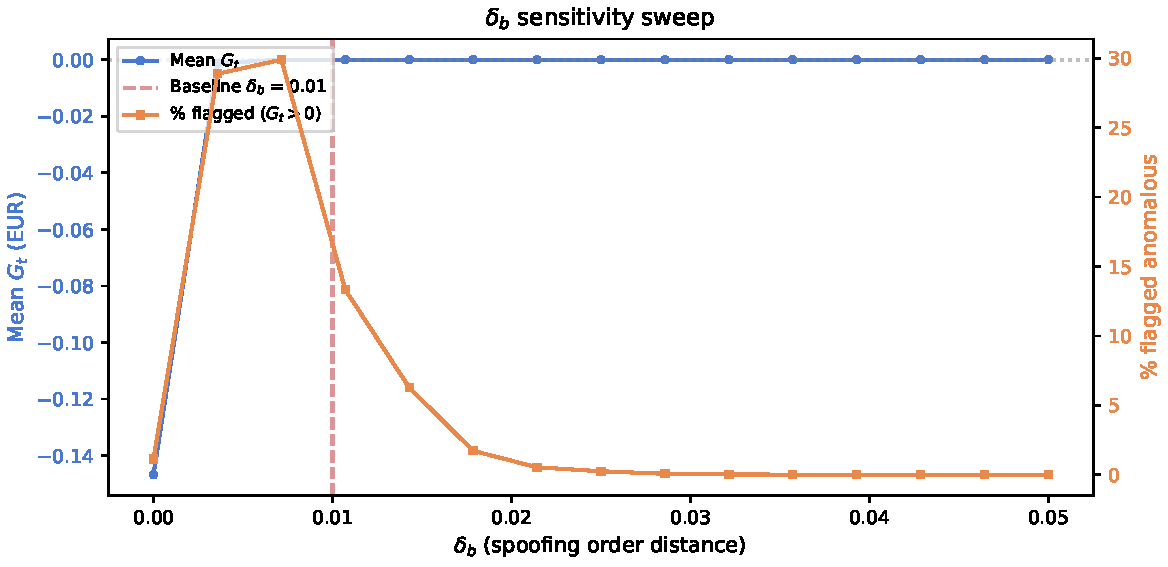
\includegraphics[width=0.92\textwidth]{../figures/diagnostics/pnn_delta_b_sweep_2015.pdf}
  \\[6pt]
  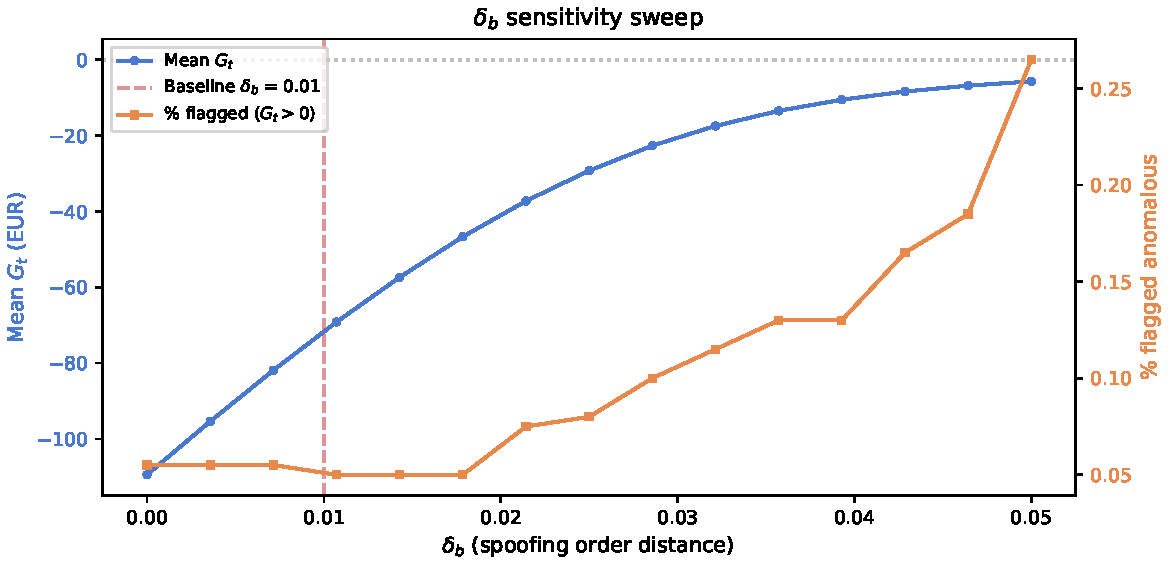
\includegraphics[width=0.92\textwidth]{../figures/diagnostics/pnn_delta_b_sweep_2017.pdf}
  \caption{$\delta_b$ sensitivity: mean $G_t$ and flag rate as a function of spoof-order distance (top: 2015, bottom: 2017).}
  \label{fig:pnn_delta}
\end{figure}

\paragraph{Comparison across years.}
The 2015 and 2017 PNN models produce qualitatively different predicted distributions. The 2015 model predicts a mean scale $\bar{\sigma}_{2015} = 4.9 \times 10^{-5}$ with positive skewness ($\bar{\alpha}_{2015} = +1.21$), whereas the 2017 model outputs $\bar{\sigma}_{2017} = 3.3 \times 10^{-4}$ with negative skewness ($\bar{\alpha}_{2017} = -0.68$) (Figure~\ref{fig:pnn_params}). Because the 2015 model assigns much narrower predictive distributions, even small deviations in the observed return produce high NLL: the 99th-percentile NLL is 0.20 for 2015 versus 23.0 for 2017 (Figure~\ref{fig:pnn_nll}). The effect on the spoofing gain is pronounced: 15.1\% of test events produce $G_t > 0$ under the 2015 model, compared with 0.1\% under the 2017 model (Figure~\ref{fig:pnn_gain}). This 150-fold difference in flag rate implies that the two PNN models yield different volumes of spoofing alerts in Section~\ref{sec:results:detection}, independent of any threshold choice.

\subsection{Probabilistic Robust Autoencoder}\label{sec:results:diag:prae}

The PRAE learns a per-sample gate parameter~$\mu_i \in (0,1)$ during training. Samples with $\mu_i$ close to~1 are reconstructed faithfully (``gated in''), while those with $\mu_i$ near~0 are suppressed as likely anomalies. The distribution of~$\mu$ across the training set is concentrated in a narrow band for both the 2015 model (61\,877 training samples) and the 2017 model (15\,079 samples): all $\mu$ values cluster around~0.502 with standard deviation $< 0.001$ (Figure~\ref{fig:prae_mu}). No sample falls below the nominal anomaly threshold $\mu < 0.1$; the stochastic gate has effectively collapsed to a constant, treating every training event identically. This behaviour indicates that the $\ell_1$ regularisation weight $\lambda$ ($1109.2685$ for the 2015 model, $215.4125$ for the 2017 model) and noise level $\sigma = 0.5$ are insufficient to force the gate to discriminate, and the reconstructor achieves low loss while ignoring the gating mechanism.

\begin{figure}[H]
  \centering
  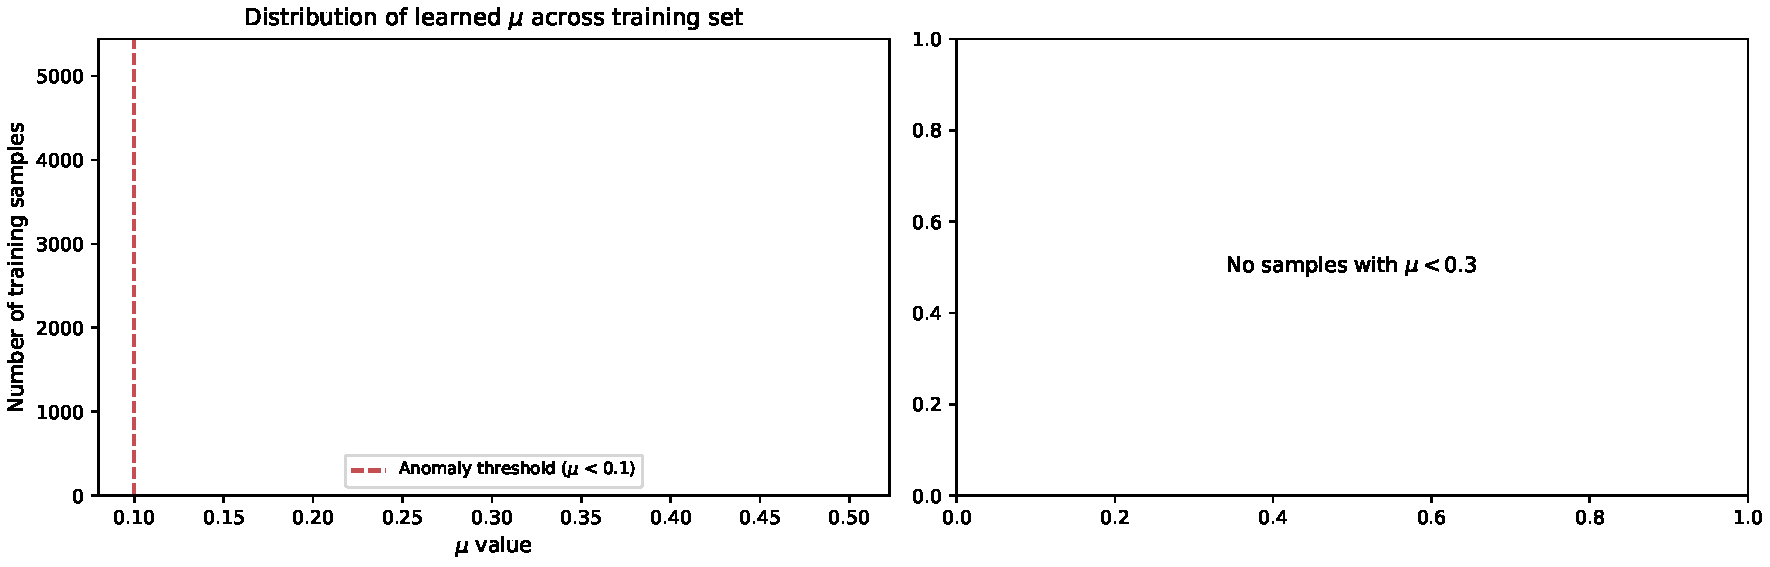
\includegraphics[width=0.92\textwidth]{../figures/diagnostics/prae_mu_distribution_2015.pdf}
  \\[6pt]
  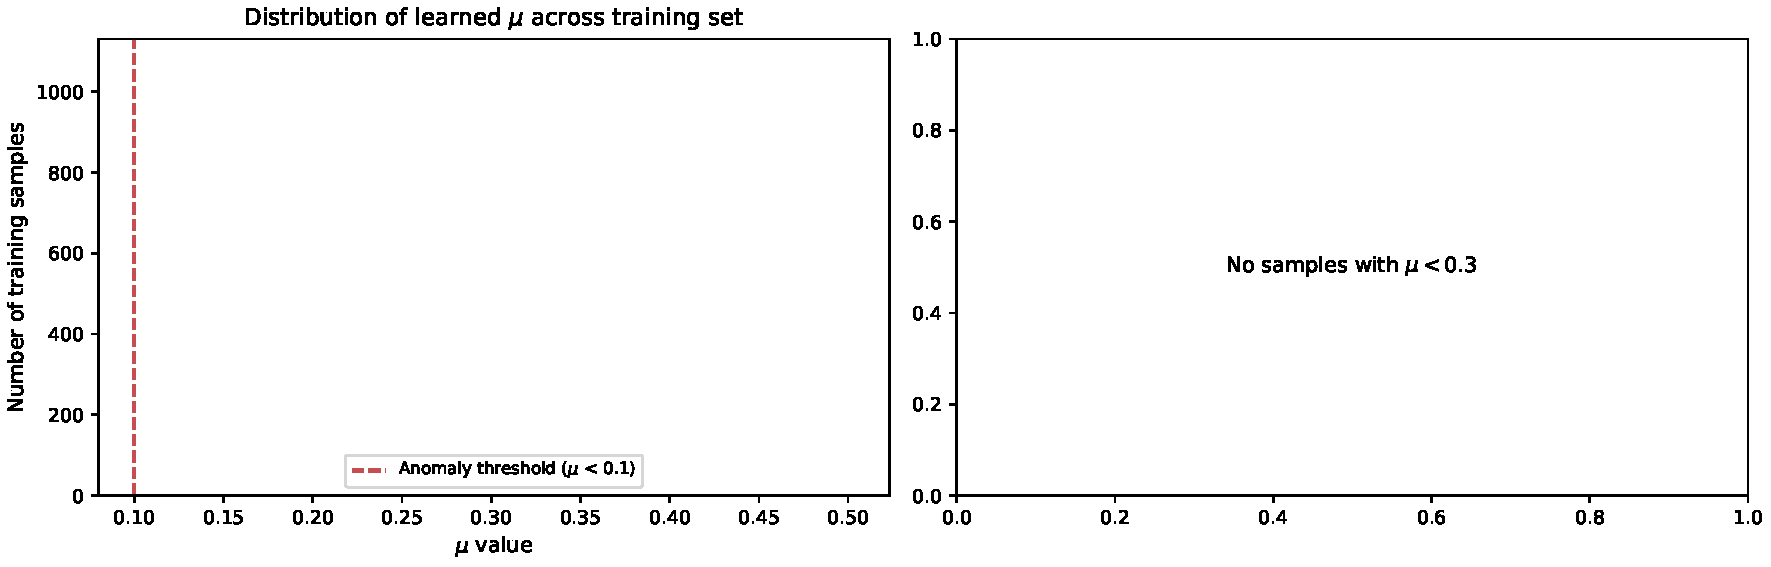
\includegraphics[width=0.92\textwidth]{../figures/diagnostics/prae_mu_distribution_2017.pdf}
  \caption{Distribution of learned gate parameters $\mu_i$ (top: 2015 model, bottom: 2017 model). The dashed line marks $\mu = 0.1$.}
  \label{fig:prae_mu}
\end{figure}

At test time, the PRAE score is the per-sample reconstruction error $\sum (x - \hat{x})^2$. The test-time score distribution is right-skewed: the bulk of events reconstruct well (low error), while a heavy tail extends to high reconstruction error, corresponding to events that deviate from the learned manifold of normal behaviour (Figure~\ref{fig:prae_score}).

\begin{figure}[H]
  \centering
  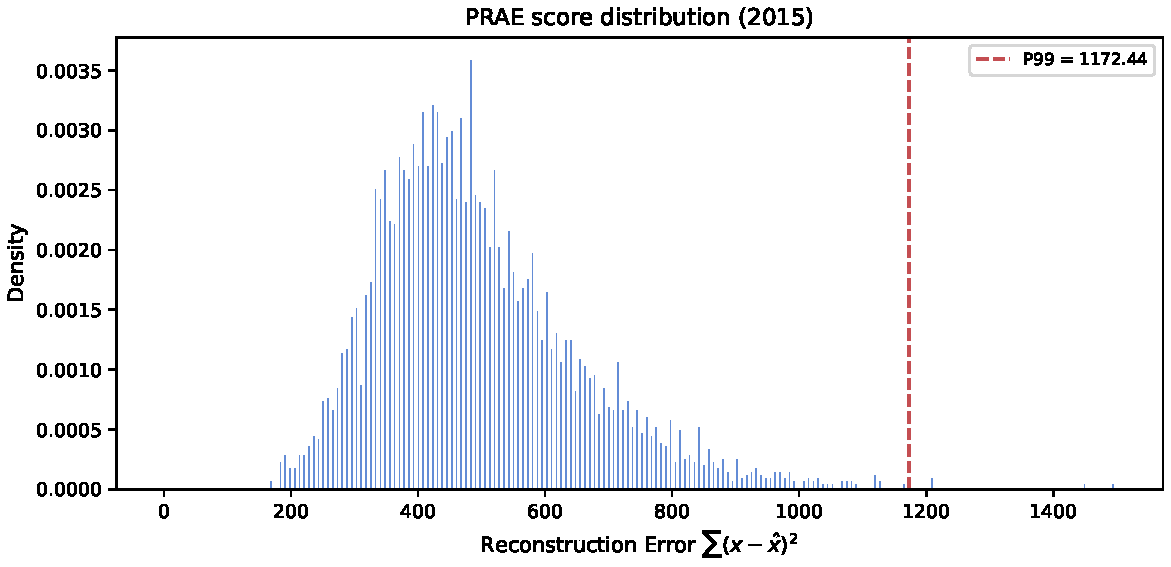
\includegraphics[width=0.92\textwidth]{../figures/diagnostics/prae_score_distribution_2015.pdf}
  \\[6pt]
  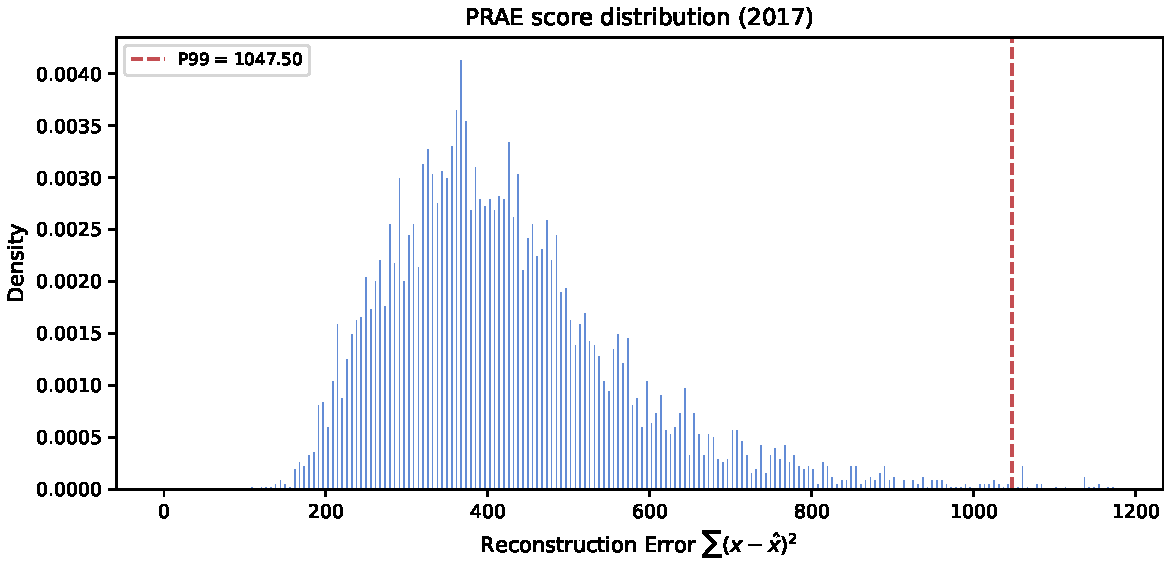
\includegraphics[width=0.92\textwidth]{../figures/diagnostics/prae_score_distribution_2017.pdf}
  \caption{PRAE test-time reconstruction error distribution (top: 2015, bottom: 2017). The dashed line marks P99.}
  \label{fig:prae_score}
\end{figure}

\paragraph{Comparison across years.}
The gate collapse is identical in both years. The 2015 model concentrates all 61\,877 training $\mu_i$ values at $0.502 \pm 0.0005$; the 2017 model concentrates its 15\,079 values at $0.502 \pm 0.0004$ (Figure~\ref{fig:prae_mu}). The automatically selected regularisation weight differs by a factor of 5.2 ($\lambda_{2015} = 1109$ vs.\ $\lambda_{2017} = 215$), yet neither value induces discriminative gating; both models reduce to standard autoencoders whose anomaly score is the reconstruction error alone. Because the gating mechanism is inoperative, any difference in detection rates between years will reflect only the distribution of reconstruction errors relative to the chosen threshold, not a difference in learned anomaly structure.


\section{Anomaly Detection on Test Data}\label{sec:results:detection}

Each model trained in Section~\ref{sec:results:diagnostics} is evaluated on the full multi-year test set. The 2015-trained pipeline scores 343~trading days (approximately 109~million LOB snapshots); the 2017-trained pipeline scores 295~trading days (approximately 99.7~million snapshots). Both test sets span January 2010 to April 2017 and are divided into three temporal splits: \emph{out-of-sample} (days that do not overlap with either training year), $\mathcal{T}_A$ (\emph{test-proximate}, 9~days adjacent to a training year), and $\mathcal{T}_B$ (\emph{test-distal}, 3~days far from any training year). Because the two pipelines are trained on different data partitions and produce distinct test outputs, both years' results are presented side by side.

\subsection{Anomaly Rates by Model and Time Period}\label{sec:results:detection:rates}

The aggregate anomaly rate for each model across four intraday periods, reported separately for the 2015-trained and 2017-trained pipelines in Table~\ref{tab:anomaly_period}, reveals distinct detection volumes between the two training years. The 2015-trained TF-OCSVM flags 2.0--2.8\% of windows (two orders of magnitude above the 2017 model's 0.00--0.03\%), the 2015 PNN flags 6.1--7.7\% (versus 0.06--0.08\% for 2017), and PRAE rates are comparable across years (2.2--3.7\% vs.\ 2.1--2.5\%). The large gap for TF-OCSVM and PNN reflects the diagnostic differences noted in Section~\ref{sec:results:diagnostics}: the 2015 TF-OCSVM operates with a more liberal baseline threshold ($\tau_{2015} = -0.019$ vs.\ $\tau_{2017} \approx -0.001$), and the 2015 PNN predicts much narrower distributions ($\bar\sigma_{2015} = 4.9 \times 10^{-5}$), causing even routine price moves to produce high NLL scores.

\begin{table}[H]
\centering
\caption{Anomaly rate (\%) by model and intraday period.  Left block:
2015-trained models; right block: 2017-trained models.}
\label{tab:anomaly_period}
\small
\begin{tabular}{l ccc ccc}
\toprule
& \multicolumn{3}{c}{\textbf{2015 model}} & \multicolumn{3}{c}{\textbf{2017 model}} \\
\cmidrule(lr){2-4}\cmidrule(lr){5-7}
Period & TF-OCSVM & PNN & PRAE & TF-OCSVM & PNN & PRAE \\
\midrule
First hour        & 2.709 & 7.037 & 2.162 & 0.020 & 0.063 & 2.068 \\
Rest of morning   & 2.454 & 6.362 & 2.246 & 0.019 & 0.065 & 2.113 \\
Afternoon         & 1.972 & 6.132 & 2.612 & 0.033 & 0.068 & 2.148 \\
US open           & 2.769 & 7.692 & 3.660 & 0.000 & 0.076 & 2.453 \\
\bottomrule
\end{tabular}
\end{table}

All three models exhibit a mild increase toward the afternoon and US~open sessions under both training years. For PRAE, the US~open rate exceeds the morning rate by roughly 20\% (2017 model) to 70\% (2015 model), consistent with the higher volatility typically observed around 15:30~CET. The 2017 TF-OCSVM produces zero anomalies during the US~open, suggesting that its OC-SVM boundary is calibrated more conservatively for that regime; the 2015 model, by contrast, flags 2.8\% of US~open windows, indicating a fundamentally different operating point.

\begin{figure}[H]
\centering
\includegraphics[width=0.85\linewidth]{../figures/results/anomaly_rates_by_period_2015.pdf}
\\[6pt]
\includegraphics[width=0.85\linewidth]{../figures/results/anomaly_rates_by_period_2017.pdf}
\caption{Anomaly rate by intraday period for each model (top: 2015 model, bottom: 2017 model).}
\label{fig:anomaly_rates_period}
\end{figure}

Daily anomaly rates for each model over the full test period are plotted separately for the 2015 and 2017 models in Figure~\ref{fig:daily_rates}. Out-of-sample days (gray) cluster tightly around each model's mean rate under the 2017 model but span a wider band under the 2015 model. The nine $\mathcal{T}_A$ days (red) and three $\mathcal{T}_B$ days (purple) are highlighted; their rates are analysed in Section~\ref{sec:results:detection:agreement}.

\begin{figure}[H]
\centering
\includegraphics[width=\linewidth]{../figures/results/daily_anomaly_rates_2015.pdf}
\\[6pt]
\includegraphics[width=\linewidth]{../figures/results/daily_anomaly_rates_2017.pdf}
\caption{Daily anomaly rate across the test period (top: 2015 model, bottom: 2017 model). The 10-day moving average is computed over out-of-sample days only. $\mathcal{T}_A$ and $\mathcal{T}_B$ days are coloured separately.}
\label{fig:daily_rates}
\end{figure}

The mean daily rate in each split, summarised as a heatmap for both training years, reveals that under the 2017 model PRAE dominates the colour scale in every split, whereas under the 2015 model PNN produces the highest rates across all splits, followed by PRAE and TF-OCSVM (Figure~\ref{fig:rate_heatmap}).

\begin{figure}[H]
\centering
\includegraphics[width=0.6\linewidth]{../figures/results/rate_heatmap_2015.pdf}
\\[6pt]
\includegraphics[width=0.6\linewidth]{../figures/results/rate_heatmap_2017.pdf}
\caption{Mean daily anomaly rate (\%) by model and temporal split (top: 2015 model, bottom: 2017 model).}
\label{fig:rate_heatmap}
\end{figure}

\subsection{Score Time Series and Distributions}\label{sec:results:detection:timeseries}

The anomaly score (or prediction) for each model on a single proximate test day is presented in Figure~\ref{fig:score_ts} for the 2015 and 2017 models. Under the 2017 model, the TF-OCSVM decision score is continuously negative for normal windows, with sparse anomaly crossings; under the 2015 model, the score distribution shifts lower (mean $-0.158$ vs.\ $-0.061$), and detected events are more numerous. PNN outputs binary predictions; under the 2015 model, anomaly bursts are frequent (6--8\% rate), whereas the 2017 model flags under 0.1\%. PRAE reconstruction scores are qualitatively similar across years, with flagged anomalies concentrated at peaks.

\begin{figure}[H]
\centering
\includegraphics[width=\linewidth]{../figures/results/score_timeseries_2015.pdf}
\\[6pt]
\includegraphics[width=\linewidth]{../figures/results/score_timeseries_2017.pdf}
\caption{Score time series for a representative proximate test day (top: 2015 model, bottom: 2017 model). TF-OCSVM: continuous decision score (anomaly when $>0$). PNN: binary prediction (no continuous score). PRAE: reconstruction score (anomaly above a learned threshold).}
\label{fig:score_ts}
\end{figure}

The score distributions for the two models that produce continuous outputs are presented separately for each training year in Figure~\ref{fig:score_dist}. The 2015 TF-OCSVM distribution spans $[-0.42, 0.13]$ with a mean of $-0.158$, and 0.96\% of windows cross the zero threshold. The 2017 TF-OCSVM distribution is concentrated in $[-0.12, 0.02]$ with a mean of $-0.061$ and 0.025\% crossing zero. The PRAE distribution is right-skewed under both years, with a mean reconstruction score of 426.4 (2015) vs.\ 443.7 (2017).

\begin{figure}[H]
\centering
\includegraphics[width=0.9\linewidth]{../figures/results/score_distributions_2015.pdf}
\\[6pt]
\includegraphics[width=0.9\linewidth]{../figures/results/score_distributions_2017.pdf}
\caption{Score distributions on the full test set (top: 2015 model, bottom: 2017 model). Left: TF-OCSVM decision score (dashed line marks the zero threshold). Right: PRAE reconstruction score (clipped at the 99.5th percentile for legibility).}
\label{fig:score_dist}
\end{figure}

\subsection{Model Agreement and Proximity Analysis}\label{sec:results:detection:agreement}

The fraction of test windows on which zero, one, two, or all three models flag an anomaly differs between training years (Table~\ref{tab:consensus}). Under the 2017 model, 97.74\% of windows are normal by every model and no window is flagged by all three simultaneously. Under the 2015 model, 89.56\% of windows are unanimously normal; 9.59\% are flagged by exactly one model, 0.80\% by two, and 0.04\% (46\,609 windows) by all three. This constitutes a qualitative difference from the 2017 result, where triple agreement is absent, and reflects the higher detection volumes of the 2015 TF-OCSVM and PNN models, which create overlap with PRAE's broadly flagged set.

\begin{table}[H]
\centering
\caption{Consensus agreement: fraction of test windows flagged by
$k$ models ($k = 0, 1, 2, 3$).}
\label{tab:consensus}
\small
\begin{tabular}{c rr rr}
\toprule
& \multicolumn{2}{c}{\textbf{2015 model}} & \multicolumn{2}{c}{\textbf{2017 model}} \\
\cmidrule(lr){2-3}\cmidrule(lr){4-5}
Models & Count & \% & Count & \% \\
\midrule
0 & 97\,690\,611 & 89.56 & 97\,432\,235 & 97.74 \\
1 & 10\,465\,145 & 9.59  & 2\,245\,476  & 2.25  \\
2 & 875\,408     & 0.80  & 5\,229       & 0.005 \\
3 & 46\,609      & 0.04  & 0            & 0.000 \\
\bottomrule
\end{tabular}
\end{table}

\begin{figure}[H]
\centering
\includegraphics[width=0.9\linewidth]{../figures/results/consensus_agreement_2015.pdf}
\\[6pt]
\includegraphics[width=0.9\linewidth]{../figures/results/consensus_agreement_2017.pdf}
\caption{Consensus breakdown (top: 2015 model, bottom: 2017 model). Left: overall consensus (pie). Right: sample counts for anomalies detected by 1, 2, or 3 models (horizontal bar).}
\label{fig:consensus}
\end{figure}

Under the 2017 model, the 5\,229 two-model agreements almost exclusively involve PRAE plus one other model, consistent with PRAE having the highest base rate (2.17\%). Under the 2015 model, the 875\,408 two-model agreements are distributed more broadly because all three models flag a non-trivial fraction of windows. A majority-vote rule (at least two of three) would flag approximately 5\,200 windows under the 2017 model (composite rate 0.005\%) but 922\,017 windows under the 2015 model (composite rate 0.85\%).

\paragraph{Proximity analysis.}
Anomaly rates on $\mathcal{T}_A$ (9~proximate days) and $\mathcal{T}_B$ (3~distal days) are compared for each training year in Figure~\ref{fig:proximity}.

Under the 2017 model, TF-OCSVM shows similar rates in both splits (0.56\% vs.\ 0.51\%, $p = 0.64$). PNN likewise shows no significant difference (0.008\% vs.\ 0.012\%, $p = 0.60$). PRAE is the only model for which the proximate rate (1.37\%) significantly exceeds the distal rate (1.04\%), with a Welch $t$-statistic of 3.14 and $p = 0.014$.

Under the 2015 model, the pattern differs. TF-OC-SVM shows a higher proximate rate (2.65\%) than distal (0.73\%), though the difference does not reach significance ($p = 0.17$). PNN reverses the pattern: the distal rate (4.01\%) exceeds the proximate rate (2.60\%, $p = 0.10$). PRAE shows no significant proximity effect under the 2015 model ($\mathcal{T}_A = 3.62\%$, $\mathcal{T}_B = 3.71\%$, $p = 0.81$), in contrast to the significant effect observed under the 2017 model. These differences suggest that the proximity effect depends on the training year and is not a universal property of reconstruction-based detectors.

\begin{figure}[H]
\centering
\includegraphics[width=0.65\linewidth]{../figures/results/proximity_comparison_2015.pdf}
\\[6pt]
\includegraphics[width=0.65\linewidth]{../figures/results/proximity_comparison_2017.pdf}
\caption{Anomaly rate on $\mathcal{T}_A$ (proximate) vs. $\mathcal{T}_B$ (distal) for each model (top: 2015 model, bottom: 2017 model).}
\label{fig:proximity}
\end{figure}

\paragraph{Root-cause features.}
The top-five features by mean $z$-score among the most anomalous windows, as identified by each model's root-cause analysis for both training years, are reported in Table~\ref{tab:root_cause}.  For TF-OCSVM and PRAE, the ranking uses the top-10\% mean; for PNN (which lacks that aggregation), the single highest-scoring anomaly is reported. Under the 2017 model, TF-OCSVM anomalies are driven by Hawkes intensities and mid-price level; under the 2015 model, the same feature families dominate (Hawkes order-flow variables at medium and long time scales) but with higher $z$-scores, reflecting the larger anomaly volume. PNN anomalies, from top-anomaly analysis, load on the same features in both years (short-term Hawkes bid intensity, trade size, mid-price acceleration), confirming that the two models detect the same type of event despite different calibration. PRAE anomalies under the 2015 model are driven by SMA trade sizes and Hawkes market-order flow, whereas the 2017 model loads on deep-book insertion volume; this shift reflects the different reconstruction bases learned by the two autoencoders.

\begin{table}[H]
\centering
\caption{Top-5 root-cause features by $z$-score per model and training year. TF-OCSVM and PRAE use the top-10\% mean; PNN uses the single top anomaly.}
\label{tab:root_cause}
\small
\begin{tabular}{ll lr lr}
\toprule
& & \multicolumn{2}{c}{\textbf{2015}} & \multicolumn{2}{c}{\textbf{2017}} \\
\cmidrule(lr){3-4}\cmidrule(lr){5-6}
Model & Rank & Feature & $\bar{z}$ & Feature & $\bar{z}$ \\
\midrule
TF-OCSVM & 1 & Hawkes $M_{\text{bid}}$ ($\beta_{10}$)     & 1.65 & Hawkes $M_{\text{ask}}$ ($\beta_{1000}$)    & 0.42 \\
            & 2 & Hawkes $L_{\text{ask}}$ ($\beta_{100}$, $\eta_{0.1}$)  & 1.43 & Hawkes $M_{\text{bid}}$ ($\beta_{1000}$)    & 0.41 \\
            & 3 & Hawkes $M_{\text{ask}}$ ($\beta_{100}$)    & 1.41 & Mid-price                                    & 0.32 \\
            & 4 & Hawkes $L_{\text{ask}}$ ($\beta_{100}$, $\eta_{1}$) & 1.41 & Deep insertion (bid)                         & 0.21 \\
            & 5 & Hawkes $L_{\text{ask}}$ ($\beta_{100}$, $\eta_{10}$) & 1.41 & Deep insertion (ask)                         & 0.14 \\
\midrule
PNN         & 1 & Trade size (bid)                           & 11.84 & Hawkes $L_{\text{bid}}$ (short)              & 13.86 \\
            & 2 & Hawkes $L_{\text{bid}}$ (short)            & 10.95 & Trade size (bid)                             & 12.69 \\
            & 3 & Mid-price acceleration                     & 9.97  & Mid-price                                    & 11.49 \\
            & 4 & Mid-price                                  & 9.88  & SMA trade (bid)                              & 10.24 \\
            & 5 & SMA trade (bid)                            & 9.66  & Mid-price acceleration                       & 10.07 \\
\midrule
PRAE        & 1 & SMA trade (bid)                            & 0.88 & Deep insertion (bid)                         & 0.52 \\
            & 2 & SMA trade (ask)                            & 0.74 & Hawkes $M_{\text{bid}}$ ($\beta_{10}$)       & 0.38 \\
            & 3 & Hawkes $M_{\text{bid}}$ (short)            & 0.69 & Hawkes $M_{\text{bid}}$ (short)              & 0.36 \\
            & 4 & Hawkes $M_{\text{bid}}$ ($\beta_{10}$)     & 0.68 & Deep insertion (ask)                         & 0.34 \\
            & 5 & Hawkes $M_{\text{ask}}$ (short)            & 0.65 & SMA trade (bid)                              & 0.33 \\
\bottomrule
\end{tabular}
\end{table}

\begin{figure}[H]
\centering
\includegraphics[width=\linewidth]{../figures/results/root_cause_features_2015.pdf}
\\[6pt]
\includegraphics[width=\linewidth]{../figures/results/root_cause_features_2017.pdf}
\caption{Top features by mean $z$-score in the top-10\% anomaly windows, per model (top: 2015 model, bottom: 2017 model).}
\label{fig:root_cause}
\end{figure}


\section{Threshold Comparison}\label{sec:results:thresholds}

This section examines how the choice of thresholding method affects detection behaviour. Four methods are compared: POT (batch extreme-value calibration), SPOT (streaming EVT), DSPOT (drift streaming EVT), and RFDR (rolling Benjamini-Hochberg false-discovery rate control). All methods use the parameters listed in Section~\ref{sec:methodology:thresholds}: $q = 10^{-3}$, $t_0 = 0.98$, $n_{\text{init}} = 1000$, window size~$w = 500$, and $\alpha = 0.05$. Results are computed on the 2015 test output.

\subsection{Threshold Levels and Sensitivity}\label{sec:results:thresholds:levels}

Table~\ref{tab:threshold_levels} reports the representative threshold $\tau$ and the corresponding anomaly rate for each model-method pair. For SPOT, DSPOT, and RFDR, $\tau$ is the median of the per-element threshold sequence; for POT, $\tau$ is the single scalar returned by the Grimshaw estimator.

\begin{table}[H]
\centering
\caption{Threshold $\tau$ and anomaly rate (\%) by model and thresholding method. For adaptive methods (SPOT, DSPOT, RFDR), $\tau$ is the median of the threshold sequence.}
\label{tab:threshold_levels}
\small
\begin{tabular}{llrr}
\toprule
Model & Method & $\tau$ & Rate (\%) \\
\midrule
TF-OCSVM & POT   & $\phantom{-}0.0443$ & 0.095 \\
            & SPOT  & $\phantom{-}0.0182$ & 0.394 \\
            & DSPOT & $\phantom{-}0.0008$ & 0.922 \\
            & RFDR  & $\phantom{-}0.0345$ & 0.167 \\
\midrule
PNN         & POT   & $\approx 0$\phantom{.0000} & 0.121 \\
            & SPOT  & $\approx 0$\phantom{.0000} & 0.701 \\
            & DSPOT & $-0.0054$  & 99.83 \\
            & RFDR  & $\approx 0$\phantom{.0000} & 0.138 \\
\midrule
PRAE        & POT   & $3371$\phantom{.00} & 0.313 \\
            & SPOT  & $1466$\phantom{.00} & 0.749 \\
            & DSPOT & $1507$\phantom{.00} & 0.693 \\
            & RFDR  & $1659$\phantom{.00} & 0.549 \\
\bottomrule
\end{tabular}
\end{table}

For TF-OCSVM, the four methods span a roughly 10-fold range in anomaly rate. All four thresholds are positive, lying above the OC-SVM decision boundary. DSPOT places the lowest threshold ($\tau = 0.0008$) and flags 0.92\% of windows; SPOT sits at 0.0182 (0.39\%), while POT and RFDR are the most conservative ($\tau \approx 0.035$--$0.044$, rates~$\leq 0.17$\%).

PNN scores are bounded above by zero. On the 2015 data the Grimshaw estimator returns $\tau \approx 0$ for POT, SPOT, and RFDR, yielding detection rates between 0.12\% and 0.70\%. DSPOT, however, degenerates: the initial threshold drifts to $\tau = -0.005$, causing it to flag 99.8\% of windows. This collapse indicates that the streaming drift correction is incompatible with PNN's narrow score support near zero.

PRAE exhibits the most orderly gradient: POT is the most conservative ($\tau = 3371$, 0.31\%), RFDR sits at an intermediate level ($\tau = 1659$, 0.55\%), and SPOT and DSPOT are the most permissive ($\approx 0.7$\%). The coefficient of variation of $\tau$ across the four methods is 0.40 for PRAE, compared with 0.67 for TF-OCSVM, confirming that PRAE's reconstruction-score distribution is more amenable to tail-based thresholding. These thresholds are visualised in Figure~\ref{fig:threshold_values}; error bars for the adaptive methods span the 10th--90th percentile range of the threshold sequence.

\begin{figure}[H]
\centering
\includegraphics[width=\linewidth]{../figures/results/fig_5_3_threshold_values.pdf}
\caption{Threshold values by method for each model. Error bars show the 10th--90th percentile range for adaptive methods (SPOT, DSPOT, RFDR).}
\label{fig:threshold_values}
\end{figure}

The anomaly rate decomposed into overall, $\mathcal{T}_A$ (proximate), and $\mathcal{T}_B$ (distal) components reveals distinct split-level patterns across models (Figure~\ref{fig:anomaly_rates_method}). For TF-OCSVM the $\mathcal{T}_A$ rates consistently exceed $\mathcal{T}_B$ across all four methods (e.g.\ DSPOT: $\mathcal{T}_A = 0.89$\% vs.\ $\mathcal{T}_B = 0.36$\%), indicating a mild proximity effect. PRAE shows a pronounced split-level difference under every method, with $\mathcal{T}_A$ rates around 2.3--2.5\% and $\mathcal{T}_B$ rates below 0.05\%. For PNN, the degenerate DSPOT result dominates; the remaining three methods show $\mathcal{T}_A$ and $\mathcal{T}_B$ rates below 0.3\% and broadly comparable.

\begin{figure}[H]
\centering
\includegraphics[width=\linewidth]{../figures/results/fig_5_3_anomaly_rates_by_method.pdf}
\caption{Anomaly rate by thresholding method, decomposed into overall, $\mathcal{T}_A$, and $\mathcal{T}_B$ splits.}
\label{fig:anomaly_rates_method}
\end{figure}

The four threshold lines overlaid on a single proximate test day's score series illustrate model-specific behaviour (Figure~\ref{fig:score_series_thr}).  For TF-OCSVM, the SPOT and DSPOT thresholds sit below the score baseline, flagging broad swathes of the day, while RFDR sits above the natural boundary and flags almost nothing.  For PRAE, all four thresholds lie in the upper tail and produce visually distinct detection regions.

\begin{figure}[H]
\centering
\includegraphics[width=\linewidth]{../figures/results/fig_5_3_score_series_thresholds.pdf}
\caption{Score series on a proximate test day with the four threshold values overlaid. Shaded bands mark regions where at least one method flags an anomaly (light) or all methods agree (dark).}
\label{fig:score_series_thr}
\end{figure}

\subsection{Detection Set Overlap}\label{sec:results:thresholds:overlap}

To quantify the extent to which different threshold methods identify the same windows, pairwise Jaccard similarity matrices for each model are presented in Figure~\ref{fig:jaccard_heatmaps}. For TF-OCSVM, POT and RFDR, which set comparable thresholds ($\tau \approx 0.035$--$0.044$), share a moderate Jaccard index, while DSPOT, with its much lower threshold, subsumes the other detection sets and produces asymmetrically low overlap.

For PNN, the degenerate DSPOT result (99.8\% flagged) trivially overlaps with all other methods, so its Jaccard values are driven by the denominator. Among the three well-behaved methods (POT, SPOT, RFDR), the small detection sets ($< 0.7$\%) produce moderate pairwise overlap.

PRAE shows the highest inter-method agreement. SPOT and DSPOT are nearly interchangeable (Jaccard $> 0.90$), and both overlap with RFDR ($\approx 0.75$). POT, being more conservative, shares a Jaccard of $\approx 0.35$ with the adaptive methods. The conservative detection set, defined as the intersection of all four methods, contains approximately 0.31\% of test windows for PRAE.

\begin{figure}[H]
\centering
\includegraphics[width=\linewidth]{../figures/results/fig_5_3_jaccard_heatmaps.pdf}
\caption{Pairwise Jaccard similarity between the detection sets produced by each thresholding method. Higher values (darker) indicate greater overlap.}
\label{fig:jaccard_heatmaps}
\end{figure}

\subsection{Proximity Analysis by Method}\label{sec:results:thresholds:proximity}

The anomaly rate on $\mathcal{T}_A$ plotted against $\mathcal{T}_B$ for each model-method combination reveals the sensitivity of each configuration to temporal proximity (Figure~\ref{fig:ta_vs_tb_threshold}). Points near the diagonal indicate insensitivity to temporal proximity; points far from the diagonal signal a proximity effect.

For TF-OCSVM, all four methods place $\mathcal{T}_A$ rates above their respective $\mathcal{T}_B$ rates (e.g.\ POT: 0.117\% vs.\ 0.055\%; DSPOT: 0.891\% vs.\ 0.364\%), suggesting a moderate proximity effect that is consistent across thresholding rules.

PNN rates are below 0.3\% for three of the four methods (excluding the degenerate DSPOT). Among those three the $\mathcal{T}_A$ and $\mathcal{T}_B$ rates are comparable (e.g.\ POT: 0.041\% vs.\ 0.046\%), with no systematic ordering, so no proximity effect is detectable.

PRAE shows a pronounced and consistent $\mathcal{T}_A > \mathcal{T}_B$ pattern under all four methods. The separation is large: $\mathcal{T}_A$ rates range from 2.31\% (POT) to 2.50\% (SPOT), while $\mathcal{T}_B$ rates are two orders of magnitude lower (0.014\%--0.041\%). This 50--150$\times$ ratio persists regardless of the threshold rule, confirming that PRAE's proximity effect is a genuine property of the reconstruction-score distribution rather than an artefact of a particular threshold choice.

\begin{figure}[H]
\centering
\includegraphics[width=0.55\linewidth]{../figures/results/fig_5_3_ta_vs_tb.pdf}
\caption{Anomaly rate on $\mathcal{T}_A$ vs.\ $\mathcal{T}_B$ for each model-method pair. Points on the diagonal indicate no proximity effect. Marker shape encodes the model.}
\label{fig:ta_vs_tb_threshold}
\end{figure}


\section{Proximity Analysis}\label{sec:results:proximity}

The test set for each training year is partitioned into two temporal splits: $\mathcal{T}_A$ (the 9 trading days immediately following the training period) and $\mathcal{T}_B$ (3 holdout days further from the training boundary). For the 2015 model the splits span 2015-01-21 to 2015-02-02 ($\mathcal{T}_A$, 12.6\,M windows) and 2015-02-03 to 2015-02-05 ($\mathcal{T}_B$, 4.5\,M windows). For the 2017 model the splits span 2017-03-28 to 2017-04-07 ($\mathcal{T}_A$, 3.4\,M windows) and 2017-04-10 to 2017-04-12 ($\mathcal{T}_B$, 1.2\,M windows). The unit of comparison is the per-day anomaly rate (fraction of windows flagged) rather than the per-window indicator, because the 9 and 3 days are the natural replicates; a per-window test would ignore temporal autocorrelation. Statistical significance is assessed with a Welch $t$-test; with 9 vs.\ 3 observations, power is limited.

The mean anomaly rate on each split, the difference $\Delta = \bar{r}_{A} - \bar{r}_{B}$, the Welch $t$-statistic, and the $p$-value for each model-year pair are reported in Table~\ref{tab:proximity_welch}.

\begin{table}[H]
\centering
\caption{Proximity analysis: mean daily anomaly rate (\%) on $\mathcal{T}_A$ vs.\ $\mathcal{T}_B$, with Welch $t$-test results. Asterisk ($^{*}$) marks $p < 0.05$.}
\label{tab:proximity_welch}
\small
\begin{tabular}{llrrrrl}
\toprule
Model & Year & $\bar{r}_A$ & $\bar{r}_B$ & $\Delta$ & $t$ & $p$ \\
\midrule
TF-OCSVM & 2015 & 2.654 & 0.726 & $+1.928$ & $1.49$ & $0.174$ \\
            & 2017 & 0.557 & 0.514 & $+0.044$ & $0.48$ & $0.639$ \\
\midrule
PNN         & 2015 & 2.598 & 4.010 & $-1.412$ & $-2.18$ & $0.100$ \\
            & 2017 & 0.008 & 0.012 & $-0.004$ & $-0.61$ & $0.597$ \\
\midrule
PRAE        & 2015 & 3.624 & 3.713 & $-0.089$ & $-0.24$ & $0.812$ \\
            & 2017 & 1.367 & 1.037 & $+0.330$ & $3.14$ & $0.014^{*}$ \\
\bottomrule
\end{tabular}
\end{table}

\begin{figure}[H]
\centering
\includegraphics[width=\linewidth]{../figures/results/fig_5_4_ta_vs_tb_dots.pdf}
\caption{Per-day anomaly rates on $\mathcal{T}_A$ and $\mathcal{T}_B$ for each model. Each dot is one trading day; lines connect the split means for each year.}
\label{fig:prox_dots}
\end{figure}

Of the six model-year combinations, only PRAE on 2017 data shows a statistically significant difference ($\Delta = +0.33$ percentage points, $p = 0.014$), with higher rates on $\mathcal{T}_A$. TF-OCSVM on 2015 data shows a numerically large difference ($\Delta = +1.93$\,pp) but wide day-to-day variance prevents significance ($p = 0.17$). PNN on 2015 reverses the expected direction ($\Delta = -1.41$\,pp, $p = 0.10$), with higher rates on $\mathcal{T}_B$.  The remaining three combinations have differences below 0.1\,pp and $p > 0.5$.

\begin{figure}[H]
\centering
\includegraphics[width=0.75\linewidth]{../figures/results/fig_5_4_effect_size_bars.pdf}
\caption{Difference in mean daily anomaly rate ($\mathcal{T}_A - \mathcal{T}_B$) by model and year. Error bars show the standard error of the difference; $p$-values from Welch $t$-tests are annotated.}
\label{fig:prox_effect}
\end{figure}

The two years show no consistent pattern. For TF-OCSVM the 2015 difference is 44 times larger than the 2017 difference, and for PNN the sign reverses between years. PRAE is the only model where $\mathcal{T}_A$ rates are higher in both years, but the effect reaches significance only in 2017. The asymmetry between years aligns with the diagnostic differences from Section~\ref{sec:results:diagnostics}: the 2015 models operate in a higher-anomaly-rate regime overall (Section~\ref{sec:results:detection}), which inflates variance and reduces the detectability of a proximity gradient.

The single significant result (PRAE, 2017) is consistent with the threshold-level proximity analysis in Section~\ref{sec:results:thresholds:proximity}, where PRAE showed $\mathcal{T}_A \gg \mathcal{T}_B$ under all four thresholding methods. The remaining five model-year combinations show no significant proximity effect, indicating that for these configurations temporal distance from the training period does not systematically inflate detection rates.


\section{Spoofing Gain Analysis}\label{sec:results:spoofing}

The spoofing gain $G$ measures the expected reduction in execution cost from placing a manipulative order, computed from the PNN-predicted skew-normal parameters $(\mu, \sigma, \alpha)$ and the prevailing spread (Section~\ref{subsec:models:pnn}).  Windows with $G > 0$ are theoretically spoofable. Because $G$ enters the pipeline both as the PNN's training signal and as an independent order-book quantity, its behaviour on the test set has different implications for each model: the PNN should correlate with $G$ by construction, while TF-OCSVM and PRAE correlations are emergent.

The gain distribution for both years is presented in Figure~\ref{fig:gain_dist}. On the 2015 test set, $G$ is degenerate: 90.6\% of windows have $G$ exactly zero, and the maximum observed positive gain is $2.1 \times 10^{-9}$. The 2015 PNN predicts $\sigma$ values so small ($\bar{\sigma}_{2015} = 4.9 \times 10^{-5}$, from Section~\ref{sec:results:diag:pnn}) that the expected fill probability collapses, zeroing out the cost reduction.  On the 2017 test set, $G$ has a heavy left tail (median $-79.6$, 1st percentile $-843.7$) and only 0.07\% of windows have $G > 0$. All subsequent gain-score analyses are therefore meaningful only for 2017; the 2015 results are reported for completeness but carry no discriminative information.

\begin{figure}[H]
\centering
\includegraphics[width=\linewidth]{../figures/results/fig_5_5_gain_distribution.pdf}
\caption{Distribution of spoofing gain $G$ on the test set. The 2015 distribution is concentrated at zero ($G > 0$: 6.47\%, all $< 10^{-8}$, i.e.\ numerically zero). The 2017 distribution is heavy-tailed negative ($G > 0$: 0.07\%).}
\label{fig:gain_dist}
\end{figure}

The Spearman rank correlation $\rho_s$ between each model's anomaly score and $G$, computed on a 100\,000-window random subsample, is reported in Table~\ref{tab:gain_spearman}. For the PNN, $\rho_s = 1$ by construction (the score is $G$ itself).

\begin{table}[H]
\centering
\caption{Spearman correlation $\rho_s(\text{score}, G)$ and mean gain in flagged vs. non-flagged windows.}
\label{tab:gain_spearman}
\small
\begin{tabular}{llrrrr}
\toprule
Model & Year & $\rho_s$ & $\bar{G}_{\text{flag}}$ & $\bar{G}_{\text{no flag}}$ & MW $p$ \\
\midrule
TF-OCSVM & 2015 & $0.059$ & $-0.971$ & $-0.093$ & $5.8 \times 10^{-7}$ \\
            & 2017 & $0.415$ & $-57.9$ & $-111.3$ & ${<}\,10^{-300}$ \\
\midrule
PNN         & 2015 & $1.000$ & $\approx 0$ & $-0.120$ & ${<}\,10^{-300}$ \\
            & 2017 & $1.000$ & $\approx 0$ & $-111.4$ & ${<}\,10^{-300}$ \\
\midrule
PRAE        & 2015 & $0.057$ & $-0.121$ & $-0.112$ & $0.156$ \\
            & 2017 & $-0.143$ & $-123.8$ & $-111.0$ & $1.5 \times 10^{-149}$ \\
\bottomrule
\end{tabular}
\end{table}

On the 2017 data, TF-OCSVM shows a moderate positive correlation ($\rho_s = 0.415$): windows with higher (less negative) anomaly scores tend to have higher spoofing gain. Flagged windows have a mean gain of $-57.9$ versus $-111.3$ for non-flagged windows (Mann-Whitney $p < 10^{-300}$), indicating that TF-OCSVM preferentially flags book states where the cost of spoofing is least prohibitive. The scatter for TF-OCSVM in 2017 confirms this with a clear upward trend (Figure~\ref{fig:gain_vs_score}).

\begin{figure}[H]
\centering
\includegraphics[width=\linewidth]{../figures/results/fig_5_5_gain_vs_score.pdf}
\caption{Spoofing gain $G$ vs. anomaly score for TF-OCSVM (top) and PRAE (bottom). Red dots: flagged windows. Spearman $\rho_s$ annotated per panel. PNN is omitted because its score is $G$ by definition.}
\label{fig:gain_vs_score}
\end{figure}

PRAE shows a weak negative correlation on 2017 data ($\rho_s = -0.143$): windows with higher reconstruction error tend to have lower (more negative) gain. Flagged windows have mean $G = -123.8$ versus $-111.0$ for non-flagged windows ($p = 1.5 \times 10^{-149}$), meaning PRAE anomalies correspond to book states that are less spoofable, not more. On 2015 data, both TF-OCSVM and PRAE correlations are negligible ($|\rho_s| < 0.06$) because $G$ is effectively constant at zero.

\begin{figure}[H]
\centering
\includegraphics[width=\linewidth]{../figures/results/fig_5_5_gain_flagged_kde.pdf}
\caption{Gain distribution for flagged (colour) vs. non-flagged (grey) windows. A rightward shift indicates the model preferentially flags higher-gain book states.}
\label{fig:gain_flagged_kde}
\end{figure}

Windows binned into score deciles exhibit a monotonic increase in mean $G$ from the lowest to the highest decile for TF-OCSVM in 2017, confirming systematic alignment between the OC-SVM decision function and spoofability (Figure~\ref{fig:gain_by_decile}). For PRAE in 2017, mean $G$ decreases with score, consistent with the negative correlation.

\begin{figure}[H]
\centering
\includegraphics[width=\linewidth]{../figures/results/fig_5_5_gain_by_decile.pdf}
\caption{Mean spoofing gain by anomaly-score decile for TF-OCSVM (top) and PRAE (bottom). Error bars: standard error of the mean. D1 = lowest score decile, D10 = highest.}
\label{fig:gain_by_decile}
\end{figure}

The gain-score alignment is consistent in sign across years for TF-OCSVM ($\rho_s > 0$ in both) but quantitatively stronger in 2017 ($\rho_s = 0.415$) than in 2015 ($\rho_s = 0.059$), reflecting the degenerate 2015 gain distribution. PRAE reverses sign between years ($+0.057$ in 2015, $-0.143$ in 2017), indicating that its reconstruction anomalies are not stably related to spoofability. These differences align with the score-distribution contrasts noted in Section~\ref{sec:results:diagnostics}: the 2017 models operate in a regime where gain variation is nonnegligible, allowing score-gain relationships to manifest.


\section{Sensitivity and Feature Attribution}\label{sec:results:sensitivity}

To identify which input features drive each model's anomaly scores, two complementary attribution methods are applied to a random subsample of $n = 150$ flagged windows per model per year. Integrated Gradients (IG)~\cite{sundararajan2017axiomaticattributiondeepnetworks} is used for PNN and PRAE, where end-to-end gradient flow is available. Grouped Occlusion is used for TF-OCSVM, where the non-differentiable OC-SVM blocks gradient propagation. In both cases the baseline is the zero vector, which under the zero-mean scaling of Section~\ref{sec:methodology:features} corresponds to the training-set average.

\subsection{Integrated Gradients: PNN and PRAE}\label{sec:results:sensitivity:ig}

For the PNN, the IG target function is the predicted scale parameter $\sigma(\mathbf{x})$; for PRAE it is the reconstruction error $\lVert \mathbf{x} - \hat{\mathbf{x}} \rVert^2$. The integral is approximated with $m = 30$ trapezoidal steps. Because the PNN operates on a single time step, IG is computed on the last step of each 25-step window and the attribution vector has 89 components. For PRAE, IG produces a $25 \times 89$ attribution map per window; the absolute values are averaged over time to obtain a single 89-dimensional vector. The top-20 features ranked by mean absolute IG for each model-year pair are presented in Figure~\ref{fig:ig_bar}.

\begin{figure}[H]
\centering
\includegraphics[width=0.6\linewidth]{../figures/results/fig_5_6_ig_bar_pnn.pdf}
\includegraphics[width=0.6\linewidth]{../figures/results/fig_5_6_ig_bar_prae.pdf}
\caption{Top-20 features by mean |IG| for PNN (top two panels) and PRAE
(bottom two panels). Colour encodes feature type.}
\label{fig:ig_bar}
\end{figure}

On the 2015 data, PNN attributions are dominated by \texttt{abs\_velocity} (dynamics), followed by \texttt{size\_trade\_bid} and \texttt{size\_trade\_ask}. This is consistent with the PNN's role: high mid-price velocity and large trade sizes increase the predicted scale $\sigma$, which in turn increases the spoofing gain. Hawkes limit-order features appear from rank 6 onward (\texttt{Hawkes\_L\_bid\_beta1000\_Eta10.0}, \texttt{Hawkes\_L\_bid\_beta1000\_Eta1.0}), confirming that the PNN detects limit-order clustering but weights it less heavily than raw size and speed features. On 2017, all ten top-ranked features are Hawkes limit-order kernels, with \texttt{Hawkes\_L\_bid\_beta1000\_Eta1.0} (mean IG = 0.032) and \texttt{Hawkes\_L\_ask\_beta10\_Eta1.0} (0.028) leading. The 2017 PNN has learned a regime where limit-order flow intensity is the dominant driver of predicted volatility.

For PRAE on 2015, trade-related features dominate: \texttt{rapidity\_trade\_ask} (9.03), \texttt{size\_trade\_ask} (7.47), \texttt{size\_trade\_bid} (4.57), and \texttt{rapidity\_trade\_bid} (4.37). Volume deltas, returns, and cancellation sizes complete the top ten. These features capture sudden bursts of trading activity that deviate from the learned normal autoencoder manifold. On 2017, Hawkes features take over: \texttt{Hawkes\_L\_bid\_beta10\_Eta10.0} (14.36) and \texttt{Hawkes\_L\_ask\_beta10\_Eta10.0} (12.53) lead, followed by \texttt{SMA\_size\_ask}, \texttt{spread}, and several additional Hawkes kernels with varying half-life and spatial-decay parameters.

The relationship between mean and standard deviation of per-feature IG across windows for PNN, highlighting features that are both important on average and variable across anomalies, is presented in Figure~\ref{fig:ig_variance}.

\begin{figure}[H]
\centering
\includegraphics[width=\linewidth]{../figures/results/fig_5_6_ig_variance_pnn.pdf}
\caption{Mean vs. standard deviation of |IG| per feature for PNN. Features in the upper-right quadrant are both important on average and highly variable across flagged windows. Top-5 features by mean are annotated.}
\label{fig:ig_variance}
\end{figure}

\subsection{Grouped Occlusion: Transformer + OC-SVM}\label{sec:results:sensitivity:occlusion}

For TF-OCSVM, features are grouped by type (Section~\ref{sec:methodology:interp:occlusion}) and the anomaly score change upon occlusion of each group is recorded. The mean occlusion importance across 150 flagged windows per year is presented in Figure~\ref{fig:occlusion}.

\begin{figure}[H]
\centering
\includegraphics[width=\linewidth]{../figures/results/fig_5_6_occlusion_tf_ocsvm.pdf}
\caption{Grouped Occlusion importance for TF-OCSVM by feature type. Positive values indicate that removing the group reduces the anomaly score. Error bars: standard deviation across 150 windows.}
\label{fig:occlusion}
\end{figure}

On 2015, the return group (log returns and bid/ask returns) is the most important (mean importance = 0.012), followed by mid-price features (0.007) and OFI (0.004). Hawkes, flow, and ``other'' features (volume deltas) contribute moderately. This ranking indicates that, for the 2015 data, the transformer encoder relies primarily on price-return dynamics to separate anomalous representations from normal ones. On 2017, the cancellation group dominates (mean = 0.003), with all other groups contributing near-zero or slightly negative importance. Negative values indicate that removing a group increases the anomaly score, suggesting the group carries information that the OC-SVM uses to classify the representation as more normal; its removal pushes the point further from the decision boundary. The concentration of importance in a single group in 2017 suggests that the transformer has learned a more specialised encoding where cancellation dynamics are the key discriminant.

\subsection{Cross-Model Feature Importance}\label{sec:results:sensitivity:cross}

To compare attributions across the three models and two years, per-feature IG values (PNN, PRAE) and per-group occlusion values (TF-OCSVM) are normalised to sum to one within each model-year pair, then aggregated by feature type. The resulting heatmap is presented in Figure~\ref{fig:cross_heatmap}.

\begin{figure}[H]
\centering
\includegraphics[width=\linewidth]{../figures/results/fig_5_6_cross_model_heatmap.pdf}
\caption{Normalised feature-group importance across models and years. Rows: feature types; columns: model-year pairs. Darker cells indicate higher relative importance.}
\label{fig:cross_heatmap}
\end{figure}

Two feature families emerge as consistent drivers across models and years. The Hawkes limit-order features account for 27\% (PNN 2015), 75\% (PNN 2017), 28\% (PRAE 2015), and 46\% (PRAE 2017) of normalised attribution, making them the most important group in three of the four IG model-year pairs. Trade features (sizes, rapidities) are the second most important group, contributing 25\% (PNN 2015), 22\% (PRAE 2015), and 8\% (PRAE 2017). The increase in Hawkes importance from 2015 to 2017 for both PNN and PRAE suggests that the 2017 anomalies are more strongly characterised by limit-order clustering patterns than the 2015 anomalies, where raw trade activity plays a larger role.

Cancellation features (\texttt{cancel}) rank third or fourth across most model-year pairs (7\% PNN 2015, 8\% PRAE 2015, 6\% PRAE 2017) and are the top group for TF-OCSVM on 2017. This cross-model consistency indicates that order cancellation dynamics, a hallmark of layering and spoofing strategies, are a robust signal captured by all three detection approaches. OFI features (order flow imbalance at levels 1--5) are relatively unimportant for PNN (1--3\%) but contribute 6\% for PRAE 2015 and 4\% for PRAE 2017, reflecting the autoencoder's sensitivity to level-by-level flow asymmetries.

A complementary view is obtained by splitting PNN flagged windows into high-gain (above-median $G$) and low-gain (below-median $G$) subsets and computing the difference in mean |IG| between the two groups (Figure~\ref{fig:gain_split_ig}).

\begin{figure}[H]
\centering
\includegraphics[width=0.48\linewidth]{../figures/results/fig_5_6_gain_split_ig_2015.pdf}
\hfill
\includegraphics[width=0.48\linewidth]{../figures/results/fig_5_6_gain_split_ig_2017.pdf}
\caption{Difference in mean |IG| between high-gain and low-gain PNN flagged windows. Positive bars: features more important for high-gain anomalies. Left: 2015; right: 2017.}
\label{fig:gain_split_ig}
\end{figure}


\section{Anomaly Clustering}\label{sec:results:clustering}

To move beyond per-model detection rates and examine whether flagged windows form distinct anomaly types, HDBSCAN clustering is applied to the three-dimensional normalised score space described in Section~\ref{sec:methodology:posthoc:clustering}. All windows flagged by at least one model are retained, yielding 1,339,064 anomalous windows for 2015 (7.81\% of the test set) and 83,244 for 2017 (1.85\%). Because the 2015 anomaly set is too large for direct HDBSCAN computation, a random subsample of 20,000 points is clustered first and labels are propagated to the full set via a 5-nearest-neighbour classifier (distance-weighted); the noise fraction observed in the subsample is preserved by thresholding propagation distances. The same procedure is applied to 2017 for consistency.

\paragraph{Cluster structure.}
Both years produce $k = 2$ clusters. For 2015, the Silhouette score is $0.495$ and the Davies-Bouldin index is $0.607$; for 2017, $\text{Sil} = 0.771$ and $\text{DB} = 0.235$. The 2017 clusters are therefore more compact and better separated in score space. PCA projections of the flagged windows, coloured by cluster assignment, confirm that the two clusters occupy distinct regions of the first two principal components in both years, with noise points (grey) scattered between them (Figure~\ref{fig:cluster_pca}).

\begin{figure}[H]
\centering
\includegraphics[width=\linewidth]{../figures/results/fig_5_7_cluster_pca.pdf}
\caption{PCA projection of flagged windows in the normalised score space, coloured by HDBSCAN cluster. Diamond markers indicate cluster centroids. A random subsample of 50,000 points is plotted for readability.}
\label{fig:cluster_pca}
\end{figure}

\paragraph{Cluster profiles.}
Each cluster's size, mean spoofing gain, and per-model detection rate are summarised in Table~\ref{tab:cluster_stats}. In 2015, Cluster~0 is the dominant group (96.2\% of anomalies), characterised by high PNN and moderate PRAE detection rates (42.0\% and 50.5\% respectively) and a near-zero mean gain ($G = -0.76$). This cluster captures the baseline ``noise-like'' anomalies where the PNN's gain estimate is effectively degenerate (Section~\ref{sec:results:spoofing}). Cluster~1, by contrast, accounts for 2.9\% of windows but has a 97.0\% OC-SVM detection rate and a more negative mean gain ($G = -25.5$), indicating book states where the transformer embedding deviates from normal patterns and estimated spoofing profitability is higher.

In 2017, the split follows model lines more cleanly. Cluster~0 (66.4\%) is a PRAE-dominated group: 99.4\% of its windows are flagged by PRAE and none by OC-SVM. Cluster~1 (30.3\%) is an OC-SVM-only group with a 100\% OC-SVM detection rate and 0\% PNN/PRAE rate. The separation is almost binary: the two clusters correspond to non-overlapping model activation patterns rather than to a continuum of mixed scores. This is consistent with the low silhouette scores observed in the inter-model correlation analysis of Section~\ref{sec:results:thresholds}, where 2017 models showed minimal score overlap.

\begin{table}[H]
\centering
\small
\caption{Cluster statistics for 2015 and 2017. Detection rate columns give the fraction of each cluster's windows flagged by the corresponding model.}
\label{tab:cluster_stats}
\begin{tabular}{llrrrrrrr}
\toprule
Year & Cluster & $n$ & \% & Mean $G$ & OC-SVM & PNN & PRAE \\
\midrule
\multirow{3}{*}{2015}
 & Noise  &  12,387 &  0.9 & $-384.9$ & 0.766 & 0.008 & 0.448 \\
 & C0     & 1,288,146 & 96.2 & $-0.8$   & 0.172 & 0.420 & 0.505 \\
 & C1     &  38,531 &  2.9 & $-25.5$  & 0.970 & 0.009 & 0.059 \\
\midrule
\multirow{3}{*}{2017}
 & Noise  &  2,781 &  3.3 & $-4800.9$ & 0.000 & 0.013 & 0.989 \\
 & C0     & 55,244 & 66.4 & $-54.4$   & 0.000 & 0.006 & 0.994 \\
 & C1     & 25,219 & 30.3 & $-57.9$   & 1.000 & 0.000 & 0.000 \\
\bottomrule
\end{tabular}
\end{table}

\paragraph{Feature group profiles.}
A heatmap of standardised feature-group means for each cluster, computed by subsampling 300 windows per cluster, loading the corresponding raw features, and averaging within each of the 20 feature groups, is presented in Figure~\ref{fig:feature_profile}. In 2015, Cluster~0 has elevated imbalance ($z = +0.49$) and mid-price ($z = +0.42$) features relative to the global anomaly mean, while Cluster~1 shows strongly depressed imbalance ($z = -0.80$) and elevated volatility ($z = +0.49$). The inverse imbalance signature of C1 suggests that these OC-SVM-flagged windows coincide with episodes of order-book asymmetry reversal. In 2017, Cluster~0 (PRAE-dominated) has elevated mid-price features ($z = +0.45$) and depressed Hawkes features ($z = -0.44$), while Cluster~1 (OC-SVM-only) has depressed deep-order features ($z = -0.49$) and elevated mid-price ($z = +0.46$). The Hawkes depression in C0 indicates that PRAE anomalies correspond to periods of reduced limit-order clustering, consistent with the autoencoder detecting deviations from normal flow-intensity patterns rather than excesses. The deep-order depression in C1 suggests that OC-SVM anomalies arise when the deeper levels of the book are unusually thin.

\begin{figure}[H]
\centering
\includegraphics[width=\linewidth]{../figures/results/fig_5_7_feature_group_profile.pdf}
\caption{Standardised feature-group means per cluster (rows: clusters including noise; columns: feature groups). Red indicates above-average, blue below-average. Values annotated in each cell.}
\label{fig:feature_profile}
\end{figure}

\paragraph{Temporal distribution.}
The temporal spread of each cluster across test days reveals distinct patterns (Figure~\ref{fig:cluster_temporal}). In 2015, the dominant Cluster~0 is distributed uniformly across all 12 test days, whereas Cluster~1 concentrates on a subset of days, suggesting that OC-SVM-flagged events are episodic rather than persistent. In 2017, both clusters span the full set of test days without strong temporal concentration, indicating that the model-specific anomaly types are not artefacts of individual trading sessions but reflect recurring patterns.

\begin{figure}[H]
\centering
\includegraphics[width=\linewidth]{../figures/results/fig_5_7_cluster_temporal.pdf}
\caption{Left: cluster sizes (horizontal bars). Right: temporal scatter of anomalies across test days, coloured by cluster, with vertical jitter for visibility. 5,000 windows per cluster are subsampled for plotting.}
\label{fig:cluster_temporal}
\end{figure}

\paragraph{Year comparison.}
The clustering results highlight a structural difference between the two training years. In 2015, the overwhelming majority of anomalies fall into a single PNN/PRAE-flagged cluster with near-zero gain, and the rarer OC-SVM-dominated cluster constitutes less than 3\% of flagged windows. In 2017, the split is more balanced (66/30) and nearly perfectly aligned with model identity (PRAE vs. OC-SVM), reflecting the weaker inter-model agreement observed in Section~\ref{sec:results:thresholds}. In both years, the number of clusters ($k = 2$) is smaller than the three models, indicating that the three anomaly scores do not produce three independent anomaly types; instead, pairs of models tend to activate jointly (PNN and PRAE in 2015; each model alone in 2017), and the resulting score geometry is effectively two-mode.

\section{Jump Analysis}\label{sec:results:jumps}

To assess whether detected anomalies coincide with abnormal price movements, the frequency with which flagged windows are followed by a mid-price jump within a short horizon is measured. A ``jump'' is defined as a single-event absolute log-return exceeding the 99.95th percentile of all absolute returns in the year's test set. This threshold corresponds to 3.16~bps for 2015 and 2.07~bps for 2017, identifying the most extreme 0.05\% of price moves. The look-ahead horizon is $\Delta t = 100$ events. The base rate, defined as the fraction of all test windows followed by at least one jump within $\Delta t$, is 2.40\% for 2015 and 0.93\% for 2017.

\paragraph{Co-occurrence results.}
The co-occurrence rate for each model's flagged windows and for the unanimous consensus set is reported in Table~\ref{tab:jump_cooc}. In 2015, TF-OCSVM-flagged windows are followed by a jump 16.1\% of the time, 6.7 times the base rate ($p < 5 \times 10^{-4}$, permutation test with 2{,}000 iterations). PRAE shows a moderate elevation at 4.4\% (1.8$\times$, $p < 5 \times 10^{-4}$). PNN, by contrast, falls \emph{below} the base rate at 0.93\% ($0.39\times$, $p = 1.0$), indicating that its 2015 flags correspond to stable, non-jumping periods, consistent with the near-zero gain estimates reported in Section~\ref{sec:results:spoofing}. The consensus set (7{,}044 windows) has a co-occurrence rate of 3.6\% ($1.5\times$, $p < 5 \times 10^{-4}$), diluted relative to TF-OCSVM by the inclusion of PNN flags that are anti-correlated with jumps. In 2017, the pattern reverses: PNN flags (only 392 windows) are followed by jumps 17.1\% of the time (18.4$\times$), PRAE reaches 11.4\% (12.3$\times$), and TF-OCSVM falls below the base rate at 0.37\% ($0.40\times$, $p = 1.0$). No 2017 consensus windows exist (Section~\ref{sec:results:clustering}).

\begin{table}[H]
\centering
\small
\caption{Co-occurrence of flagged windows with subsequent mid-price jumps (within 100 events). Ratio = co-occurrence rate / base rate. $p$-values from a 2{,}000-iteration permutation test.}
\label{tab:jump_cooc}
\begin{tabular}{llrrrrrr}
\toprule
Year & Category & $n_{\text{flagged}}$ & $n_{\text{jump}}$ & Rate & Base & Ratio & $p$ \\
\midrule
\multirow{4}{*}{2015}
 & TF-OCSVM  & 267{,}885 & 43{,}133 & 16.10\% & 2.40\% & 6.7 & ${<}5{\times}10^{-4}$ \\
 & PNN       & 541{,}021 &  5{,}046 &  0.93\% & 2.40\% & 0.4 & 1.000 \\
 & PRAE      & 657{,}877 & 28{,}849 &  4.39\% & 2.40\% & 1.8 & ${<}5{\times}10^{-4}$ \\
 & Consensus &   7{,}044 &     257  &  3.65\% & 2.40\% & 1.5 & ${<}5{\times}10^{-4}$ \\
\midrule
\multirow{3}{*}{2017}
 & TF-OCSVM  & 25{,}211 &    93 &  0.37\% & 0.93\% & 0.4 & 1.000 \\
 & PNN       &      392 &    67 & 17.09\% & 0.93\% & 18.4 & ${<}5{\times}10^{-4}$ \\
 & PRAE      & 57{,}684 & 6{,}573 & 11.39\% & 0.93\% & 12.3 & ${<}5{\times}10^{-4}$ \\
\bottomrule
\end{tabular}
\end{table}

\begin{figure}[H]
\centering
\includegraphics[width=\linewidth]{../figures/results/fig_5_8_cooccurrence.pdf}
\caption{Co-occurrence rate of flagged windows with a subsequent jump within 100 events. Dashed line: test-set base rate. Black whiskers: 10th--90th percentile of the permutation null distribution.}
\label{fig:jump_cooc}
\end{figure}

These co-occurrence results are visualised in Figure~\ref{fig:jump_cooc}. The year-specific pattern is notable: TF-OCSVM detects jump-associated anomalies in 2015 but not in 2017, while PNN and PRAE detect them in 2017 but PNN does not in 2015. The complementarity across years indicates that no single model reliably captures jump-associated events in both market regimes, and that the aggregate ``any model'' flagging strategy benefits from this diversity.

\paragraph{Price path.}
The average mid-price trajectory in a symmetric window of $\pm 250$ events around windows flagged by at least one model ($n = 5{,}000$ subsampled per year), normalised to zero at the anchor event ($t = 0$), is presented alongside a comparable sample of non-flagged windows in Figure~\ref{fig:price_path}. In 2015, the mean flagged path shows no directional drift before or after $t = 0$, but the confidence band is wider than the non-flagged reference, indicating elevated local volatility around flagged windows. In 2017, the same pattern holds with a slightly wider envelope, consistent with the stronger jump association observed in Table~\ref{tab:jump_cooc}. The absence of a systematic directional drift is expected: flagged windows include both buy-side and sell-side anomalies, and averaging across directions cancels any signed price impact. The wider confidence bands around $t = 0$ confirm that flagged windows coincide with periods of above-average price variability, even though the mean path does not reveal a spoofing-specific ``push-and-revert'' signature at this level of aggregation.

\begin{figure}[H]
\centering
\includegraphics[width=\linewidth]{../figures/results/fig_5_8_price_path.pdf}
\caption{Mean mid-price path (in bps) around flagged windows. Blue: windows flagged by $\geq$1 model with 95\% bootstrap confidence band. Grey: non-flagged reference.}
\label{fig:price_path}
\end{figure}

\paragraph{Lead time.}
The distribution of the lag between each flagged window and the first subsequent jump within 100 events reveals distinct temporal coupling across years (Figure~\ref{fig:lead_time}). In 2015, the median lag is 31 events (IQR: [9, 60]) across 67{,}490 flagged-jump pairs, and the distribution is spread across the full horizon. In 2017, the median lag drops to 6 events (IQR: [1, 19]) across 6{,}712 pairs, with a sharp concentration near zero. The short 2017 lags indicate that anomalies and jumps are nearly simultaneous, consistent with the models detecting the book-state distortion that produces the jump rather than a precursor signal. The broader 2015 distribution suggests a weaker temporal coupling between flags and jumps, possibly because TF-OCSVM (the dominant jump-associated model in 2015) captures a wider class of anomalies that includes but is not limited to jump-proximate events.

\begin{figure}[H]
\centering
\includegraphics[width=\linewidth]{../figures/results/fig_5_8_lead_time.pdf}
\caption{Distribution of lag (in events) from each flagged window to the next jump. Dashed red line: median. Shaded band: interquartile range.}
\label{fig:lead_time}
\end{figure}

\paragraph{Limitations and year comparison.}
Three caveats apply. First, the association is correlational: co-occurrence of a flag and a jump does not establish that the detected anomaly caused the price move. Second, the jump threshold is computed from the test set itself, introducing a mild circularity that could be avoided with an independent calibration set. Third, effective manipulation may not produce a detectable jump if the price impact is absorbed within the spread or if the manipulation is too small relative to normal volatility. The year-level results are partially consistent: in both years, at least two of the three models flag windows that precede jumps significantly more often than chance, but the identity of the responsive models differs (TF-OCSVM and PRAE in 2015; PNN and PRAE in 2017). PRAE is the only model that shows an elevated co-occurrence rate in both years, making it the most robust jump-associated detector in this pipeline.

\section{Cross-Year Robustness}\label{sec:results:crossyear}

To assess whether the detection pipeline generalises across market regimes, each year's trained models are applied to data from the other year without refitting the scaler or decision threshold. For models trained on 2015 data, the test target is the full 2017 dataset (73 days, 28.6\,M windows); for 2017-trained models, the target is the full 2015 dataset (25 days, 31.8\,M windows). Anomaly rates, raw score distributions, and prediction-level overlap are compared against the in-year test baselines established in Section~\ref{sec:results:detection}.

\paragraph{Anomaly rate shifts.}
The in-year and cross-year anomaly rates for each model are reported in Table~\ref{tab:crossyear}. The 2015-trained PNN exhibits the largest absolute increase, rising from 3.16\% in-year to 13.45\% on 2017 data ($4.3\times$). The 2015-trained TF-OCSVM also inflates, from 1.56\% to 3.94\% ($2.5\times$). PRAE is the only 2015-trained model whose rate decreases on the cross-year target, dropping from 3.84\% to 2.02\% ($0.5\times$). In the opposite direction, the 2017-trained TF-OCSVM collapses entirely: its anomaly rate falls to 0.00\% on 2015 data, meaning no single window exceeds the decision boundary fitted to the 2017 training distribution. The 2017-trained PNN produces a similarly negligible 0.054\% on 2015 data, compared to 0.009\% in-year. The 2017-trained PRAE increases moderately from 1.28\% to 2.34\% ($1.8\times$). These results are visualised as grouped bars in Figure~\ref{fig:crossyear_rate}, with solid bars for in-year performance and hatched bars for cross-year application.

\begin{table}[H]
\centering
\small
\caption{In-year vs.\ cross-year anomaly rates. Rate ratio = cross-year rate / in-year rate. Jaccard similarity is computed on the in-year test days (12 per year), where both training years' predictions are available.}
\label{tab:crossyear}
\begin{tabular}{llrrrrr}
\toprule
Train & Model & In-year (\%) & Cross-year (\%) & Ratio & Target & Jaccard \\
\midrule
\multirow{3}{*}{2015}
 & TF-OCSVM &  1.56 &  3.94 & 2.5 & 2017 & 0.000 \\
 & PNN      &  3.16 & 13.45 & 4.3 & 2017 & 0.000 \\
 & PRAE     &  3.84 &  2.02 & 0.5 & 2017 & 0.073 \\
\midrule
\multirow{3}{*}{2017}
 & TF-OCSVM &  0.56 &  0.00 & 0.0 & 2015 & 0.000 \\
 & PNN      &  0.01 &  0.05 & 6.2 & 2015 & 0.001 \\
 & PRAE     &  1.28 &  2.34 & 1.8 & 2015 & 0.180 \\
\bottomrule
\end{tabular}
\end{table}

\begin{figure}[H]
\centering
\includegraphics[width=\linewidth]{../figures/results/fig_5_9_anomaly_rate.pdf}
\caption{Anomaly rates on each target year's data. Solid bars: model trained on the target year (in-year). Hatched bars: model trained on the opposite year (cross-year). Values annotated above each bar.}
\label{fig:crossyear_rate}
\end{figure}

\paragraph{Score distribution shift.}
Kernel density estimates of the raw anomaly scores on in-year test data versus cross-year data for each model reveal systematic distributional shifts (Figure~\ref{fig:crossyear_kde}). The 2015-trained PNN scores shift rightward on 2017 data, pushing a large mass above the zero-gain threshold and explaining the $4.3\times$ rate inflation. The 2015-trained TF-OCSVM scores also shift toward positive values on 2017 data, though to a lesser degree. The 2015-trained PRAE scores, by contrast, shift leftward, reducing the tail mass above the RFDR threshold and producing the observed rate decrease. For models trained on 2017, the TF-OCSVM score distribution on 2015 data concentrates entirely below the decision boundary, consistent with the 0\% cross-year rate. The 2017-trained PRAE distribution on 2015 data broadens relative to the in-year distribution, with a heavier right tail that accounts for the $1.8\times$ rate increase. These shifts indicate that the Box-Cox scaler, fitted on a single training year, does not neutralise inter-year distributional differences, and that each model's sensitivity to this calibration drift varies with its scoring mechanism.

\begin{figure}[H]
\centering
\includegraphics[width=\linewidth]{../figures/results/fig_5_9_score_distribution.pdf}
\caption{Score distributions (KDE, 50\,k subsample) for each model (columns) and training year (rows). Solid blue: in-year test scores. Dashed orange: cross-year scores. Score axes differ across models due to distinct scoring mechanisms.}
\label{fig:crossyear_kde}
\end{figure}

\paragraph{Detection overlap.}
To measure whether models trained on different years flag the same windows, Jaccard similarity is computed on the 12 in-year test days of each target year, where predictions from both training years are available. Table~\ref{tab:crossyear} reports the results. TF-OCSVM has $J = 0.000$ on both target years: on the 2015 test days, the 2017-trained model flags zero windows (union = 267{,}885, intersection = 0); on the 2017 test days, the 2015-trained model flags 198{,}148 windows while the 2017-trained model flags 25{,}211, but none overlap. PNN overlap is similarly negligible ($J < 0.002$). PRAE achieves the highest Jaccard: $J = 0.180$ on the 2015 test days (167{,}085 shared flags out of 927{,}051 in the union) and $J = 0.073$ on the 2017 test days (8{,}140 shared out of 111{,}813). These values are presented in Figure~\ref{fig:crossyear_jaccard}. The near-zero overlap for TF-OCSVM and PNN confirms that their decision boundaries are calibrated to year-specific score scales: the same data point receives qualitatively different scores depending on the training year. PRAE's non-trivial overlap indicates that its reconstruction-error mechanism captures structural anomalies that persist across regimes, consistent with its role as the most robust jump-associated detector identified in Section~\ref{sec:results:jumps}.

\begin{figure}[H]
\centering
\includegraphics[width=\linewidth]{../figures/results/fig_5_9_detection_overlap.pdf}
\caption{Jaccard similarity between in-year and cross-year predictions on the shared test days. A Jaccard of 0 indicates no overlap in flagged windows; higher values indicate greater agreement.}
\label{fig:crossyear_jaccard}
\end{figure}

\paragraph{Implications.}
The cross-year evaluation reveals a clear robustness hierarchy: PRAE is the most stable model, maintaining positive and comparable anomaly rates in both directions ($0.5\times$ to $1.8\times$ rate ratios) and producing the only non-trivial detection agreement. TF-OCSVM and PNN are regime-specific: TF-OCSVM trained on 2017 collapses entirely on 2015, and PNN trained on 2015 inflates by a factor of 4.3 on 2017. These asymmetries stem from the single-day scaler calibration and fixed decision boundaries. A production deployment would require either periodic scaler refitting or adaptive thresholding to prevent the catastrophic over- or under-flagging observed here.


% ==============================================================================
% CHAPTER 6: DISCUSSION
% ==============================================================================
\chapter{Discussion}\label{chap:discussion}

\section{Limitations}\label{sec:discussion:limitations}

The study lacks verified ground-truth manipulation labels for the evaluated equity dataset. Consequently, precision and recall cannot be computed, meaning elevated anomaly rates do not serve as direct evidence of high true positive rates. Resolving this limitation requires cross-referencing model outputs with verified regulatory actions or proprietary exchange annotations.

The F4-score threshold selection method requires labelled data and optimises for recall at the cost of precision. Consequently, the anomaly rates produced by the label-free thresholding methods evaluated in this study cannot be directly compared to Poutré et al.'s reported performance. Future comparative evaluations must assess all models using identical unsupervised thresholding procedures.

The empirical evaluation is restricted to a single large-cap equity (TOTF.PA) and features exactly three distal test days ($\mathcal{T}_B$) per training split. This constrained sample size restricts the validity of statistical conclusions regarding out-of-regime performance. Validation must be extended across diverse asset classes, varying liquidity profiles, and extended out-of-sample periods to ensure generalisation.

The Nyström approximation utilises 300 landmark components to estimate the OC-SVM kernel matrix. While spectral decay was verified, this low-rank approximation inherently bounds the expressivity of the decision boundary and introduces an unquantified approximation error. Establishing the exact impact of this error requires computing the full kernel matrix on subsampled data and evaluating the resultant boundary divergence.

Feature engineering parameters, including EWMA half-lives and Hawkes decay constants, were adopted directly from cryptocurrency literature without ablation on equity data. Unverified transferability implies that these temporal and spatial scales may fail to optimally capture manipulation signatures specific to a regulated equity market. A rigorous grid search evaluating these parameters against equity-specific microstructural metrics is necessary to optimise feature extraction.

The Box-Cox scaler is fitted exclusively on the initial training day and applied rigidly to all subsequent test data. Feature distribution shifts between the training and test periods render this standardisation miscalibrated, thereby distorting the downstream score distributions. Implementing a rolling calibration window or an adaptive standardisation mechanism is necessary to account for non-stationary market regimes.

The training protocol restricts model fitting to the first hour of the continuous trading session. The learned representations therefore fail to capture predictable intraday regime changes, such as the volatility expansions corresponding to the American market open. Training sets must be expanded to encompass the full trading day to ensure representative normality modelling.

The Probabilistic Neural Network utilises a minimal single-hidden-layer architecture. This shallow structure restricts the model's capacity to learn complex, hierarchical representations of limit order book states. Investigating deep architectures or attention-based density estimators is required to fully exploit the high-dimensional feature space.

The RFDR log-transform and Box-Cox preprocessing steps assume monotone transformations map empirical LOB variables to approximate Gaussian distributions. Heavy-tailed or multimodal score distributions violate this requirement, degrading the statistical reliability of the resulting z-scores. Formal goodness-of-fit verifications via Shapiro-Wilk or Anderson-Darling tests are required to validate this approximation.

The Benjamini-Hochberg procedure assumes independence or positive regression dependence among sequential p-values within the rolling window. Autocorrelated anomaly scores occurring during sustained manipulation episodes invalidate this assumption, inflating the false discovery rate beyond the nominal threshold. Adopting FDR control methods designed explicitly for dependent time-series data is required to restore theoretical guarantees.

The streaming Peak Over Threshold methods (SPOT and DSPOT) rely on an initialisation batch of $n_{\text{init}} = 1000$ events. Intraday periods with low event density yield insufficient extreme observations, degrading the Generalised Pareto Distribution tail fit and compromising initial threshold stability. Implementing a dynamic initialisation length based on required tail mass rather than strict event counts is necessary to ensure robust calibration.


\section{Generalization and Regime Sensitivity}\label{sec:discussion:generalization}

Cross-year generalisation varies substantially among the evaluated models, as evidenced by divergent anomaly rate shifts and Jaccard similarities between the 2015 and 2017 datasets. While specific architectures maintain stable detection characteristics across regimes, others exhibit severe calibration drift.

The Probabilistic Neural Network demonstrates extreme sensitivity to cross-year regime changes. Despite its inductive bias connecting the spoofing gain strictly to the instantaneous order book state, the model predicted fundamentally different scale parameters across years, yielding a 150-fold difference in raw detection rates between the 2015 and 2017 tests. This instability indicates that the density estimator overfits to the narrow volatility regime of its specific training period.

The Transformer Bottleneck Autoencoder with OC-SVM exhibits moderate regime sensitivity. Relying on a reconstruction objective over the full sequence time series, the architecture fundamentally altered its threshold baseline and latent variance distribution between years. Consequently, anomaly rates shifted by over two orders of magnitude, demonstrating that the learned non-parametric boundary relies heavily on regime-specific latent geometries.

The Probabilistic Robust Autoencoder provides the most stable anomaly rates across years. Because the stochastic gate collapsed to a constant value during training, the architecture functioned as a standard autoencoder in both periods. Its baseline reconstruction error distributions remained structurally consistent, allowing relative tail thresholding methods to extract comparable anomaly fractions regardless of the specific calendar year.

The temporal proximity analysis reveals no systematic inflation of detection rates immediately following the training period. With the exception of the 2017 PRAE model, Welch $t$-tests confirm that anomaly frequencies do not significantly differ between proximate ($\mathcal{T}_A$) and distal ($\mathcal{T}_B$) partitions. Therefore, the models do not appear to overfit to the training period's localized market regime in a manner that artificially inflates detection rates on temporally adjacent data.

A production surveillance system faces continuous market regime shifts. Based on the cross-year results, the PRAE paired with dynamic relative thresholding represents the most stable architecture for continuous deployment without frequent interventions. Conversely, the extreme score scale fluctuations exhibited by the PNN and TF-OCSVM mandate high-frequency periodic retraining and threshold recalibration to prevent catastrophic alert flooding or signal loss.


\section{Comparison of Detection Approaches}\label{sec:discussion:comparison}

Detection rates and consensus overlap vary critically by model and threshold calibration. The PRAE consistently flags anomalous structures but generates a relatively high base rate of detections. The TF-OCSVM and PNN produce either highly conservative or extremely liberal detection sets depending entirely on the training year's calibration. Consensus events identified by all three pipelines simultaneously constitute a microscopic fraction of the data, indicating that single-model flags are dominated by model-specific artefacts rather than universal anomalies.

The models diverge structurally in their alignment with the theoretical spoofing gain ($G$). By design, the PNN score correlates perfectly with this metric, rendering its detections highly interpretable as profitable spoofing opportunities. The TF-OCSVM exhibits a moderate positive correlation with $G$, indicating its geometric anomalies naturally correspond to highly spoofable book states. The PRAE, conversely, demonstrates a negative correlation, indicating its reconstruction failures tend to occur during periods where spoofing is economically prohibitive.

Feature attribution distributions underscore distinct analytical learning mechanisms. The PNN and PRAE strongly leverage Hawkes limit-order features, connecting their scores directly to known clustering signatures of manipulative activity. The TF-OCSVM uniquely isolates order cancellation dynamics as its primary discriminant. 

No single architecture establishes absolute empirical superiority. The PNN provides strict alignment with the spoofing gain framework but requires complete structural retraining if the theoretical cost definition changes. The TF-OCSVM captures complex multivariate dynamics, yet its non-parametric latent boundaries obscure direct causal attribution. The PRAE offers probabilistic resilience and interpretable reconstruction errors, though its performance hinges entirely on the empirical tuning of the $\lambda$ regularisation parameter.

Among the label-free methods, Rolling False Discovery Rate (RFDR) and standard Peak Over Threshold (POT) consistently yield the most stable and conservative detection sets. The adaptive DSPOT procedure failed when applied to the strictly bounded PNN scores, demonstrating severe limitations in continuous drift correction mechanisms. Because Jaccard similarities across thresholding sets diverge significantly, the final anomaly categorisation remains fundamentally sensitive to the choice of statistical thresholding rule.

The label-free thresholding methods evaluated in this pipeline isolate different fractions of the dataset compared to the F4-optimised threshold proposed by Poutré et al. Because the F4-score explicitly optimises for recall using synthetic labels, it guarantees a higher false positive rate in deployment. In the absence of ground-truth manipulation data, differing detection fractions between these methodologies cannot be equated with variations in underlying detection quality.


\section{Interpretation of Detected Anomalies}\label{sec:discussion:interpretation}

Cluster profiles and feature attributions indicate that specific anomaly types map to established manipulation signatures. Detected events characterized by high Hawkes limit-order intensities and elevated cancellation rapidity correspond to spoofing and layering strategies. These features quantify the rapid submission and deletion of non-bona-fide orders intended to distort perceived market depth. The strong reliance of the TF-OCSVM model on cancellation dynamics within the 2017 dataset further supports the identification of these patterns as likely manipulation candidates.

Conversely, anomalies driven primarily by raw volume surges and spread expansions correlate with legitimate microstructural phenomena. These feature deviations typically occur during the execution of large institutional block trades or immediate market reactions to macroeconomic news releases. The jump analysis confirms that certain flagged windows reliably precede extreme price movements. Without concurrent evidence of strategic order placement and immediate cancellation, these anomalies indicate transient liquidity consumption rather than manipulative intent.

The primary challenge of unsupervised surveillance is the structural similarity between intentional manipulation and rare but legitimate market activity. Both behaviors generate significant statistical outliers in the engineered limit order book features. The absence of ground-truth manipulation labels prevents the definitive classification of statistical anomalies into malicious or benign categories. While the theoretical spoofing gain provides an economic filter to isolate profitable manipulative states, absolute verification requires cross-referencing the detection pipeline outputs with verified regulatory investigations or proprietary message-level exchange data.


% ==============================================================================
% CHAPTER 7: CONCLUSION
% ==============================================================================
\chapter{Conclusion}\label{chap:conclusion}

\section{Summary of Contributions}\label{sec:conclusion:summary}

This project constructed a modular, unsupervised detection pipeline for market manipulation in equity limit order books, evaluated on the TOTF.PA (TotalEnergies, Euronext Paris) dataset across three calendar years (2010, 2015, 2017). The pipeline integrates three complementary models, a Transformer bottleneck autoencoder coupled with a Nystr\"om-approximated One-Class SVM (TF-OCSVM), a Probabilistic Neural Network (PNN), and a Probabilistic Robust Autoencoder (PRAE), each producing a scalar anomaly score per time step from a shared set of 89 engineered features.

The feature engineering library synthesises contributions from multiple sources: Hawkes-inspired memory features with temporal and spatial exponential decay~\cite{fabre_2025}, weighted multi-level volume imbalance~\cite{tao_2020}, event flow and cancellation rapidity~\cite{poutre_2024}, multi-level order flow imbalance, and standard microstructural indicators. This input space is approximately seven times larger than the Level-1 feature set of Poutr\'e et~al.~\cite{poutre_2024}.

The spoofing gain framework of Fabre and Challet~\cite{fabre_2025} was applied to equity LOB data. The PNN-predicted skew-normal parameters feed an expected cost model that quantifies the profitability of a hypothetical spoofing strategy at each time step. The resulting gain serves both as the PNN detection signal and as an economically interpretable complement to the statistical anomaly scores of the other two models.

Four label-free threshold methods (POT, SPOT, DSPOT, RFDR) were compared for converting continuous scores into binary alerts. This comparison confirmed that the RFDR and POT methods produce the most stable detection sets, while DSPOT failed on the bounded PNN scores, and that detection fractions depend strongly on the choice of thresholding rule.

Interpretability analysis via Integrated Gradients (PNN, PRAE) and Grouped Occlusion (TF-OCSVM) identified distinct feature attribution profiles across models. The PNN and PRAE concentrate attribution on Hawkes limit-order features, while the TF-OCSVM isolates cancellation dynamics as its primary discriminant.

Post-hoc characterisation through HDBSCAN clustering and microstructural jump analysis established an unsupervised taxonomy of anomaly types. The cluster profiles separate high-Hawkes, cancellation-driven anomalies (consistent with spoofing and layering signatures) from volume-driven anomalies (consistent with legitimate large trades or news reactions). The jump analysis confirmed that PRAE-flagged events exhibit the strongest association with extreme price movements.

Cross-year evaluation revealed a clear robustness hierarchy: the PRAE maintains comparable anomaly rates and non-trivial detection overlap (Jaccard $J = 0.07$--$0.18$) across training years, while the TF-OCSVM and PNN exhibit regime-specific calibration drift, with rate ratios ranging from 0.0 to 4.3. These asymmetries stem from the single-day Box-Cox scaler calibration and fixed decision boundaries.

\section{Future Work}\label{sec:conclusion:future}
Future research must evaluate the detection pipeline across diverse asset classes and execution venues to establish cross-market generalisation. The integration of message-level data, specifically individual order identifiers, is required to enable granular event classification and isolate discrete manipulative strategies. Architectural advancements should replace the current single-layer probabilistic neural network with deep representations or attention-based density estimators to better model complex non-linear order flow dependencies.

To address structural non-stationarity in financial time series, the training protocol requires a transition to an online continual learning framework incorporating automated concept drift detection. Extending the empirical evaluation to cryptocurrency limit order books provides a validation environment characterized by a higher baseline prevalence of manipulative behaviour. Finally, the rigorous calibration of anomaly thresholds necessitates validation against synthetic spoofing patterns generated within a controlled agent-based market simulator.


% ==============================================================================
% BIBLIOGRAPHY
% ==============================================================================
\printbibliography


% ==============================================================================
% APPENDIX
% ==============================================================================
\newpage
\appendix

\chapter{Feature Catalogue}\label{app:features}

Table~\ref{tab:full_feature_catalogue} lists all 89 engineered features used by the three detection models. Feature definitions, notation, and source references follow the descriptions in Section~\ref{sec:methodology:features}. All features are computed per LOB event and share the same preprocessing pipeline (Section~\ref{subsec:features:preprocessing}).

\begin{table}[H]
\centering
\caption{Complete feature catalogue (89 features). Notation: $V^s_{i,t}$ is volume at level $i$ on side $s$; $p^s_{i,t}$ is the corresponding price; $p_{\text{mid}}$ is the mid-price; $\Delta t$ is the inter-event time.}
\label{tab:full_feature_catalogue}
\small
\begin{tabular}{p{0.14\textwidth} p{0.32\textwidth} p{0.44\textwidth}}
\toprule
\textbf{Group} & \textbf{Feature name(s)} & \textbf{Definition} \\
\midrule
\multicolumn{3}{l}{\textit{Imbalance (5 features)}} \\
\addlinespace
& \texttt{L1\_Imbalance} & $(V^b_{1} - V^a_{1})/(V^b_{1} + V^a_{1})$ \\
& \texttt{L5\_Imbalance} & $(\sum_{i=1}^{5} V^b_i - \sum_{i=1}^{5} V^a_i)/(\sum_{i=1}^{5} V^b_i + \sum_{i=1}^{5} V^a_i)$ \\
& \texttt{Weighted\_Imbalance\_decreasing} & $I_K$ with $\boldsymbol{\omega} = (0.1, 0.1, 0.2, 0.2, 0.4)$~\cite{tao_2020} \\
& \texttt{Weighted\_Imbalance\_increasing} & $I_K$ with $\boldsymbol{\omega} = (0.4, 0.2, 0.2, 0.1, 0.1)$~\cite{tao_2020} \\
& \texttt{Weighted\_Imbalance\_constant} & $I_K$ with $\boldsymbol{\omega} = (0.2, 0.2, 0.2, 0.2, 0.2)$~\cite{tao_2020} \\
\midrule
\multicolumn{3}{l}{\textit{Price \& Spread Dynamics (13 features)}} \\
\addlinespace
& \texttt{mid\_price} & $(p^a_1 + p^b_1)/2$ \\
& \texttt{spread} & $p^a_1 - p^b_1$ \\
& \texttt{micro\_price\_deviation} & $\texttt{L1\_Imbalance} \times (\texttt{spread}/2)$ \\
& \texttt{bid\_depth\_ratio}, \texttt{ask\_depth\_ratio} & $\sum_{i=2}^{5} V^s_i / V^s_1$ for $s \in \{b,a\}$ \\
& \texttt{log\_return} & $\ln(p_{\text{mid},t} / p_{\text{mid},t-1})$ \\
& \texttt{bid\_volume\_delta}, \texttt{ask\_volume\_delta} & $\Delta V^s_1$ for $s \in \{b,a\}$ \\
& \texttt{mid\_price\_velocity} & $\Delta p_{\text{mid}}$ \\
& \texttt{mid\_price\_acceleration} & $\Delta(\texttt{mid\_price\_velocity})$ \\
& \texttt{mid\_price\_volatility} & $\text{std}(p_{\text{mid}},\, W{=}50)$ \\
& \texttt{net\_bid\_flow}, \texttt{net\_ask\_flow} & $\Delta V^s_1 \cdot \mathbf{1}[p^s_1$ unchanged$]$ \\
\midrule
\multicolumn{3}{l}{\textit{Elasticity (4 features)}} \\
\addlinespace
& \texttt{ask\_sweep\_cost}, \texttt{bid\_sweep\_cost} & Cost to sweep 1{,}000 units minus $p_{\text{mid}}$ \\
& \texttt{bid\_slope}, \texttt{ask\_slope} & OLS slope of $\ln(\text{cumvol})$ vs.\ price (5 levels) \\
\midrule
\multicolumn{3}{l}{\textit{Volatility \& Risk (6 features)}} \\
\addlinespace
& \texttt{volatility\_50}, \texttt{volatility\_100} & $\text{std}(\texttt{log\_return},\, W)$ for $W \in \{50, 100\}$ \\
& \texttt{price\_range\_50} & $(\max - \min)/p_{\text{mid}}$ over $W{=}50$ \\
& \texttt{abs\_velocity} & $|\texttt{log\_return}|$ \\
& \texttt{dt} & Inter-event time $\Delta t$ \\
& \texttt{log\_dt} & $\ln(\Delta t + 10^{-6})$ \\
\midrule
\multicolumn{3}{l}{\textit{Event Flow / Rapidity (18 features)}} \\
\addlinespace
& \texttt{bid\_log\_return}, \texttt{ask\_log\_return} & $\ln(p^s_{1,t}/p^s_{1,t-1})$ \\
& \texttt{size\_cancel\_bid}, \texttt{size\_cancel\_ask} & $|\Delta V^s_1| \cdot \mathbf{1}[\text{cancel}^s]$ (Eq.~\ref{eq:event_size})~\cite{poutre_2024} \\
& \texttt{size\_trade\_bid}, \texttt{size\_trade\_ask} & $V^s_{1,t-1} \cdot \mathbf{1}[\text{trade}^s]$ (Eq.~\ref{eq:event_size})~\cite{poutre_2024} \\
& \texttt{SMA\_size\_bid}, \texttt{SMA\_size\_ask} & SMA$_{10}$(\texttt{bid/ask\_volume})~\cite{poutre_2024} \\
& \texttt{SMA\_cancel\_bid}, \texttt{SMA\_cancel\_ask} & SMA$_{10}$(\texttt{size\_cancel\_*})~\cite{poutre_2024} \\
& \texttt{SMA\_trade\_bid}, \texttt{SMA\_trade\_ask} & SMA$_{10}$(\texttt{size\_trade\_*})~\cite{poutre_2024} \\
& \texttt{rapidity\_cancel\_bid}, \texttt{rapidity\_cancel\_ask} & $\mathbf{1}[\text{cancel}^s]/\Delta t$ (Eq.~\ref{eq:rapidity})~\cite{poutre_2024} \\
& \texttt{rapidity\_trade\_bid}, \texttt{rapidity\_trade\_ask} & $\mathbf{1}[\text{trade}^s]/\Delta t$~\cite{poutre_2024} \\
& \texttt{bid\_price\_speed}, \texttt{ask\_price\_speed} & $\ln(p^s_{1,t}/p^s_{1,t-1})/\Delta t$~\cite{poutre_2024} \\
\midrule
\multicolumn{3}{l}{\textit{Hawkes Memory (38 features)}} \\
\addlinespace
& \texttt{Hawkes\_L\_bid\_short}, \texttt{Hawkes\_L\_ask\_short} & Limit flow EWMA, $h_s{=}5$~\cite{fabre_2025} \\
& \texttt{Hawkes\_L\_bid\_long}, \texttt{Hawkes\_L\_ask\_long} & Limit flow EWMA, $h_\ell{=}50$~\cite{fabre_2025} \\
& \texttt{Hawkes\_M\_bid\_short}, \texttt{Hawkes\_M\_ask\_short} & Market flow EWMA, $h_s{=}5$~\cite{fabre_2025} \\
& \texttt{Hawkes\_L\_\{bid,ask\}\_beta\{$\beta$\}\_Eta\{$\eta$\}} & $L^s_t(\phi_{\beta,\eta})$ (Eq.~\ref{eq:limit_flow}), $\beta \in \{10,100,1000\}$, $\eta \in \{0.001, 0.1, 1, 10\}$ (24 features)~\cite{fabre_2025} \\
& \texttt{Hawkes\_M\_\{bid,ask\}\_beta\{$\beta$\}} & $M^s_t(\psi_\beta)$ (Eq.~\ref{eq:market_flow}), $\beta \in \{10,100,1000\}$ (6 features)~\cite{fabre_2025} \\
& \texttt{Deep\_order\_insertion\_bid}, \texttt{Deep\_order\_insertion\_ask} & Level-5 volume increase, EWMA $h_d{=}10$~\cite{fabre_2025} \\
\midrule
\multicolumn{3}{l}{\textit{Order Flow Imbalance (5 features)}} \\
\addlinespace
& \texttt{order\_flow\_imbalance\_level\_1} \ldots \texttt{\_level\_5} & $\Delta F^b_{i,t} - \Delta F^a_{i,t}$ (Eq.~\ref{eq:ofi}) \\
\midrule
& \textbf{Total} & \textbf{89} \\
\bottomrule
\end{tabular}
\end{table}

\chapter{Hyperparameter Tables}\label{app:hyperparams}

This appendix consolidates all hyperparameters used in the pipeline. Inline tables in Chapter~\ref{chap:methodology} document each component individually; the tables below reproduce the same values in a single reference location.

\section{Preprocessing}\label{app:hyperparams:preprocessing}

\begin{table}[H]
\centering
\caption{Preprocessing and feature pipeline parameters.}
\label{tab:app_preprocessing}
\begin{tabular}{llll}
\toprule
\textbf{Parameter} & \textbf{Symbol} & \textbf{Value} & \textbf{Source} \\
\midrule
Scaler & --- & Box-Cox + z-score & Fabre and Challet~\cite{fabre_2025} \\
Sequence length & $k$ & 25 & Poutr\'e et~al.~\cite{poutre_2024} \\
Target column (PNN) & --- & \texttt{log\_return} (raw, not scaled) & Section~\ref{subsec:features:preprocessing} \\
Train / val / test split & --- & 0.70 / 0.15 / 0.15 & Empirical \\
EWMA warmup rows & $W_{\text{warmup}}$ & 3{,}000 & Empirical \\
Clip quantiles & --- & $[0.001, 0.999]$ & Empirical \\
Hawkes time scales & $\boldsymbol{\beta}$ & $\{10, 100, 1{,}000\}$ s$^{-1}$ & Fabre and Challet~\cite{fabre_2025} \\
Hawkes distance scales & $\boldsymbol{\eta}$ & $\{0.001, 0.1, 1.0, 10.0\}$ bp$^{-1}$ & Fabre and Challet~\cite{fabre_2025} \\
Short EWMA half-life & $h_s$ & 5 events & Empirical \\
Long EWMA half-life & $h_\ell$ & 50 events & Empirical \\
Deep insertion half-life & $h_d$ & 10 events & Empirical \\
SMA window (event flow) & $W_{\text{SMA}}$ & 10 events & Poutr\'e et~al.~\cite{poutre_2024} \\
Distance scaling constant & $c$ & $10^4$ & Empirical \\
\bottomrule
\end{tabular}
\end{table}

\section{Detection Models}\label{app:hyperparams:models}

\begin{table}[H]
\centering
\caption{Transformer Bottleneck Autoencoder and Nystr\"om OC-SVM (reproduced from Table~\ref{tab:tae_ocsvm_hyperparams}).}
\label{tab:app_tfocsvm}
\begin{tabular}{llll}
\toprule
\textbf{Parameter} & \textbf{Symbol} & \textbf{Value} & \textbf{Source} \\
\midrule
Model dimension & $d_{\text{model}}$ & 128 & Poutr\'e et~al.~\cite{poutre_2024} \\
Attention heads & $h$ & 8 & Poutr\'e et~al.~\cite{poutre_2024} \\
Feedforward dimension & $d_{\text{ff}}$ & 512 & Poutr\'e et~al.~\cite{poutre_2024} \\
Transformer layers (enc + dec) & $N$ & 6 & Poutr\'e et~al.~\cite{poutre_2024} \\
Representation dimension & $d_{\text{rep}}$ & 128 & Poutr\'e et~al.~\cite{poutre_2024} \\
Reconstruction loss & --- & MSE (Frobenius) & Poutr\'e et~al.~\cite{poutre_2024} \\
Optimiser & --- & Adam & Poutr\'e et~al.~\cite{poutre_2024} \\
Learning rate & $\eta$ & $10^{-4}$ & Empirical \\
Max epochs & $E$ & 1{,}000 & Empirical \\
Early stopping patience & $P$ & 20 & Empirical \\
Gradient clipping & --- & max norm 1.0 & Empirical \\
Batch size & $|\mathcal{B}|$ & 64 & Empirical \\
\midrule
OC-SVM kernel & --- & RBF & Poutr\'e et~al.~\cite{poutre_2024} \\
Outlier fraction & $\nu$ & 0.01 & Empirical \\
RBF bandwidth & $\gamma$ & Median heuristic (Eq.~\ref{eq:median_heuristic}) & Empirical \\
Nystr\"om landmarks & $m$ & 300 & Empirical \\
SGD learning rate & --- & $10^{-2}$ & Empirical \\
SGD momentum & --- & 0.9 & Empirical \\
SGD epochs & $E_{\text{SVM}}$ & 500 & Empirical \\
SGD batch size & --- & 256 & Empirical \\
\bottomrule
\end{tabular}
\end{table}

\begin{table}[H]
\centering
\caption{Probabilistic Neural Network (reproduced from Table~\ref{tab:pnn_hyperparams}).}
\label{tab:app_pnn}
\begin{tabular}{llll}
\toprule
\textbf{Parameter} & \textbf{Symbol} & \textbf{Value} & \textbf{Source} \\
\midrule
Input dimension & --- & $d_{\text{in}}$ (last time step only) & Fabre and Challet~\cite{fabre_2025} \\
Hidden units & $d_h$ & 64 & Fabre and Challet~\cite{fabre_2025} \\
Hidden activation & --- & ReLU & Fabre and Challet~\cite{fabre_2025} \\
Output distribution & --- & Skew-normal ($\mu$, $\sigma$, $\alpha$) & Fabre and Challet~\cite{fabre_2025} \\
Loss & --- & Skew-normal NLL (Eq.~\ref{eq:pnn_loss}) & Fabre and Challet~\cite{fabre_2025} \\
Optimiser & --- & Adam & Fabre and Challet~\cite{fabre_2025} \\
Learning rate & $\eta$ & $10^{-4}$ & Empirical \\
Batch size & $|\mathcal{B}|$ & 64 & Empirical \\
Max epochs & $E$ & 1{,}000 & Fabre and Challet~\cite{fabre_2025} \\
Early stopping patience & $P$ & 20 & Empirical \\
\bottomrule
\end{tabular}
\end{table}

\begin{table}[H]
\centering
\caption{Probabilistic Robust Autoencoder (reproduced from Table~\ref{tab:prae_hyperparams}).}
\label{tab:app_prae}
\begin{tabular}{llll}
\toprule
\textbf{Parameter} & \textbf{Symbol} & \textbf{Value} & \textbf{Source} \\
\midrule
Backbone & --- & Bottleneck Transformer (Table~\ref{tab:app_tfocsvm}) & Empirical \\
Gate noise scale & $\sigma$ & 0.5 & Lindenbaum et~al.~\cite{lindenbaum2022prae} \\
Gate initialisation & $\mu_i$ & 0.5 & Empirical \\
$\lambda$ grid factors & --- & $\{0.001, 0.005, 0.01, 0.05, 0.1, 0.5, 1.0\}$ & Adapted from~\cite{lindenbaum2022prae} \\
Grid search epochs & --- & 15 & Empirical \\
Reconstruction clamp & --- & $10^6$ & Empirical \\
Optimiser & --- & Adam & Empirical \\
Learning rate & $\eta$ & $10^{-4}$ & Empirical \\
Max epochs & $E$ & 1{,}000 & Empirical \\
Early stopping patience & $P$ & 20 & Empirical \\
Batch size & $|\mathcal{B}|$ & 64 & Empirical \\
\bottomrule
\end{tabular}
\end{table}

\section{Threshold Methods}\label{app:hyperparams:thresholds}

\begin{table}[H]
\centering
\caption{EVT-based threshold parameters (reproduced from Table~\ref{tab:evt_params}).}
\label{tab:app_evt}
\begin{tabular}{llll}
\toprule
\textbf{Parameter} & \textbf{Symbol} & \textbf{Value} & \textbf{Source} \\
\midrule
Risk level & $q$ & $10^{-3}$ & Siffer et~al.~\cite{siffer:hal-01640325} \\
Initial quantile level & $q_0$ & 0.98 & Siffer et~al.~\cite{siffer:hal-01640325} \\
Grimshaw candidates & $k$ & 10 & Siffer et~al.~\cite{siffer:hal-01640325} \\
Numerical tolerance & $\epsilon$ & $10^{-8}$ & Empirical \\
SPOT/DSPOT init size & $n_{\text{init}}$ & 1{,}000 & Siffer et~al.~\cite{siffer:hal-01640325} \\
DSPOT window depth & $d$ & 200 & Siffer et~al.~\cite{siffer:hal-01640325} \\
\bottomrule
\end{tabular}
\end{table}

\begin{table}[H]
\centering
\caption{Rolling False Discovery Rate parameters (reproduced from Table~\ref{tab:rfdr_params}).}
\label{tab:app_rfdr}
\begin{tabular}{llll}
\toprule
\textbf{Parameter} & \textbf{Symbol} & \textbf{Value} & \textbf{Source} \\
\midrule
FDR level & $\alpha$ & 0.05 & Empirical \\
Rolling window length & $W$ & 500 & Empirical \\
Minimum history & --- & 20 & Empirical \\
MAD consistency constant & --- & 1.4826 & Exact under normality \\
\bottomrule
\end{tabular}
\end{table}

\section{Spoofing Gain Parameters}\label{app:hyperparams:spoofing}

\begin{table}[H]
\centering
\caption{Spoofing gain computation parameters (reproduced from Table~\ref{tab:spoofing_params}).}
\label{tab:app_spoofing}
\begin{tabular}{llll}
\toprule
\textbf{Parameter} & \textbf{Symbol} & \textbf{Value} & \textbf{Source} \\
\midrule
Spoof order size & $Q$ & 4{,}500 & Adapted from~\cite{fabre_2025} \\
Genuine order size & $q$ & 100 & Fabre and Challet~\cite{fabre_2025} \\
Genuine order distance & $\delta_a$ & 0 & Fabre and Challet~\cite{fabre_2025} \\
Spoof order distance & $\delta_b$ & 0.01 & Empirical \\
Maker fee & $\varepsilon^+$ & 0 & Euronext Paris \\
Taker fee & $\varepsilon^-$ & $8 \times 10^{-4}$ & Euronext Paris \\
\bottomrule
\end{tabular}
\end{table}

\section{Interpretability}\label{app:hyperparams:interp}

\begin{table}[H]
\centering
\caption{Integrated Gradients and Grouped Occlusion parameters (reproduced from Table~\ref{tab:ig_params}).}
\label{tab:app_interp}
\begin{tabular}{llll}
\toprule
\textbf{Parameter} & \textbf{Symbol} & \textbf{Value} & \textbf{Source} \\
\midrule
IG interpolation steps & $m$ & 50 & Sundararajan et~al.~\cite{sundararajan2017axiomaticattributiondeepnetworks} \\
IG baseline & $\mathbf{x}'$ & $\mathbf{0}$ & Standard \\
IG integration rule & --- & Trapezoidal & Empirical \\
IG target (PNN) & $f$ & $\sigma(\mathbf{x})$ & Empirical \\
IG target (PRAE) & $f$ & $\|\mathbf{x} - \hat{\mathbf{x}}\|^2$ & Empirical \\
Occlusion baseline & --- & Sequence mean & Empirical \\
\bottomrule
\end{tabular}
\end{table}


\chapter{Threshold Method Details}\label{app:thresholds}

This appendix collects the algorithmic details of the four threshold methods described in Section~\ref{sec:methodology:thresholds}.

\section{Grimshaw MLE for GPD Parameters}\label{app:thresholds:grimshaw}

Given $N_u$ exceedances $y_1, \ldots, y_{N_u}$ above the initial threshold $u$, the GPD log-likelihood is (Eq.~\ref{eq:gpd_loglik}):
\begin{equation*}
  \ell(\xi, \sigma) = -N_u \ln \sigma - \left(1 + \frac{1}{\xi}\right)\sum_{i=1}^{N_u} \ln\!\left(1 + \frac{\xi}{\sigma}\,y_i\right).
\end{equation*}
Grimshaw's trick~\cite{siffer:hal-01640325} reduces the two-variable optimisation to a one-dimensional root search. Define $x = \xi/\sigma$ and the auxiliary functions:
\begin{equation*}
  u(x) = \frac{1}{N_u}\sum_{i=1}^{N_u}(1 + x\,y_i)^{-1}, \qquad v(x) = 1 + \frac{1}{N_u}\sum_{i=1}^{N_u}\ln(1 + x\,y_i).
\end{equation*}
The MLE satisfies $w(x) = u(x)\,v(x) - 1 = 0$. The root is searched in two intervals:
\begin{equation*}
  \mathcal{I}_1 = \left(-\frac{1}{y_{\max}} + \epsilon,\; -\epsilon\right), \qquad
  \mathcal{I}_2 = \left[\frac{2(\bar{y} - y_{\min})}{\bar{y}\,y_{\min}},\; \frac{2(\bar{y} - y_{\min})}{y_{\min}^2}\right],
\end{equation*}
using L-BFGS-B minimisation of $\sum_k w(x_k)^2$ over $k = 10$ candidate starting points. The candidate with the highest $\ell(\xi, \sigma)$ is retained, including the exponential case $\xi = 0$ ($\hat{\sigma} = \bar{y}$). From the optimal $x^*$: $\hat{\xi} = v(x^*) - 1$ and $\hat{\sigma} = \hat{\xi}/x^*$.

\section{SPOT Algorithm}\label{app:thresholds:spot}

\begin{algorithmic}[1]
\State Fit POT on first $n_{\text{init}}$ scores $\to$ initial threshold $\tau_0$, peak threshold $u$, peak set $\mathcal{Y}$
\For{each new score $s_t$}
  \If{$s_t > \tau_{t-1}$}
    \State Flag anomaly; do not update $\mathcal{Y}$ or $\tau$
  \ElsIf{$s_t > u$}
    \State Add $(s_t - u)$ to $\mathcal{Y}$; refit $(\hat{\xi}, \hat{\sigma})$ via Grimshaw; recompute $\tau_t$ (Eq.~\ref{eq:pot_threshold})
  \Else
    \State $\tau_t \gets \tau_{t-1}$
  \EndIf
  \State Increment observation counter $N$
\EndFor
\end{algorithmic}

\section{DSPOT Algorithm}\label{app:thresholds:dspot}

DSPOT applies SPOT to drift-corrected scores. Let $W^* = \{s^*_{t-1}, \ldots, s^*_{t-d}\}$ be the $d$ most recent non-anomalous scores.

\begin{algorithmic}[1]
\State Compute $M_0$ from first $d$ scores; fit POT on drift-corrected init batch $\to$ $\tau'_0$, $u'$, $\mathcal{Y}'$
\For{each new score $s_t$}
  \State $s'_t \gets s_t - M_t$ \Comment{Drift correction (Eq.~\ref{eq:dspot_drift})}
  \State $\tau_t \gets \tau'_t + M_t$ \Comment{Effective threshold in raw space}
  \If{$s'_t > \tau'_{t-1}$}
    \State Flag anomaly; $W^*$ unchanged; $M_{t+1} \gets M_t$
  \ElsIf{$s'_t > u'$}
    \State Add $(s'_t - u')$ to $\mathcal{Y}'$; refit GPD; recompute $\tau'_t$
    \State Update $W^*$: replace oldest with $s_t$; recompute $M_{t+1}$
  \Else
    \State Update $W^*$: replace oldest with $s_t$; recompute $M_{t+1}$
  \EndIf
\EndFor
\end{algorithmic}

\section{RFDR Procedure}\label{app:thresholds:rfdr}

Given a rolling window $\{s_{t-W+1}, \ldots, s_t\}$ of size $W$:
\begin{enumerate}
  \item Log-transform: $\tilde{s}_i = \ln(s_i + c)$, where $c = |\min_j s_j| + 10^{-6}$ if any score is non-positive, else $c = 0$.
  \item Robust z-score: $z_i = (\tilde{s}_i - \mathrm{med}(\tilde{s})) / (1.4826 \cdot \mathrm{MAD})$ (Eq.~\ref{eq:rfdr_zscore}).
  \item One-sided p-values: $p_i = 1 - \Phi(z_i)$.
  \item BH rejection: sort $p_{(1)} \leq \cdots \leq p_{(W)}$; reject all $H_{(i)}$ with $p_{(i)} \leq (i/W)\,\alpha$ (Eq.~\ref{eq:bh_procedure}).
\end{enumerate}
The window advances by one score at each time step. No decisions are made until $W \geq 20$.

\chapter{Spoofing Gain Derivation}\label{app:spoofing}

This appendix reproduces the expected cost formulas and closed-form expressions from Fabre and Challet~\cite{fabre_2025} (their Equations~27--37) that underlie the spoofing gain computation in Section~\ref{sec:methodology:spoofing}. Notation follows the main text: $\Delta p$ is the mid-price move over the trading horizon, $s_t$ the bid-ask spread, $p^b_{1,t}$ and $p^a_{1,t}$ the best bid and ask, $\varepsilon^+$ the maker fee, $\varepsilon^-$ the taker fee, $q$ the genuine order size, $Q$ the spoof order size, $\delta_a$ and $\delta_b$ the distances from the best ask and best bid.

\section{Expected Cost Functions}\label{app:spoofing:cost}

A manipulative seller places a genuine ask order of size $q$ at distance $\delta_a$ from the best ask and a non-bona-fide bid order of size $Q \gg q$ at distance $\delta_b$ from the best bid. Three assumptions apply: no partial fills, execution by first-passage of the mid-price through the order price, and mandatory liquidation of residual inventory at market.

The expected cost for the seller decomposes into four terms~\cite{fabre_2025}:
\begin{align}
  \mathbb{E}\!\bigl[C^a_{\text{spoof}}(\delta_b, \delta_a, Q, q)\bigr]
  &= \underbrace{-P\!\left(\Delta p > \delta_a + \tfrac{s_t}{2}\right)(1 - \varepsilon^+)\, q\,(p^a_{1,t} + \delta_a)}_{\text{(i) Revenue from filled genuine ask}} \nonumber \\[4pt]
  &\quad + \underbrace{P\!\left(\Delta p < -\delta_b - \tfrac{s_t}{2}\right)(1 + \varepsilon^+)\, Q\,(p^b_{1,t} - \delta_b)}_{\text{(ii) Cost of inadvertently filled spoof bid}} \nonumber \\[4pt]
  &\quad \underbrace{- P\!\left(\Delta p \leq \delta_a + \tfrac{s_t}{2}\right)(1 - \varepsilon^-)\, q\,\bigl(p^b_{1,t} + \mathbb{E}[\Delta p \mid \Delta p \leq \delta_a + \tfrac{s_t}{2}]\bigr)}_{\text{(iii) Liquidation cost of unfilled genuine order}} \nonumber \\[4pt]
  &\quad \underbrace{- P\!\left(\Delta p < -\delta_b - \tfrac{s_t}{2}\right)(1 - \varepsilon^-)\, Q\,\bigl(p^b_{1,t} + \mathbb{E}[\Delta p \mid \Delta p < -\delta_b - \tfrac{s_t}{2}]\bigr)}_{\text{(iv) Liquidation of spoof inventory}}.
  \label{eq:app_seller_cost}
\end{align}

Term~(i) is negative (revenue): if the mid-price moves above $\delta_a + s_t/2$, the genuine ask is filled at the maker fee. Term~(ii) is the cost incurred when the mid-price drops far enough to fill the spoof bid inadvertently. Term~(iii) accounts for the case where the genuine ask is not filled: the seller crosses the spread to execute at the taker fee. Term~(iv) liquidates the spoof inventory if the spoof bid was filled.

The symmetric expression for a buyer (genuine bid at $\delta_b$, spoof ask at $\delta_a$) is:
\begin{align}
  \mathbb{E}\!\bigl[C^b_{\text{spoof}}(\delta_b, \delta_a, q, Q)\bigr]
  &= P\!\left(\Delta p < -\delta_b - \tfrac{s_t}{2}\right)(1 + \varepsilon^+)\, q\,(p^b_{1,t} - \delta_b) \nonumber \\[4pt]
  &\quad - P\!\left(\Delta p > \delta_a + \tfrac{s_t}{2}\right)(1 - \varepsilon^+)\, Q\,(p^a_{1,t} + \delta_a) \nonumber \\[4pt]
  &\quad - P\!\left(\Delta p \geq -\delta_b - \tfrac{s_t}{2}\right)(1 + \varepsilon^-)\, q\,\bigl(p^a_{1,t} + \mathbb{E}[\Delta p \mid \Delta p \geq -\delta_b - \tfrac{s_t}{2}]\bigr) \nonumber \\[4pt]
  &\quad - P\!\left(\Delta p > \delta_a + \tfrac{s_t}{2}\right)(1 + \varepsilon^-)\, Q\,\bigl(p^a_{1,t} + \mathbb{E}[\Delta p \mid \Delta p > \delta_a + \tfrac{s_t}{2}]\bigr).
  \label{eq:app_buyer_cost}
\end{align}

\section{Spoofing Gain}\label{app:spoofing:gain}

The spoofing gain compares the cost of executing without spoofing (setting $Q = 0$ and $\delta_b = 0$) to the cost with the spoof order in place:
\begin{equation}
  G_t = \mathbb{E}\!\bigl[C^a_{\text{spoof}}(0,\, \delta_a,\, 0,\, q) \mid \mathbf{x}^0_t\bigr] - \mathbb{E}\!\bigl[C^a_{\text{spoof}}(\delta_b,\, \delta_a,\, Q,\, q) \mid \mathbf{x}_t\bigr],
  \label{eq:app_gain}
\end{equation}
where $\mathbf{x}^0_t$ is the feature vector without the spoof order and $\mathbf{x}_t$ is the feature vector with the spoof order. When $G_t > 0$, spoofing reduces the expected execution cost and is therefore profitable.

In the Level-2 implementation used in this project (Section~\ref{sec:methodology:spoofing}), the counterfactual $\mathbf{x}^0_t$ cannot be constructed because individual order insertions are not observed. Both cost evaluations therefore use the same PNN-predicted parameters $(\mu_t, \sigma_t, \alpha_t)$, and the gain isolates only the mechanical effect of the different fill thresholds induced by $Q$ and $\delta_b$.

\section{Closed-Form Expressions Under the Skew-Normal Distribution}\label{app:spoofing:closedform}

The PNN predicts a skew-normal distribution for $\Delta p$ with parameters $(\mu, \sigma, \alpha)$. All probabilities and conditional expectations in Equations~\eqref{eq:app_seller_cost}-\eqref{eq:app_buyer_cost} admit closed-form evaluation.

\paragraph{Skew-normal density.}
\begin{equation}
  f(x \mid \mu, \sigma, \alpha) = \frac{2}{\sigma}\,\varphi\!\left(\frac{x - \mu}{\sigma}\right)\Phi\!\left(\alpha\,\frac{x - \mu}{\sigma}\right),
  \label{eq:app_sn_pdf}
\end{equation}
where $\varphi$ and $\Phi$ denote the standard normal density and CDF.

\paragraph{Skew-normal CDF.}
\begin{equation}
  P(\Delta p \leq x) = F_\alpha\!\left(\frac{x - \mu}{\sigma}\right),
  \label{eq:app_sn_cdf}
\end{equation}
where $F_\alpha$ is Owen's $T$-based skew-normal CDF.

\paragraph{Gaussian special case.}
When $\alpha = 0$, the skew-normal reduces to the Gaussian $\mathcal{N}(\mu, \sigma^2)$:
\begin{align}
  P(\Delta p \leq x) &= \Phi\!\left(\frac{x - \mu}{\sigma}\right), \label{eq:app_gauss_cdf} \\[4pt]
  \mathbb{E}[\Delta p \mid \Delta p \leq x] &= \mu - \sigma\,\frac{\varphi\!\bigl(\frac{x - \mu}{\sigma}\bigr)}{\Phi\!\bigl(\frac{x - \mu}{\sigma}\bigr)}, \label{eq:app_gauss_lower} \\[4pt]
  \mathbb{E}[\Delta p \mid \Delta p > x] &= \mu + \sigma\,\frac{\varphi\!\bigl(\frac{x - \mu}{\sigma}\bigr)}{1 - \Phi\!\bigl(\frac{x - \mu}{\sigma}\bigr)}. \label{eq:app_gauss_upper}
\end{align}

\paragraph{General skew-normal truncated moments.}
Define $\beta = \alpha / \sqrt{1 + \alpha^2}$. The lower truncated mean is:
\begin{equation}
  \mathbb{E}[\Delta p \mid \Delta p \leq x] = \mu + \sigma\,\frac{\displaystyle\sqrt{\frac{2}{\pi}}\,\beta\,\Phi\!\left(\sqrt{1 + \alpha^2}\,\frac{x - \mu}{\sigma}\right) - \exp\!\left(-\frac{1}{2}\!\left(\frac{x - \mu}{\sigma}\right)^{\!2}\right)\Phi\!\left(\alpha\,\frac{x - \mu}{\sigma}\right)}{F_\alpha\!\left(\frac{x - \mu}{\sigma}\right)}.
  \label{eq:app_sn_lower}
\end{equation}
The upper truncated mean is:
\begin{equation}
  \mathbb{E}[\Delta p \mid \Delta p > x] = \mu + \sigma\,\frac{\displaystyle\sqrt{\frac{2}{\pi}}\,\beta\,\left[1 - \Phi\!\left(\sqrt{1 + \alpha^2}\,\frac{x - \mu}{\sigma}\right)\right] - \exp\!\left(-\frac{1}{2}\!\left(\frac{x - \mu}{\sigma}\right)^{\!2}\right)\Phi\!\left(\alpha\,\frac{x - \mu}{\sigma}\right)}{1 - F_\alpha\!\left(\frac{x - \mu}{\sigma}\right)}.
  \label{eq:app_sn_upper}
\end{equation}

Equations~\eqref{eq:app_sn_cdf}-\eqref{eq:app_sn_upper} suffice to evaluate all terms of the expected cost functions~\eqref{eq:app_seller_cost}--\eqref{eq:app_buyer_cost} analytically, given PNN-predicted $(\mu_t, \sigma_t, \alpha_t)$ and the observed spread $s_t$. No numerical integration or Monte Carlo sampling is required.


\end{document}